%!TEX root = first try.tex  

\chapter{LITERATURE REVIEW} 
Eurocode 1990 and Eurocode 1991-2 and their corresponding National Annex are primary codes to be fulfilled through out the whole process of conducting a railway bridge in Netherlands. It is of great importance to study dynamic effect on railway bridges due to increasing usage of public train service. What's more, as the need on capacity of railway service increase, high-speed train dynamic loading becomes a more general issue in the design of railway bridges. It is common knowledge that bridge structures loaded by high-speed trains have bigger chance of resonance, as well as of being required to be dynamic analysed in designing process. 

Unfortunately in Chapter 6.4 of Eurocode NEN-EN 1991-2-2003, the description of various subjects is vague including general procedures of conductinga dynamic analyses and methods of additional dynamic analysing calculating, etc. The following paragraphs aim to summarize Chapter 6.4 of Eurocode 1991-2 \cite{EC12}, in order to give a better interpretation. 

This literature research will be done by reviewing both physics knowledge and engineering standards.

\section{Forced Vibrations under Harmonic Force}
Assume there is a simple one degree-of-freedom mass-spring system and an external force is acting on it. The force is given as $F(t)= F_0 \cos(\omega t)$. In this case the equation of motion takes the form
\begin{equation}
	m\ddot{x} + kx = F_0 \cos(\omega t)
\end{equation}

The general solution can be written as
\begin{equation}
	x(t) = A\cos(\omega_n t)+B\sin(\omega_n t) +\frac{F_0}{k}\frac{1}{1-\omega^2/\omega_n^2}\cos(\omega t)
\end{equation}

The unknown constants A and B depend on the initial conditions.

The steady-state solution is given as:

\begin{equation}
	x_{steady}= X \cos(\omega t) = \frac{F_0}{k}\frac{1}{1-\omega^2/\omega_n^2}\cos(\omega t)
\end{equation}

The amplitude of vibrations of the mass-spring system is given by:
\begin{equation}
	|X|=|\frac{F_0}{k}\frac{1}{1-\omega^2/\omega_n^2}|
\end{equation}

The amplitude-frequency dependencies is shown in \ref{fig:amplitude-frequency-characteristic} 

\begin{figure}[h]
	\centering
	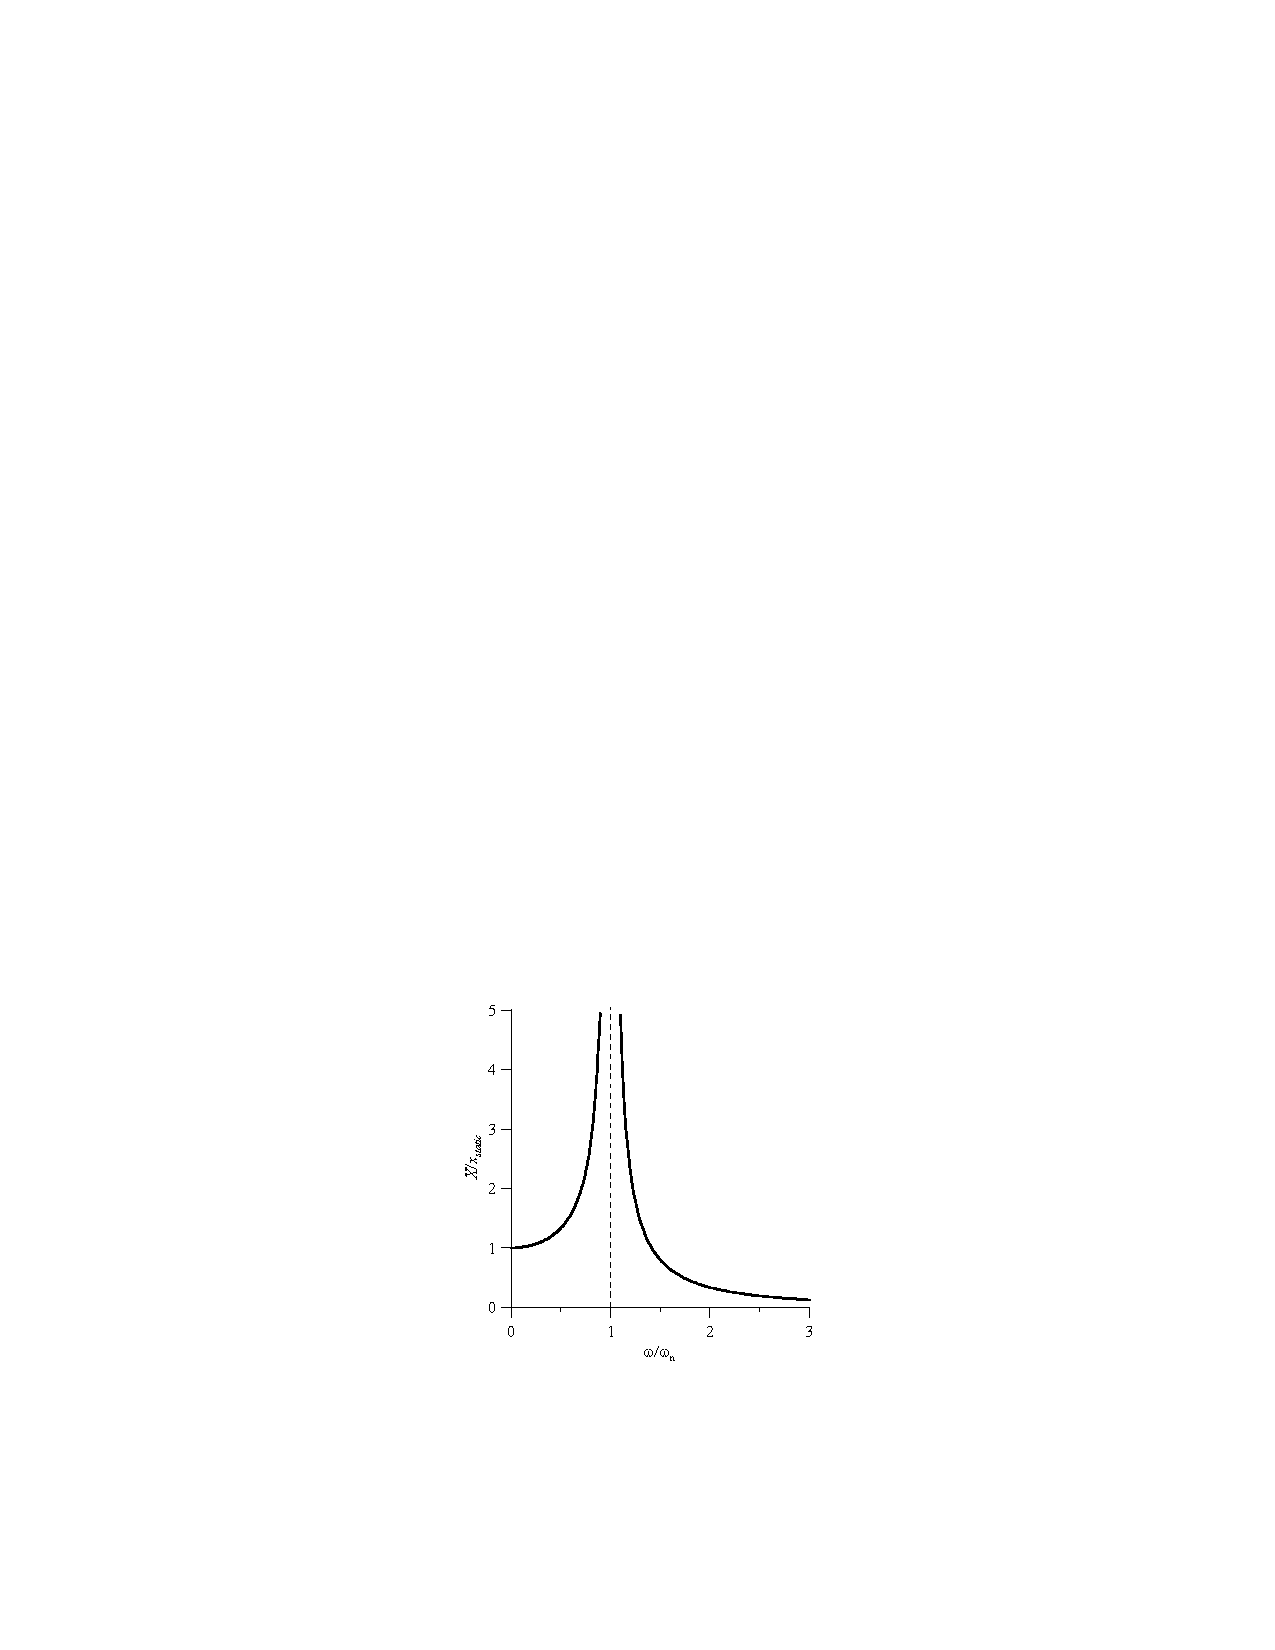
\includegraphics[width=0.6\textwidth]{amplitudefrequencycharacteristic.pdf}
	\caption{Amplitude-frequency characteristic. Extracted from \cite[2.2.2]{dynamicslecturenote}}
	\label{fig:amplitude-frequency-characteristic}
\end{figure}


\section{Introduction to the dynamics of railway bridges}

\cite{fryba1996dynamics}Dynamics of railway bridges is concerned with the study of deflections and stresses in railway bridges. The loads are represented by the moving wheel and axle forces, by means of which railway vehicles transmit their load and inertia actions to railway bridges. A survey of the dynamic effects of vehicles on railway bridges is given in Figure.\ref{fig:dynamic effects}

\begin{figure}[h]
	\centering
	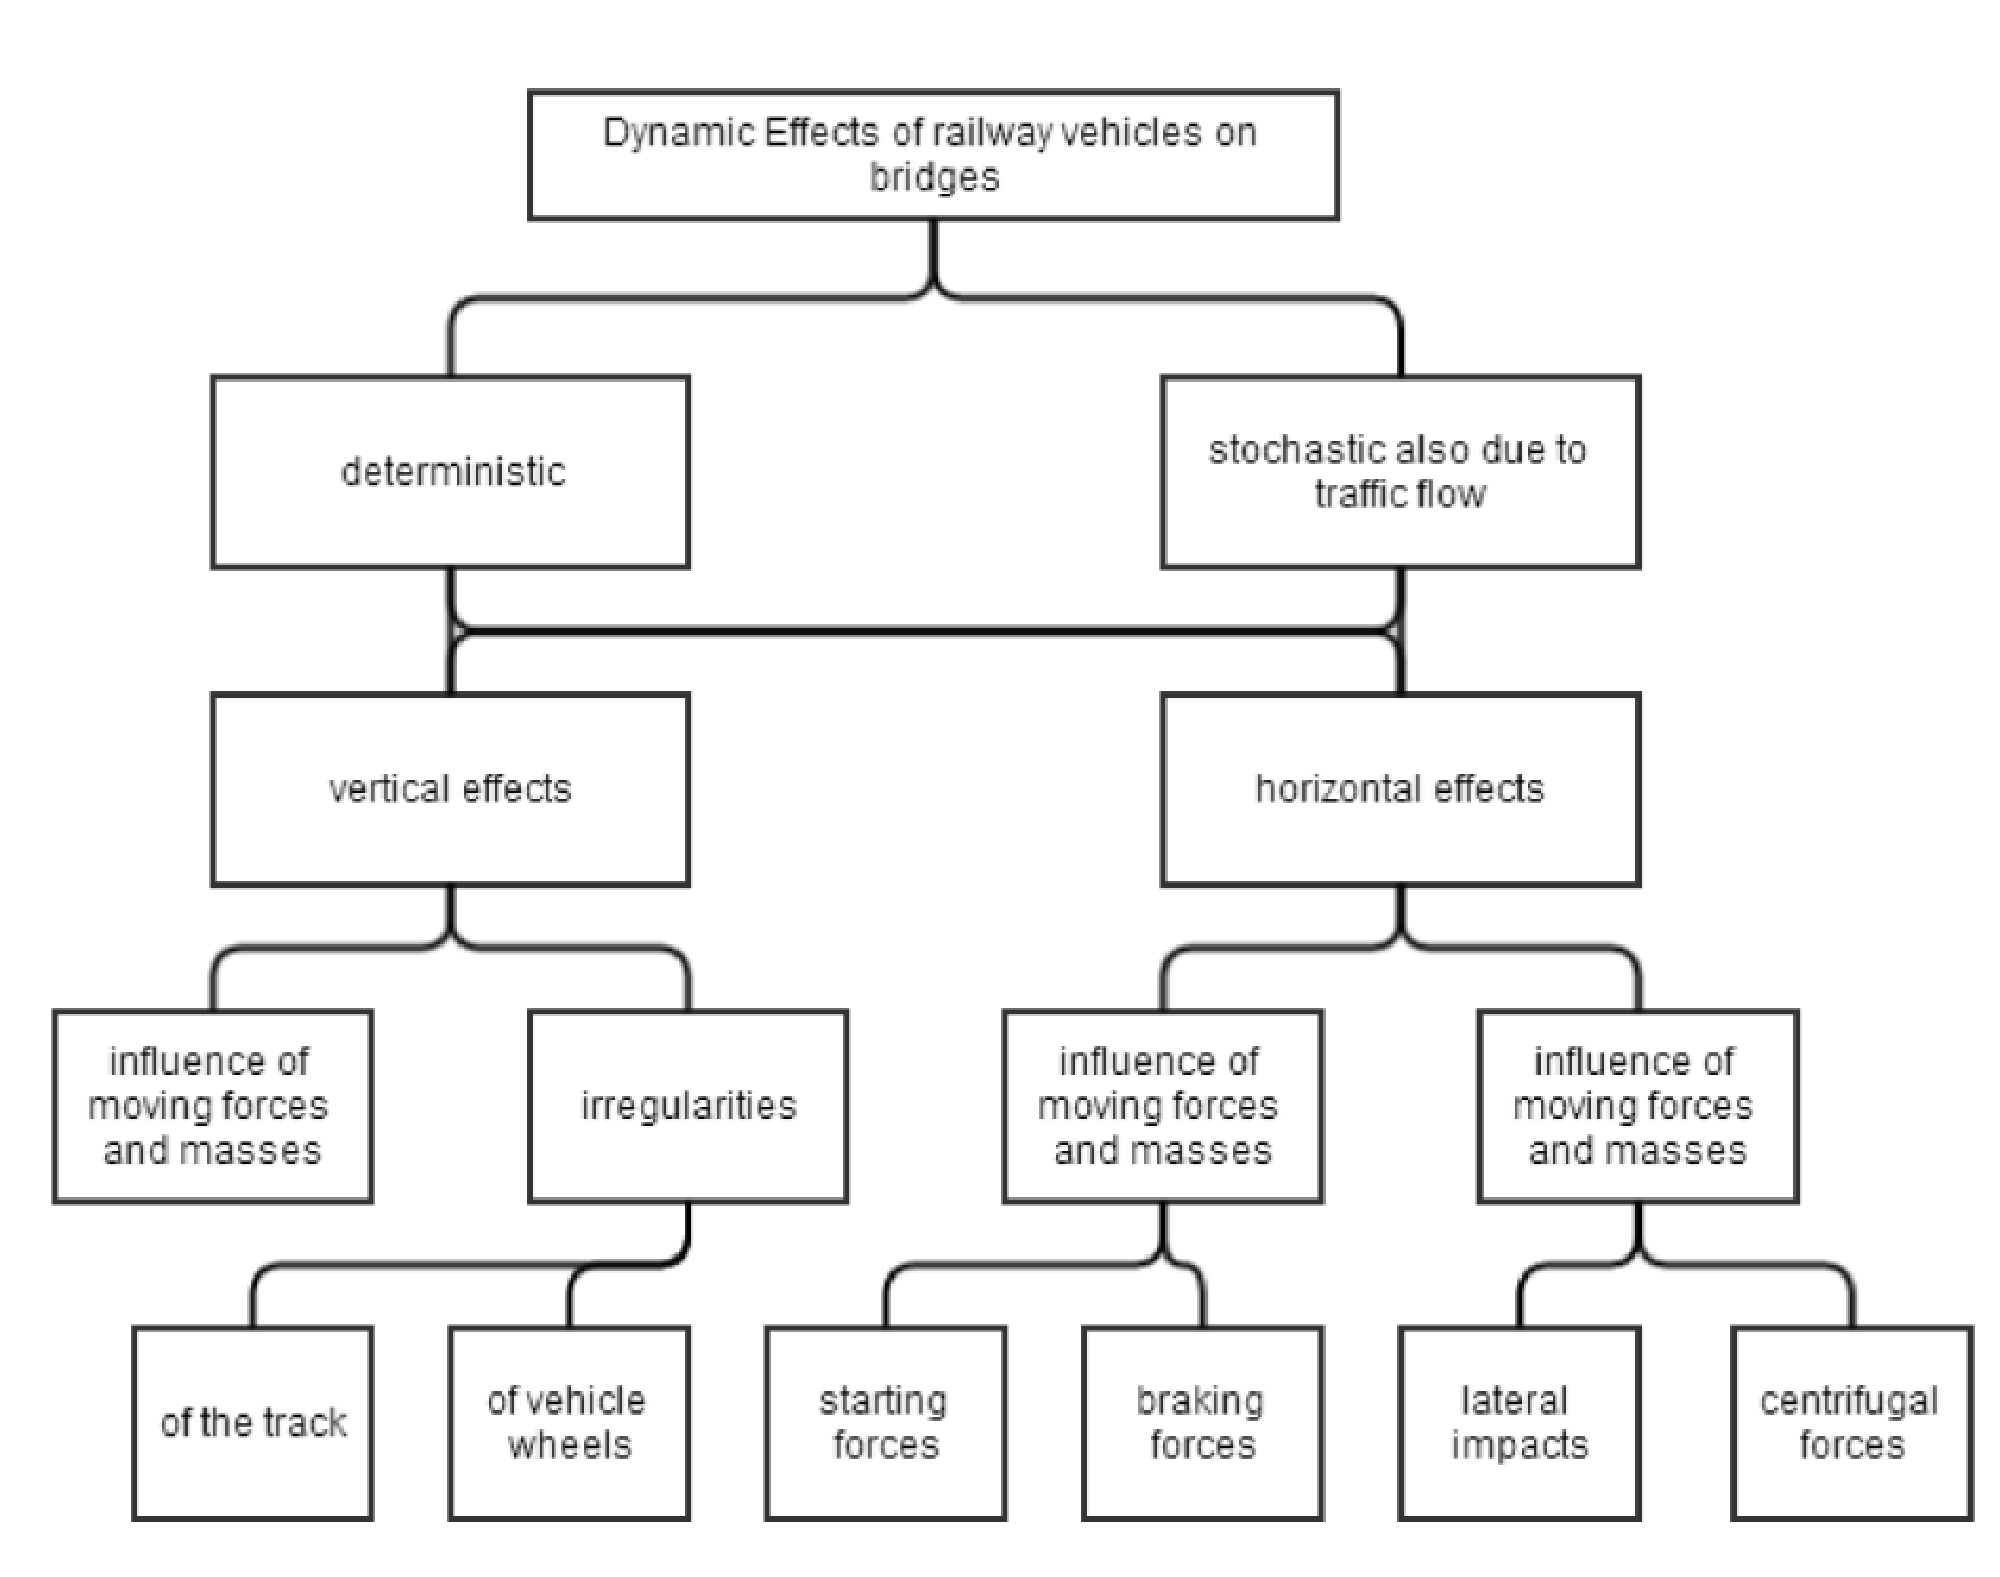
\includegraphics[width=0.6\textwidth]{dynamiceffects.pdf}
	\caption{Dynamic effects of railway vehicles on bridges. Extracted from \cite[1.1]{fryba1996dynamics} }
	\label{fig:dynamic effects}
\end{figure}

\subsection{Factors influencing dynamic behaviour}
As stated in\cite[6.4.2]{EC12} there are 11 factors influencing dynamic behaviour of a railway bridge. The principal factors which influence dynamic behaviour are:
\begin{enumerate}[-]
	\item the speed of traffic across the bridge
	\item the span L of the element and the influence line length for deflection of the element being considered
	\item the mass of the structure
	\item the natural frequencies of the whole structure and relevant elements of the structure and the associated mode shapes (eigenforms) along the line of the track
	\item the number of axles, axle loads and the spacing of axles
	\item the damping of the structure
	\item vertical irregularities in the track
	\item the unsprung/sprung mass and suspension characteristics of the vehicle
	\item the presence of regularly spaced supports of the deck slab and/or track (cross girders, sleepers etc.)
	\item vehicle imperfections (wheel flats, out of round wheels, suspension defects etc.)
	\item the dynamic characteristics of the track (ballast, sleepers, track components etc.)
\end{enumerate}

Other factors may include:

\begin{enumerate}

	\item The track number of the bridge and their alignment. 
	\item Multiple trains running on bridge simultaneously. 
	\item Track alignment

\end{enumerate}



\section{Vertical Dynamic effects}
As stated in EN 1991-2\cite{EC12}, the static stress and deformations (and associated bridge deck acceleration) induced in a bridge are increased and decreased under the effects of moving traffic by the following:

\begin{enumerate}[-]
	\item the rapid rate of loading due to the speed of traffic crossing the structure and the inertial response (impact) of the structure,
	\item the passage of successive loads with approximately uniform spacing which can excite the structure and under certain circumstances create resonance (where the frequency excitation(or a multiple there of) matches a natural frequency of the structure (or a multiple there of), there is a possibility that the vibrations caused by successive axles running onto the structure will be excessive),
	\item variations in wheel loads resulting from track or vehicle imperfections (including wheel irregulations).
\end{enumerate}
For determining the effects (stresses, deflections, bridge deck acceleration etc.) of rail traffic actions the above effects shall be taken into account.


\subsection{Train Actions}
See section \ref{designprocedures}


\subsection{Wind Actions}
The nature of the wind load is dynamic. This means that its magnitude varies with respect to time and space.

According to \cite{mohammadi2013wind}: The limitations behind the applications of the EN-1991-1-4, Eurocode1, actions on structures-general actions-wind load-part 1-4, lead the structural designers to a great confusion. This may be due to the fact that, EC1 provides only the guid- ance for the bridges whose fundamental mode of vibrations have constant sign (e.g. simply supported structures) or a simple linear sign (e.g. cantilever structures) and these modes are the governing mode of vibrations of the structure; it analyzes only the along-wind response of the structure and not the cross wind response and the simplified methods recommended in this code are covering only the structures with simple geometrical configurations.

\section{Horizontal transverse dynamic effects}
There's only one criterion in the Eurocodes mentioned that the bridge's first lateral natural frequency should no lower that 1.2 Hz. Dynamic analyses are required if this criterion is not met. 

However, as more and more long-span bridges are built nowadays, this requirement is not valid for more bridges. This is because, in general, the lateral natural frequency of a bridge decreases when span increases. For bridges with span longer than 100m, there's few bridge can have a lateral frequency higher than 1.2Hz, according to senior engineers' designing experience.

So it is vital to discuss horizontal dynamic effects for the sake of longer span bridges. In additional, study the requirements for horizontal vibration of railway bridges to make the results of dynamic analysis usable.

\subsection{Sources induce transverse dynamic reactions}
According to \cite{da2007dynamic}\cite{fryba1996dynamics}\cite{EC12}, following sources are identified:

\begin{enumerate} [-]
	\item Horizontal track irregularities
	\item Sinusoidal motion of conical wheels along cylindrical rail heads
	\item Centrifugal forces on curved tracks
	\item Train switches
\end{enumerate}

\subsection{Horizontal vibration of a beam}

Fryba\cite{fryba1996dynamics} described the first two sources in mathematical terms:
Consider a simply supported beam loaded by moving train loading, horizontal vibrations of the beam in a transverse direction $ w(x,t) $ are generated by lateral random forces $ H_n (t) $ due to random irregularities and sinusoidal motion. The differential equation for the deformation is:

\begin{equation}
	EI_yw^{IV}(w,t)+\mu \ddot{w} (x,t)=\sum_{n=1}^{N} \varepsilon_n\delta(x+d_n-ct)H_n(t) 
\end{equation}

where $ H_n(t) $ stands for forces due to random irregularities and sinusoidal motion. $ H_n(t) $ is of a typically random character and can be replaced by horizontal transverse forces with zero mean values. See Figure.~\ref{fig:trackirrg} for example.

\cite[Table 9.1]{fryba1996dynamics} gives sample of natural frequencies of steel truss bridges with open deck. Shown as follow Table~\ref{tab:spatialvibrationsteel}. Please note that truss bridges have high stiffness.

\begin{table}[h]
	\centering
	\begin{tabular}{ccccc}
		\hline
		\multirow{2}{*}{Vibration Type} & \multirow{2}{*}{Symbol} & \multirow{2}{*}{j} & \multicolumn{2}{c}{Bridge with span} \\
		\cline{4-5}
		 & & & $ l=25.85m $ & $ l=48.4m $\\
		\hline
		\multirow{3}{*}{Vertical} & \multirow{3}{*}{$ f_j $} & 1 & 8.7 & 5.4\\
		 & & 2 & 34.7 & 21.5 \\
	 	 & & 3 & 78.1 & 48.3 \\
	 	\hline
	 	\multirow{9}{*}{Horizontal} & \multirow{3}{*}{$ f_{hj} $} & 1 & 15.3 & 4.7 \\
	 	 & & 2 & 61.1 & 19.0 \\
	 	 & & 3 & 137.5 & 42.7 \\
	 	\cline{2-5}
	 	 & \multirow{3}{*}{$ f_{yj} $} & 1 & 14.8 & 4.7 \\
	 	 & & 2 & 53.9 & 18.1 \\
	 	 & & 3 & 107.4 & 38.8 \\ 
	 	\cline{2-5}
	 	 & \multirow{3}{*}{$ {f}'_{yj} $} & 1 & 14.7 & 4.6 \\
	 	 & & 2 & 52.5 & 17.5 \\
	 	 & & 3 & 101.7 & 36.4 \\ 
	 	\cline{2-5}
	 	\hline
	 	\multirow{9}{*}{Torsional} & \multirow{3}{*}{$ f_{\xi j} $} & 1 & 35.7 & 19.2 \\
	 	 & & 2 & 71.3 & 38.4 \\
	 	 & & 3 & 107.0 & 57.7 \\
	 	\cline{2-5}
	 	 & \multirow{3}{*}{$ f_{\varphi j} $} & 1 & 34.9 & 16.7 \\
	 	 & & 2 & 73.5 & 35.4 \\
	 	 & & 3 & 117.4 & 56.9 \\ 
	 	\cline{2-5}
	 	 & \multirow{3}{*}{$ {f}'_{\varphi j} $} & 1 & 36.5 & 19.7 \\
	 	 & & 2 & 77.6 & 41.9 \\
	 	 & & 3 & 126.4 & 67.5 \\ 
	 	\hline
	\end{tabular}
	\caption{Spatial vibrations of steel truss bridges with open bridge deck}
	\label{tab:spatialvibrationsteel}
\end{table}


\begin{figure}[p]
	\centering
	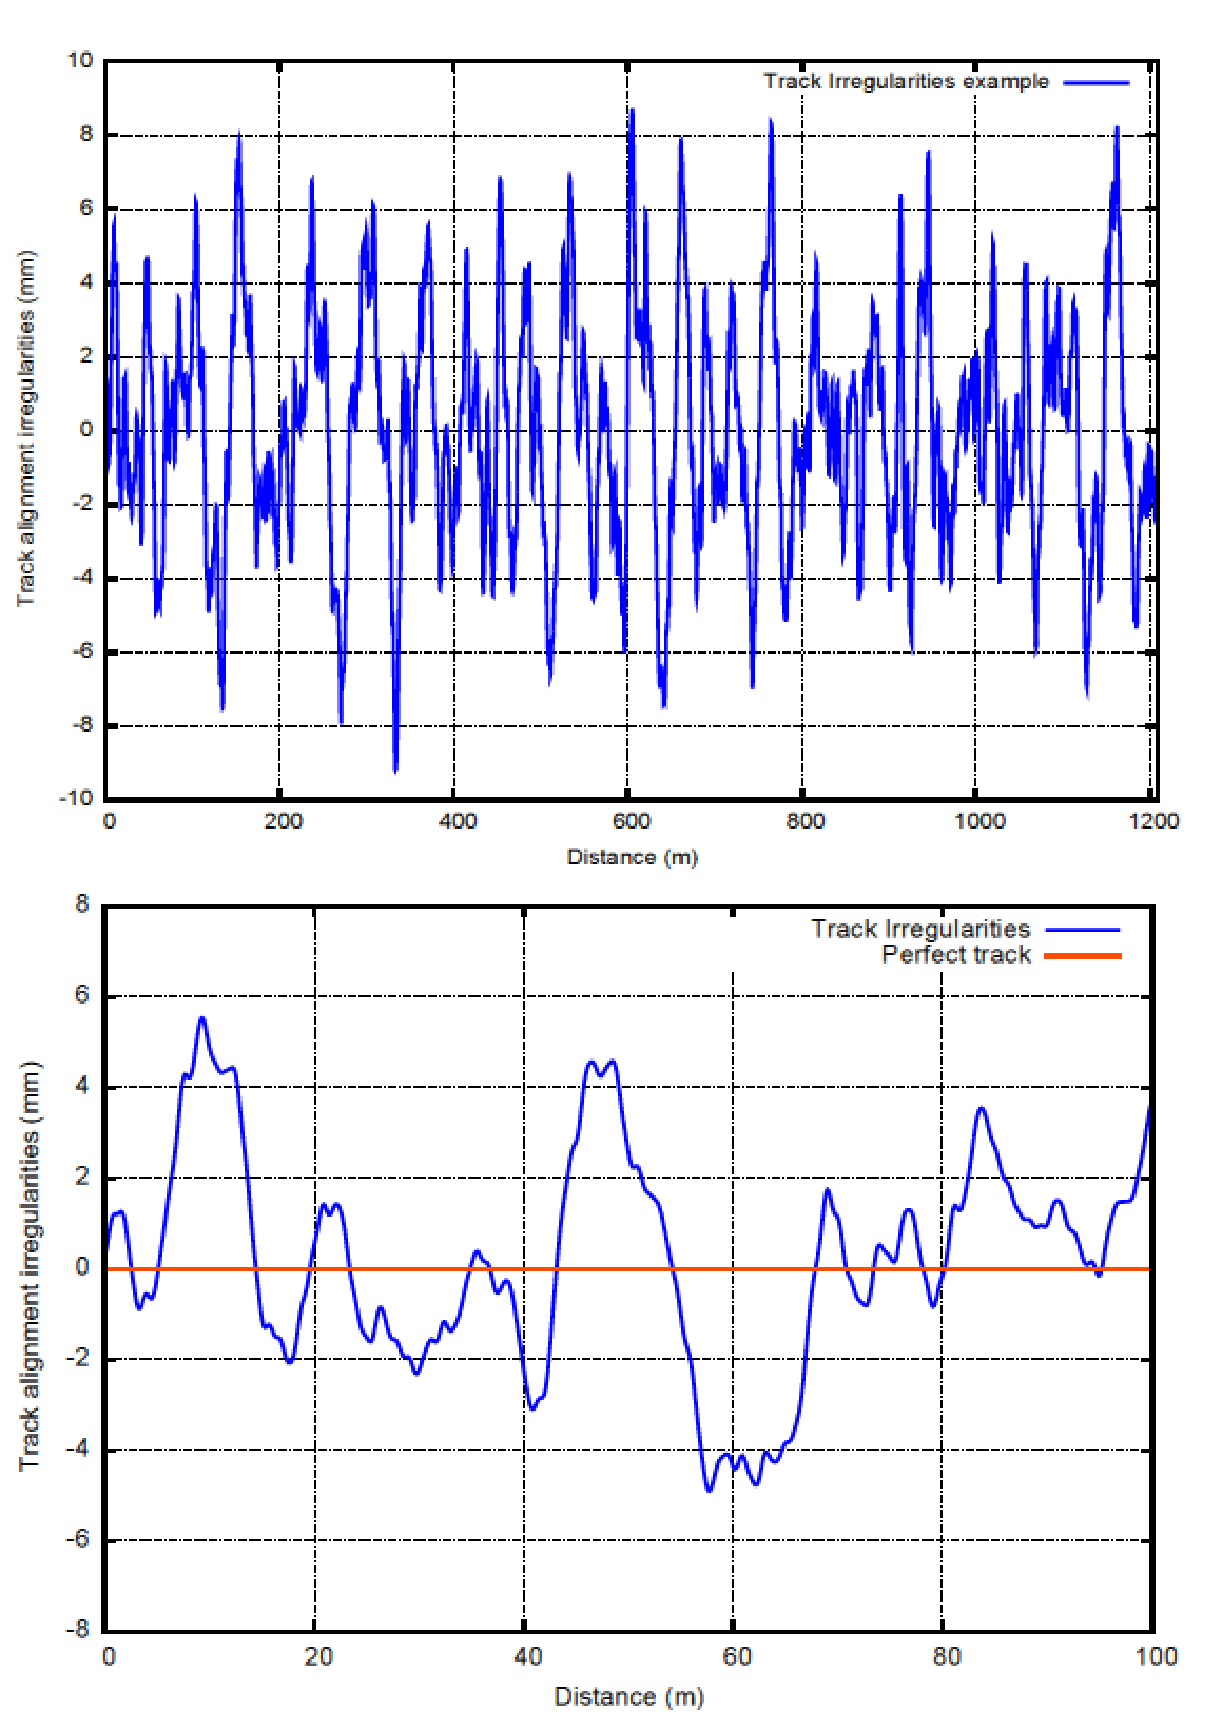
\includegraphics[width=0.8\textwidth]{trackirregularities.pdf}
	\caption{Example of a track lateral alignment irregularities profile for a track with low irregularities in a total length of 1209m.  Extracted from \cite{da2007dynamic}}
	\label{fig:trackirrg}
\end{figure}


\subsubsection{Centrifugal forces}
In \cite[6.5.1]{EC12} specifies following principles about centrifugal forces act on railway bridges:

Where the track on a bridge is curved over the whole or part of the length of the bridge, the centrifugal force and the track cant shall be taken into account.

The centrifugal forces should be taken to act outwards in a horizontal direction at a height of 1.80m above the running surface (see \cite[Figure 1.1]{EC12}). For some traffic types, e.g. double stacked containers, an increased value of $h_t$ should be specified.

The centrifugal force shall always be combined with the vertical load. The centrifugal force shall not be multiplied by the dynamic factor $\varPhi_1$ or $\varPhi_3$.

The characteristic value of the centrifugal force shall be determined according to the following equations:

\begin{equation}
	Q_tk=\frac{v^2}{g \cdot r}(f \cdot Q_{vk})=\frac{V^2}{127r}(f \cdot Q_{vk})
\end{equation}

\begin{equation}
	q_{tk}=\frac{v^2}{g \cdot r}(f \cdot q_{vk})=\frac{V^2}{127r}(f \cdot q_{vk})
\end{equation}

where:

\begin{tabular}{ll}
$Q_{tk}$,$q_{tk}$ & Characteristic values of the centrifugal forces\\
$Q_{vk}$,$q_{vk}$ & Characteristic values of the vertical loads specified in \cite[6.3]{EC12}\\
$f$ & Reduction factor, see below \\
$v$ & Maximum speed in accordance with \cite[6.5.1(5)]{EC12}[m/s]\\
$V$ & Maximum speed in accordance with \cite[6.5.1(5)]{EC12}[km/h]\\
$g$ & Acceleration due to gravity [9.81$m/s^2$]\\
$r$ & Radius of curvature [m].
\end{tabular}

For Load Model 71 (and where required Load Model SW/0) the reduction factor $f$ is given by:

\begin{equation}
	f=[1-\frac{V-120}{1000}(\frac{814}{V}+1.75)(1-\sqrt{\frac{2.88}{L_f}})]
\end{equation}

\subsection{Requirements for traffic safety(horizontal)}
Requirements other than bridge first lateral frequency higher than 1.2Hz. Since there's no further requirements mentioned by Eurocode, following requirements are gathered from other European codes, eg. British standards, UIC leaflet, etc.

\begin{enumerate}[-]
	\item Requirements regarding traffic safety for vehicles
	\begin{enumerate}
		\item Guiding Force: \cite{code2005518} , \cite{en200714363} and\cite{cuadrado2008analysis} propose safty limitations against railway vehicle overturning. From\cite{en200714363} the maximum guiding force for a vehicle with a load per axle of 170kN(AVE) is 66kN per axle and 48kN per axle for a vehicle with a load per axle of 112kN(ICE2). For the R1 freight wagon(load per axle of 245kN), the maximum guiding force per axle is 78kN.
		\item Maximum lateral acceleration of the railway vehicle: proposed by \cite{13803}
	\end{enumerate}
	\item Requirements regarding safety for bridge\\
	\cite{EC0} A2.4.4.1(2): Horizontal transverse deflection(to ensure acceptable horizontal track radii) and horizontal rotation of a deck about a vertical axis at ends of a deck(to ensure acceptable acceptable horizontal track geometry and passenger comfort)
\end{enumerate}


\subsection{Requirements for traffic safety on derailment: Railway vehicle derailment mechanism and safety criteria}

Derailment mechanisms
\begin{enumerate}
	\item vehicle resonant response
	\item lateral instability
	\item vehicle overturning
	\item vertical wheel unloading
	\item flange climb
	\item rail roll-over
	\item track panel shift
	\item longitudinal train forces
\end{enumerate}

The four types of derailment: flange climb derailment, derailment caused by guage widening and rail roll-over, derailment caused by track panel shift, derailment cause by vehicle lateral instability have a common cause of high lateral force at the wheel-rail interface. According to \cite[Chapter 8, IV]{iwnicki2006handbook} any conditions that lead to high lateral forces or lead to lower the ability of the system to sustain the force should be corrected. 

\subsubsection{Flange climb derailment}
Wheel flange climb derailments are caused by wheels climbing onto the top of the railhead then further running over the rail. Wheel climb derailments generally occur in situations where the wheel experiences a high lateral force combined with circumstances where the vertical force is reduced on the flanging wheel. The high lateral force is usually induced by a large wheelset angle-of-attack. The vertical force on the flanging wheel can be reduced significantly on bogies having poor vertical wheel load equalisations, such as when negotiating rough track, large track twist, or when the car is experiencing roll resonances. 

\begin{figure}[h]
	\centering
	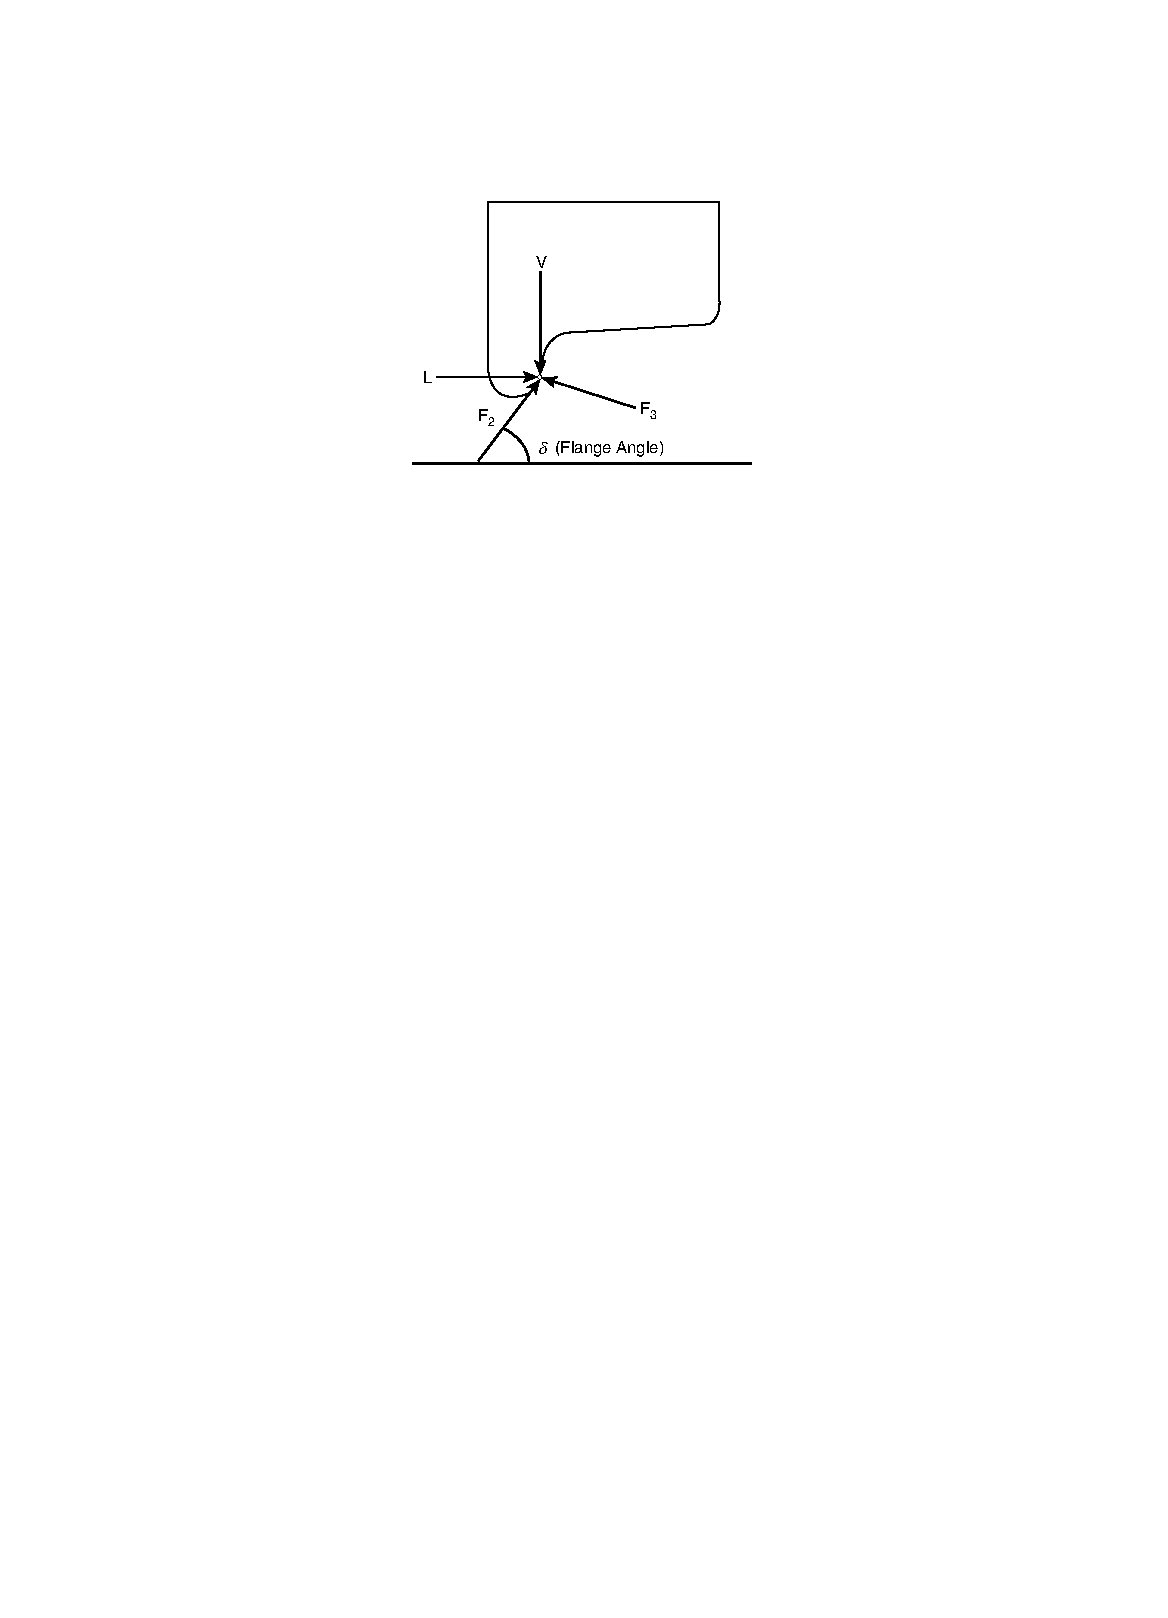
\includegraphics[width=0.4\textwidth]{forcesatflangecontactlocation.pdf}
	\caption{Forces at flange contact location. Extracted from \cite[Figure8.4]{iwnicki2006handbook}}
	\label{fig:forcesatflangecontactlocation}
\end{figure}

The criterion L/V ratio can be expressed as:

\begin{equation}
	\frac{L}{V}=\frac{\tan \delta -\frac{F_2}{F_3}}{1+\frac{F_2}{F_3}\tan \delta}
\end{equation}

Nadal's famous L/V ratio limiting criterion, given by Equation.\ref{eq:nadalcriterion}, was proposed for the saturated condition $F_2/F_3=\mu$

\begin{equation}\label{eq:nadalcriterion}
	\frac{L}{V}=\frac{\tan \delta - \mu}{1+ \mu \tan \delta}
\end{equation}

\subsubsection{Derailment caused by guage widening and rail rollover}
Derailments caused by guage widening usually involve a combination of wide gauges and large lateral rail defections(rail roll), as shown in Figure\ref{fig:gaugewideningderailment}. Large lateral forces from the wheels act to spread the rails in curves. Both rails may experience significant lateral translation and/or railhead roll, which often cause the nonflanging wheel to drop between rails.

\begin{figure}[h]
	\centering
	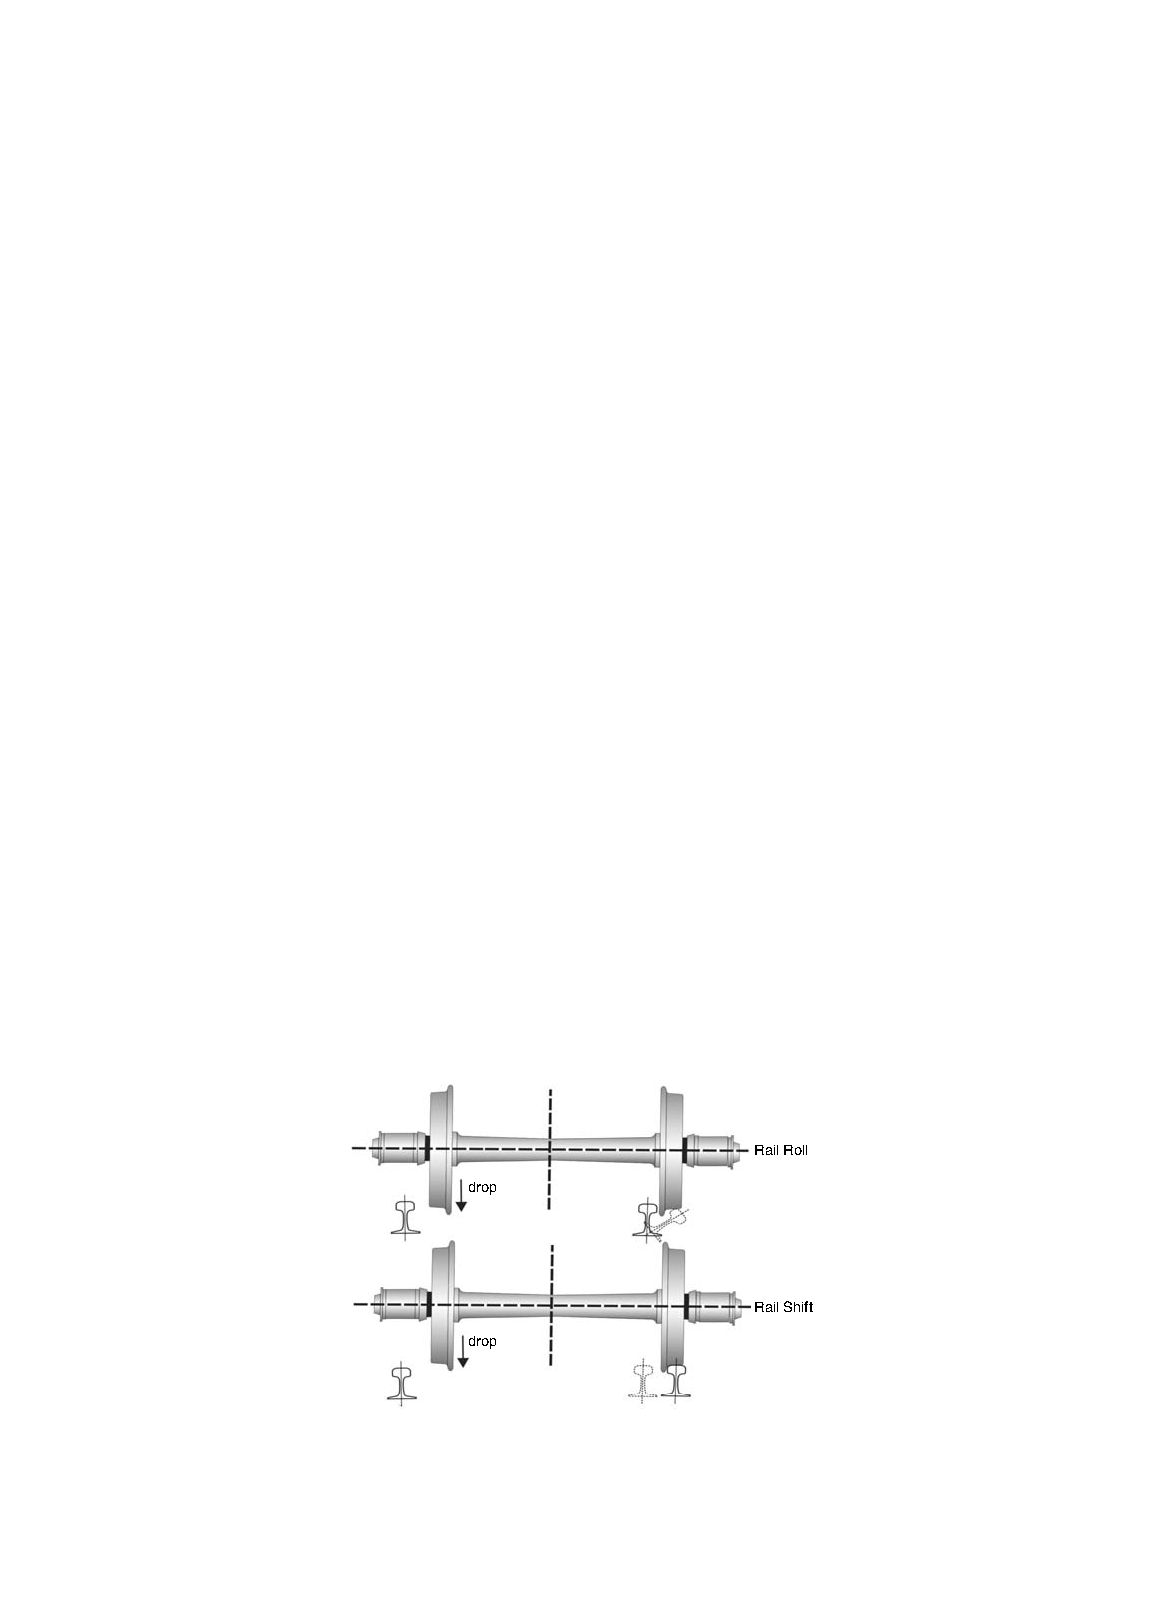
\includegraphics[width=0.8\textwidth]{gaugewideningderailment.pdf}
	\caption{Gauge widening derailment. Extracted from \cite[Figure8.18]{iwnicki2006handbook}}
	\label{fig:gaugewideningderailment}
\end{figure}

\paragraph{AAR Chapter XI rail roll criterion}
The AAR Chapter XI rail roll criterion is established by using the L/V ratio. The roll moment about the pivot point is given by,

\begin{equation}
	M=Vd-Lh
\end{equation}

under an equilibrium condition, just before the rail starts to roll, $M$ approaches to zero, then,

\begin{equation}
	\frac{L}{V}=\frac{d}{h}
\end{equation}

This L/V ratio is considered as the critical value to evaluate the risk of rail roll. When the L/V ratio is larger than the ratio of $d/h$, the risk of rail roll becomes high. The critical L/V ratio for rail roll can vary from above 0.6 for contact at the gauge side to approximately 0.2 when the contact position is at the far-field side based on the dimension of the rails. This is because the distance $d$ is reduced. Note that this L/V ratio is calculate assuming that neither the rail fasteners nor the torsional stiffness of the rail section provide any restraint.

\subsubsection{Derailment caused by track panel shift}
Track panel shift is the cumulative lateral displacement of the track panel, including rails, tie plates and ties, over the ballast, as shown in Figure\ref{fig:lateraltrackpanelshift}. A small shift of these components may not immediately cause the loss of guidance to bogies. However, as the situation gradually depreciates to a certain level, wheels could lose guidance and drop to the ground at some speed. The derailments caused by track panel usually result in one wheel falling between the rails and the other falling outside of the track.

\begin{figure}[h]
	\centering
	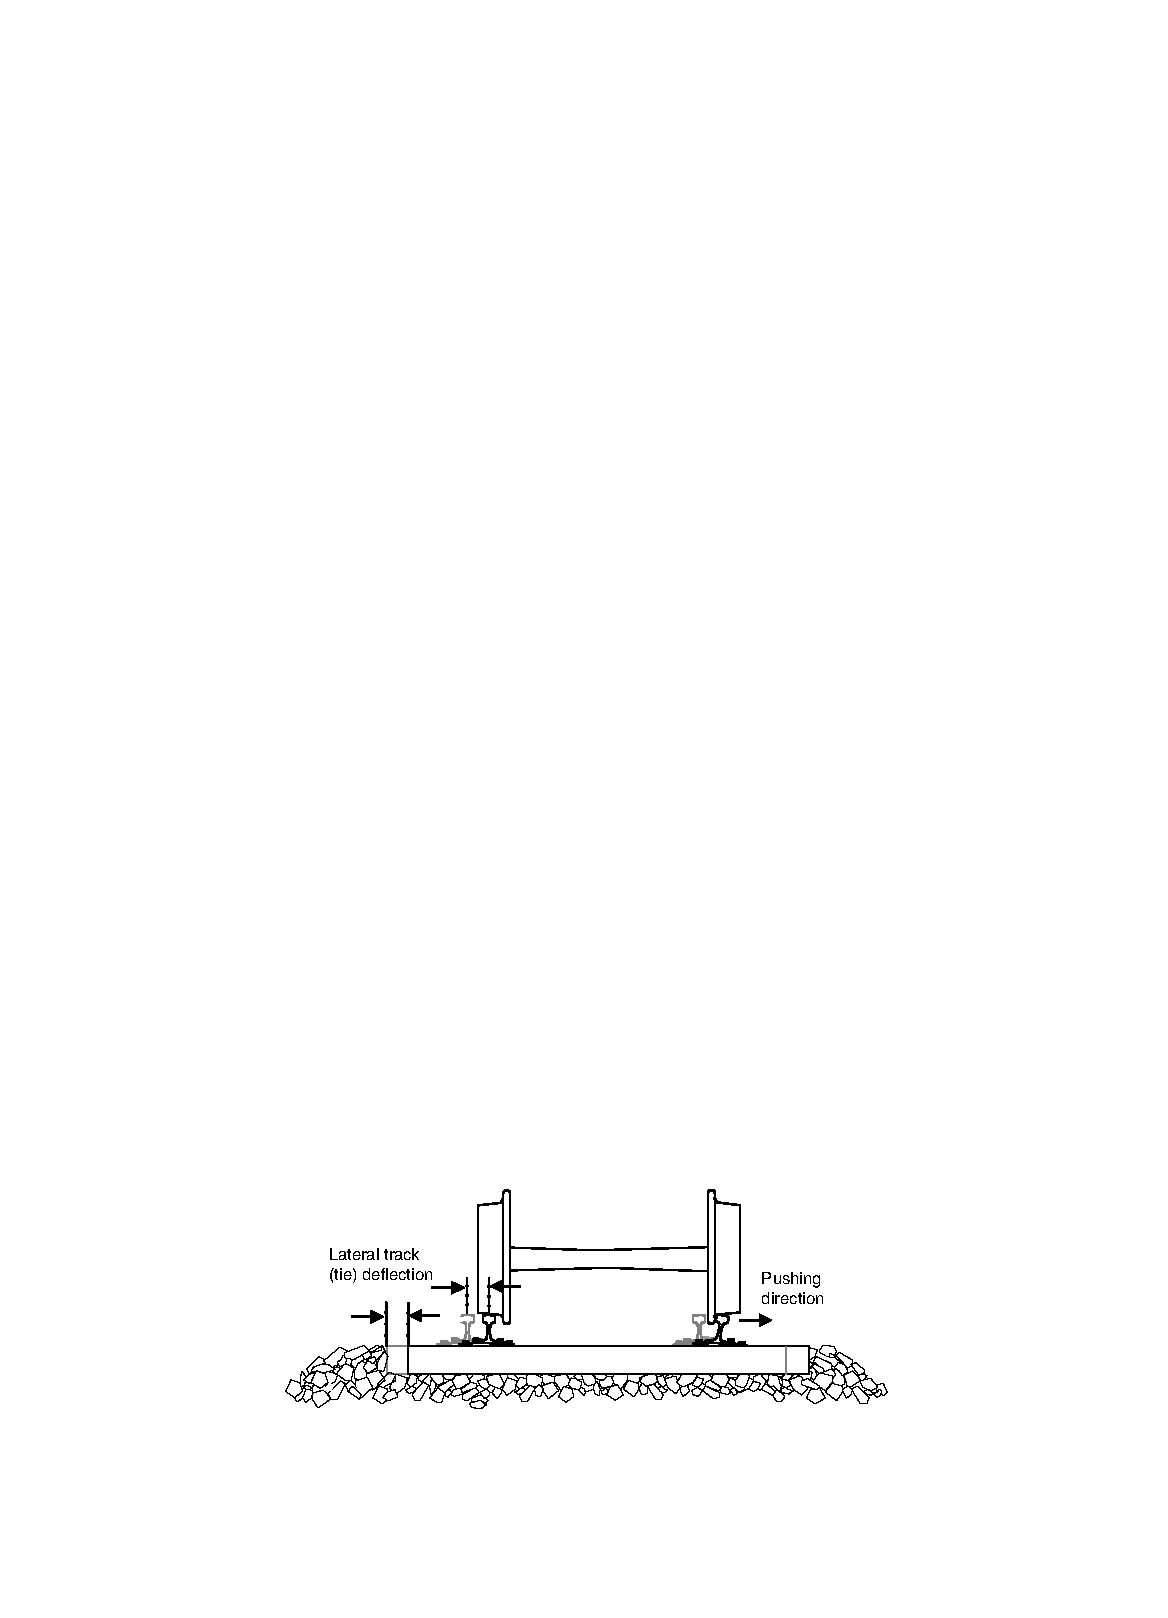
\includegraphics[width=0.8\textwidth]{lateraltrackpanelshift.pdf}
	\caption{Lateral track panel shift. Extracted from \cite[Figure8.27]{iwnicki2006handbook}}
	\label{fig:lateraltrackpanelshift}
\end{figure}

\paragraph{Panel shift criterion}
Researched by the French National Railways suggested that the limiting lateral axle load can be defined in a general expression for preventing excessive track panel shift:

\begin{equation}
	L_c = aV+b
\end{equation}

where $L_c$ is the critical lateral load and $V$ is the vertical axle load. \cite[Table 8.2]{iwnicki2006handbook} lists two groups of suggested valued of $a$ and $b$. It is possible that different values for $a$ and $b$ can be specified in different area.

\subsubsection{Derailment caused by vehicle lateral instability}
On tangent track, the wheelset generally oscillates around the track centre due to any vehicle and track irregularities, as shown in Figure\ref{fig:wheelsetoscillatesaroundthetrackcentre}. This movement occurs because vehicle and track are never absolutely smooth and symmetric. This self-centring capability of a wheelset is induced by the coned shape of the wheel tread. However, as speed is increased, if the whelset conicity is high, the lateral movement of wheelset, as well as the associated bogie and car body motion, can cause oscillations with large amplitude  and a well-defined wavelength. The lateral movements are limited only by the contact of the wheel flanges with the rail. This vehicle dynamic response is also termed as vehicle hunting, and can produce high lateral forces to damage track to cause derailments.

\begin{figure}[h]
	\centering
	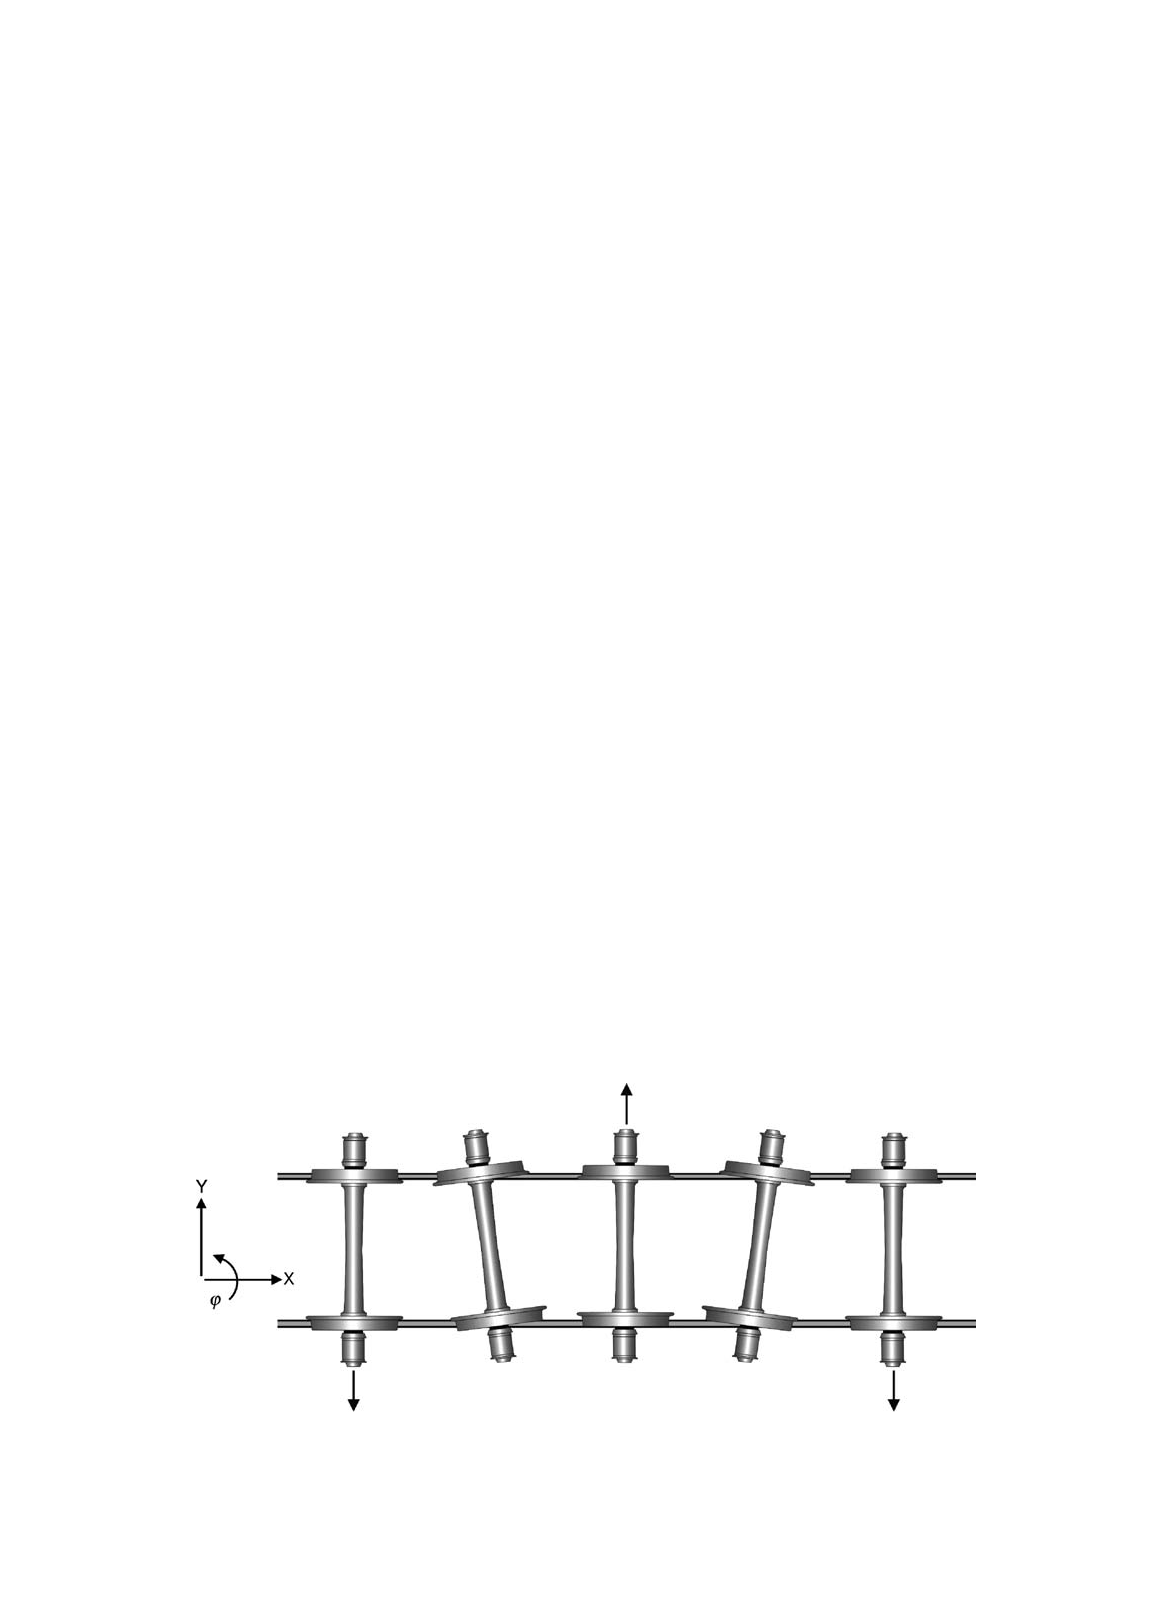
\includegraphics[width=0.8\textwidth]{wheelsetoscillatesaroundthetrackcentre.pdf}
	\caption{Wheelset oscillates around the track centre. Extracted from \cite[Figure8.28]{iwnicki2006handbook}}
	\label{fig:wheelsetoscillatesaroundthetrackcentre}
\end{figure}

Derailment cause by vehicle hunting can have derailment mechanisms of all four types discussed in the previous sections. The high lateral force induced from hunting may cause wheel flange climbing on the rail, gauge widening, rail roll-over, track panel shift, or combinations of these. The safety concerns for this type of derailment, usually occurring at higher speeds, make it an important area of study.

Hunting predominantly occurs in empty or lightweight vehicles. The critical hunting speed is highly dependent on the vehicle/track characteristics. Investigation of the critical speed for such a system with nonlinearities is to examine the vehicle response to a disturbance using a numerical solution of the equations of motion.

\subsection{Requirements for traffic serviceability(horizontal)}

The criteria Comfort Indexes for assessing ride comfort in railway vehicles proposed in \cite{12299}. This standard describes a methodology for assessing ride comfort as a function of longitudinal, vertical and transverse accelerations.

Comfort Index indicates the percentage of passengers experimenting discomfort in a specific situation. These indexes can be computed via empiric formula given in the standard, which depend on variables such as lateral acceleration, rate of change of acceleration and rolling velocity. All these values are filtered with a moving average filter that eliminates small wavelength components. Using this methodology for the computed worst-case situations, the comfort indexes have been found excellent, therefore no passenger should feel uncomfortable. 

\section{Torsional vibration}
According to \cite[9.1.3]{fryba1996dynamics}, the horizontal lateral forces of railway vehicles act on the rial top level,i.e. outside the cross section centroid of the bridge in the majority of cases. Let the difference of elevations be $ h $. Consequently, they affect the bridge by twisting moments $ hH_n(t) $. The differential equation of a beam due to simple torsion is 
\begin{equation}
	-GI_\xi \xi''(x,t)+\mu \ddot{\xi}(x,t)=\sum_{n=1}^{N}\varepsilon_n \delta (x+d_n-ct)h H_n(t)
\end{equation}

where $ \xi (x,t) $ is the rotation about the longitudinal beam axis x, $ G $ is the modulus of elasticity in shear, $ GI_\xi $ is the moment of torsional rigidity per unit length, $ \mu_\xi $ is the mass polar moment of inertia with regard to axis $ x $ per unit length.

\section{Theoretical bridge models}
According to \cite[Chapter.2]{fryba1996dynamics}, theoretical models of railway bridges are of two types

\begin{enumerate}[-]
	\item with continuously distributed mass
	\item with mass concentrated in material points(lumped mass)
	\item their combinations
\end{enumerate}

\subsection{Mass beams}
The most common simplified model for bridge is a simply supported Euler-Bernoulli beam model(see Figure.\ref{fig:massbeammodel}). The equation of motion of the beam expresses the equilibrium of forces per unit length:

\begin{figure}[h]
	\centering
	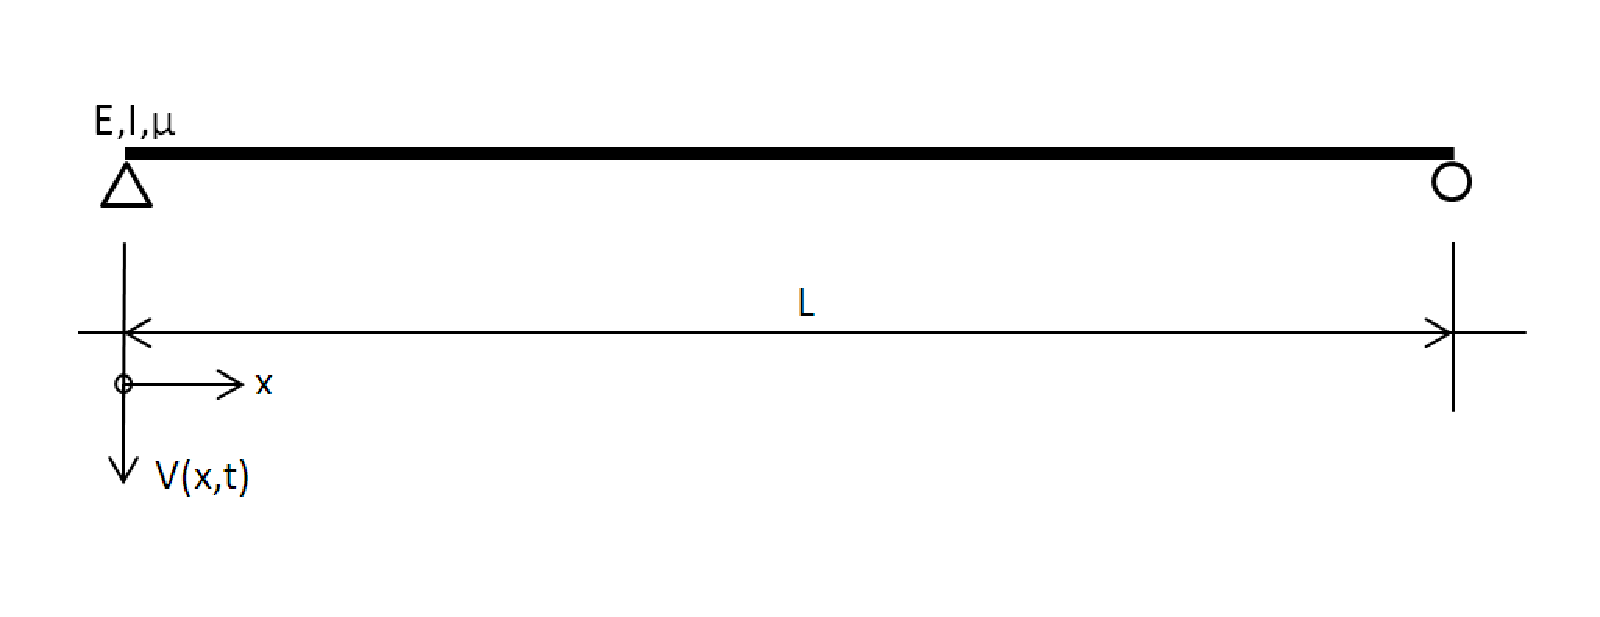
\includegraphics[width=0.8\textwidth]{massbeammodel.pdf}
	\caption{Mass beam model of span L}
	\label{fig:massbeammodel}
\end{figure}

\begin{equation}
	EI\dfrac{\partial^4v(x,t)}{\partial x^4}+\mu \dfrac{\partial^2 v(x,t)}{\partial t^2} + 2\mu \omega_b \dfrac{\partial v(x,t)}{\partial t} = f(x,t)
	\label{eq:massbeammodel}
\end{equation}

where:
\begin{enumerate}[]
	\item $ v(x,t) $:vertical deflection of the beam at the point $ x $ and at time $ t $
	\item $ E $:modulus of elasticity of the beam
	\item $ I $:moment of inertia of beam cross section
	\item $ \mu $:mass per unit length of the beam
	\item $ \omega_b $:circular frequency of viscous damping
	\item $ f(x,t) $:load at point $ x $ and time $ t $ per unit length of the beam
\end{enumerate}

\subsection{Continuous beam}
The continuous beam model is suitable for multi-span bridges in general. The equation of motion is the same as simple beam model in Equation\ref{eq:massbeammodel}. 

\begin{figure}[h]
	\centering
	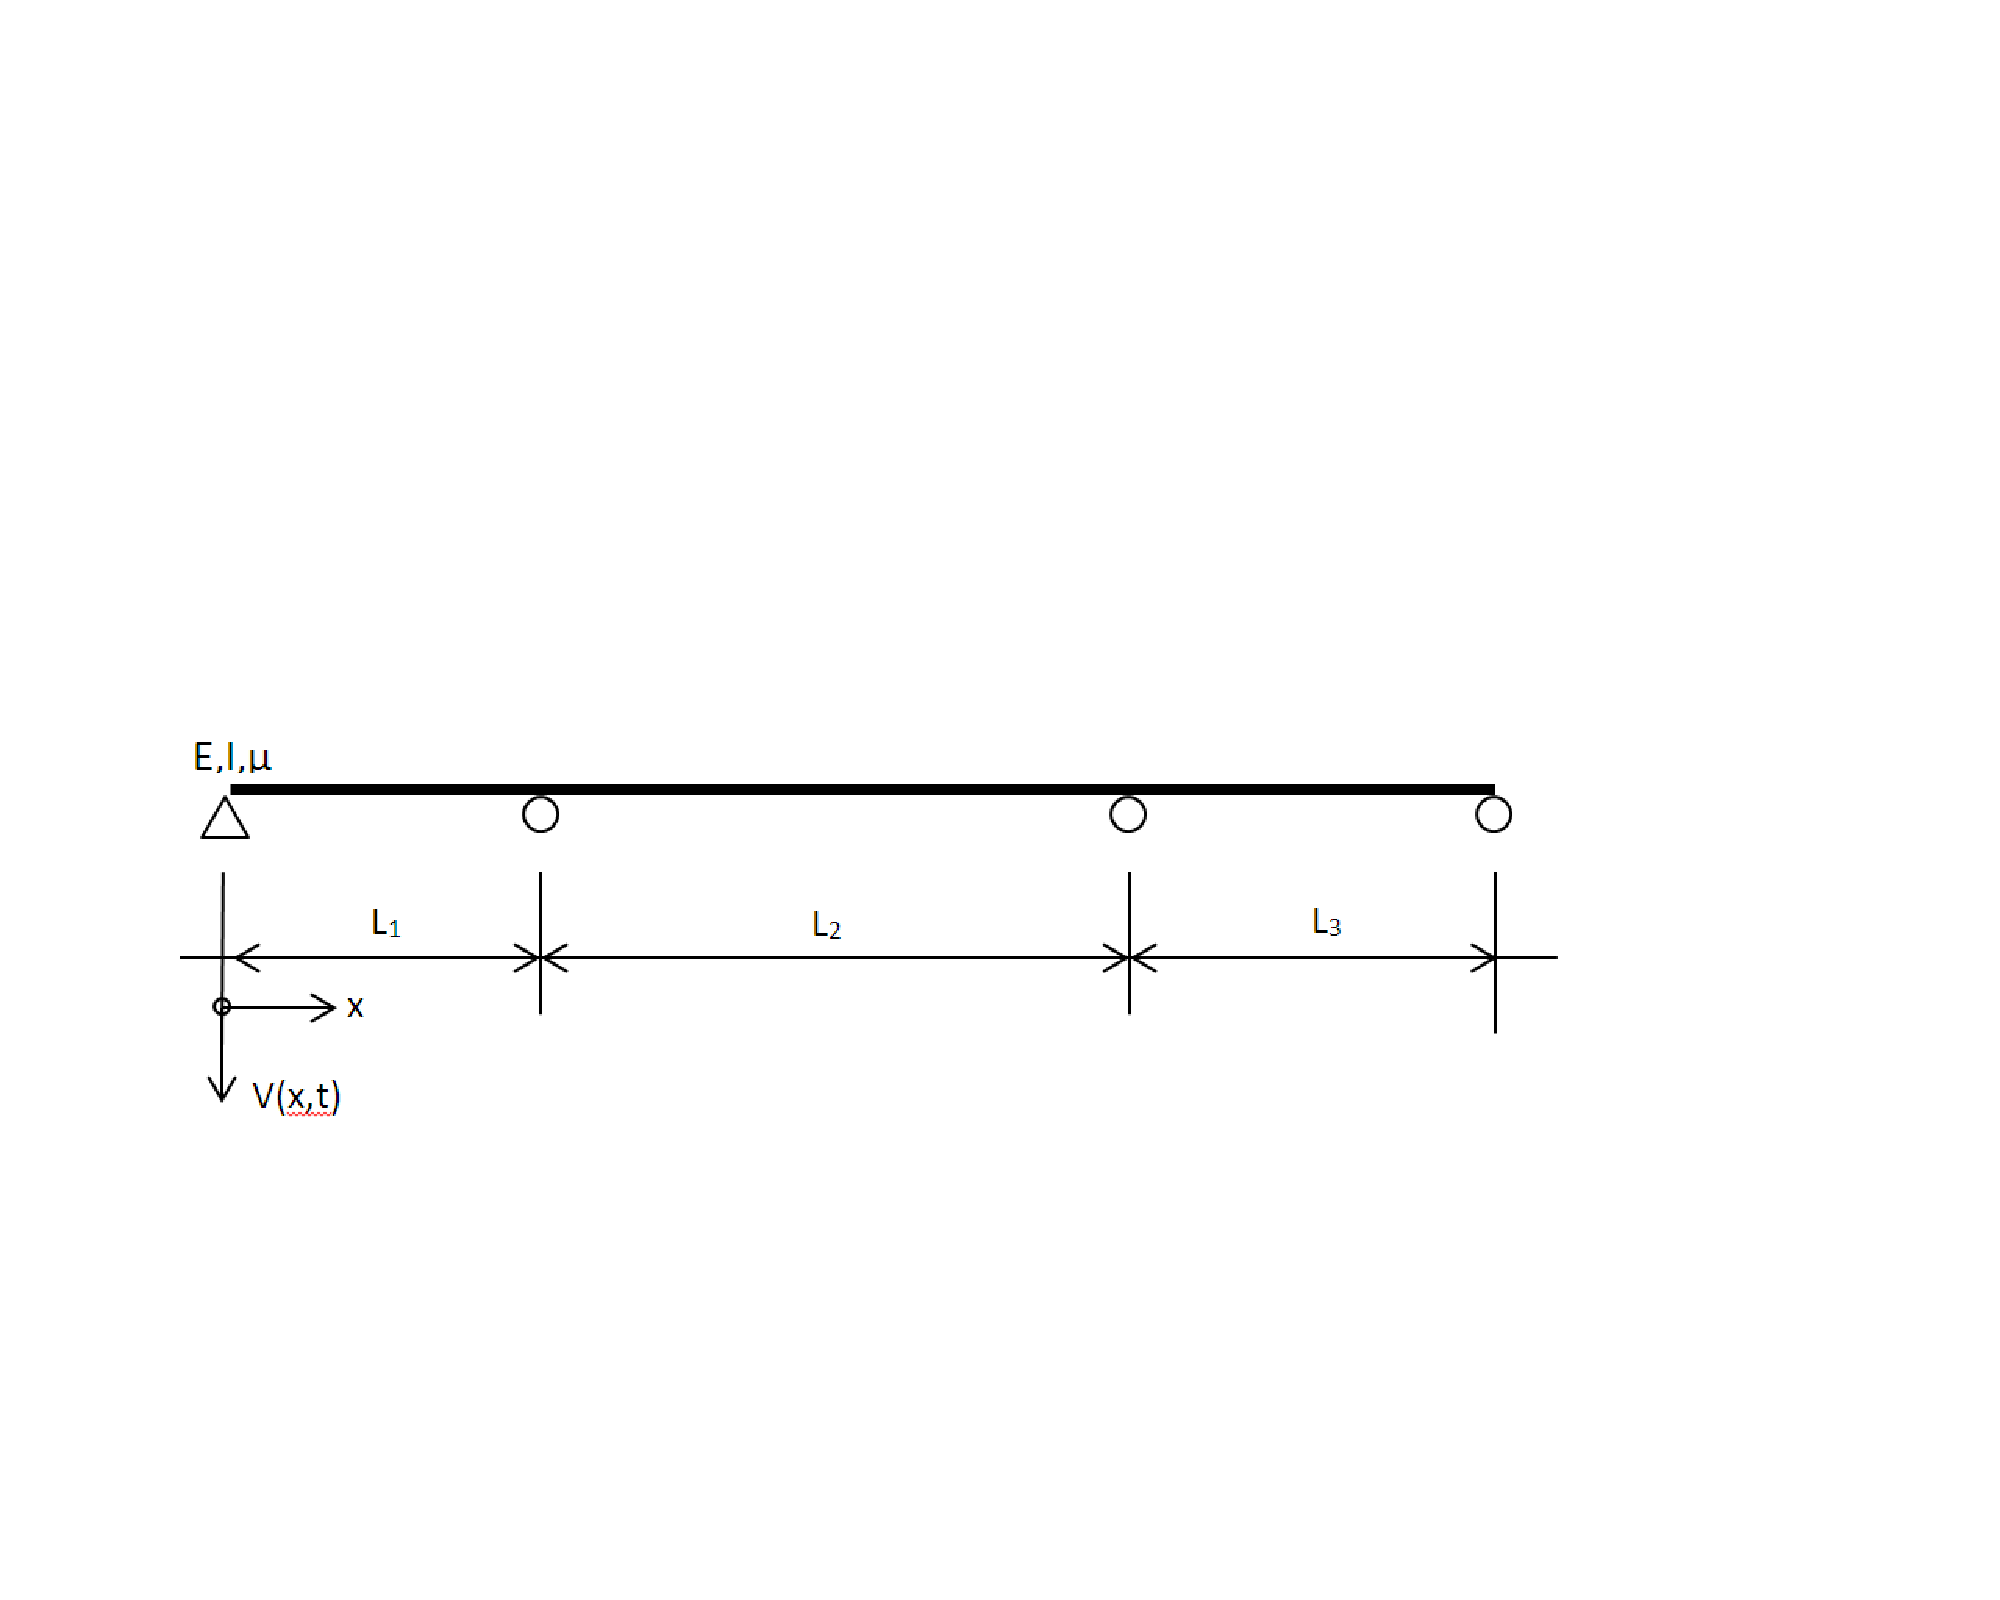
\includegraphics[width=0.8\textwidth]{continuousbeammodel.pdf}
	\caption{Continuous beam model}
	\label{fig:continuousbeammodel}
\end{figure}
	
\subsection{Complex systems}

\subsubsection{Trusses}

\subsubsection{Frames}

\subsubsection{Curved bars}

\subsection{High strength steel bridges}
The advantage of high strength steel bridges are

\begin{enumerate}
	\item High quality material
	\item Speed of construction
	\item Versatility
	\item Modification and repair
	\item Recycling
	\item Durability
	\item Aesthetics
\end{enumerate}

\cite{macdougall2004state}: Use of high-strength steels for bridge construction in Japan dates back to the 1960s. Several hundred bridges been constructed using 500MPa and 600MPa yield strength steel, and steel with a normal yield strength of 800 MPa has also been used on several projects. In Europe, a variety of high-strength steels with yield strength from 460MPa to 690MPa are available for bridge applications. European structural steel standard EN 10025: 2004 grade S460ML, which has a nominal yield strength of 460MPa, can be welded at room temperature for plate thickness up to 90mm and has a specified minimum Charpy V-notch(CVN) evergy of 27 J at -50$^\circ$C.

\section{Modelling of railway vehicles}
According to Newton's law, 2 basic load effects are produced by moving train: vertical forces due to vehicle weight, and inertia effects caused by vehicle acceleration. The loads on a railway bridge are very complex problems thus in engineering practice, loads are often simplified. But, the simplification depends on the purpose of the analysis. 

\subsection{Moving vertical forces model}
If the inertia effects are neglected, loads of the moving trains can be modelled as moving vertical forces. For example, load diagram for type TALGO trains is shown in Figure.\ref{fig:verticalmodel} proposed by \cite{uic}.

\begin{figure}[h]
	\centering
	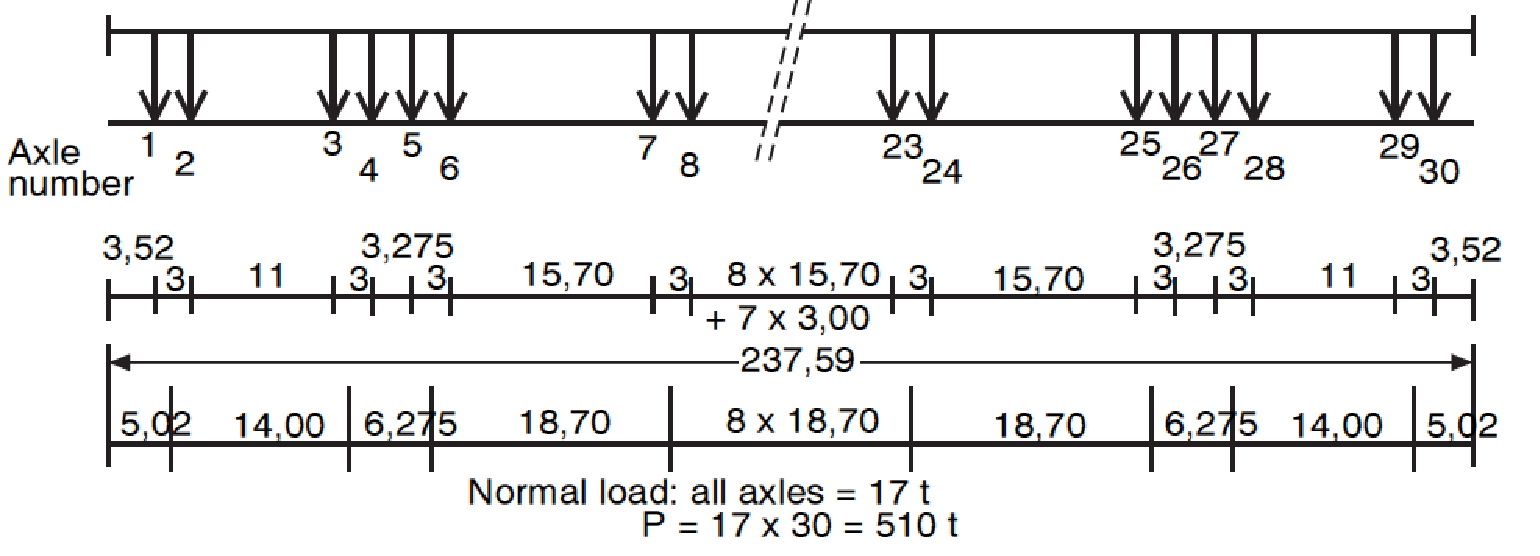
\includegraphics[width=0.8\textwidth]{verticalmodel.pdf}
	\caption{Moving vertical force model for TALGO trains}
	\label{fig:verticalmodel}
\end{figure}

\subsection{Advanced models}
Nowadays more and more models have been proposed to meet different requirements of railway bridge dynamic analysis. The complexity of these models differs from each other but they are all more complicated than moving vertical forces models. For example, vehicle-bridge interaction model takes vehicle suspension system into account, which gives an alternative for discovering resonance effects between bridge and the vehicle suspension systems. 

See Figure.\ref{fig:advancedmodel} for an example of advanced model.

\begin{figure}[p]
	\centering
	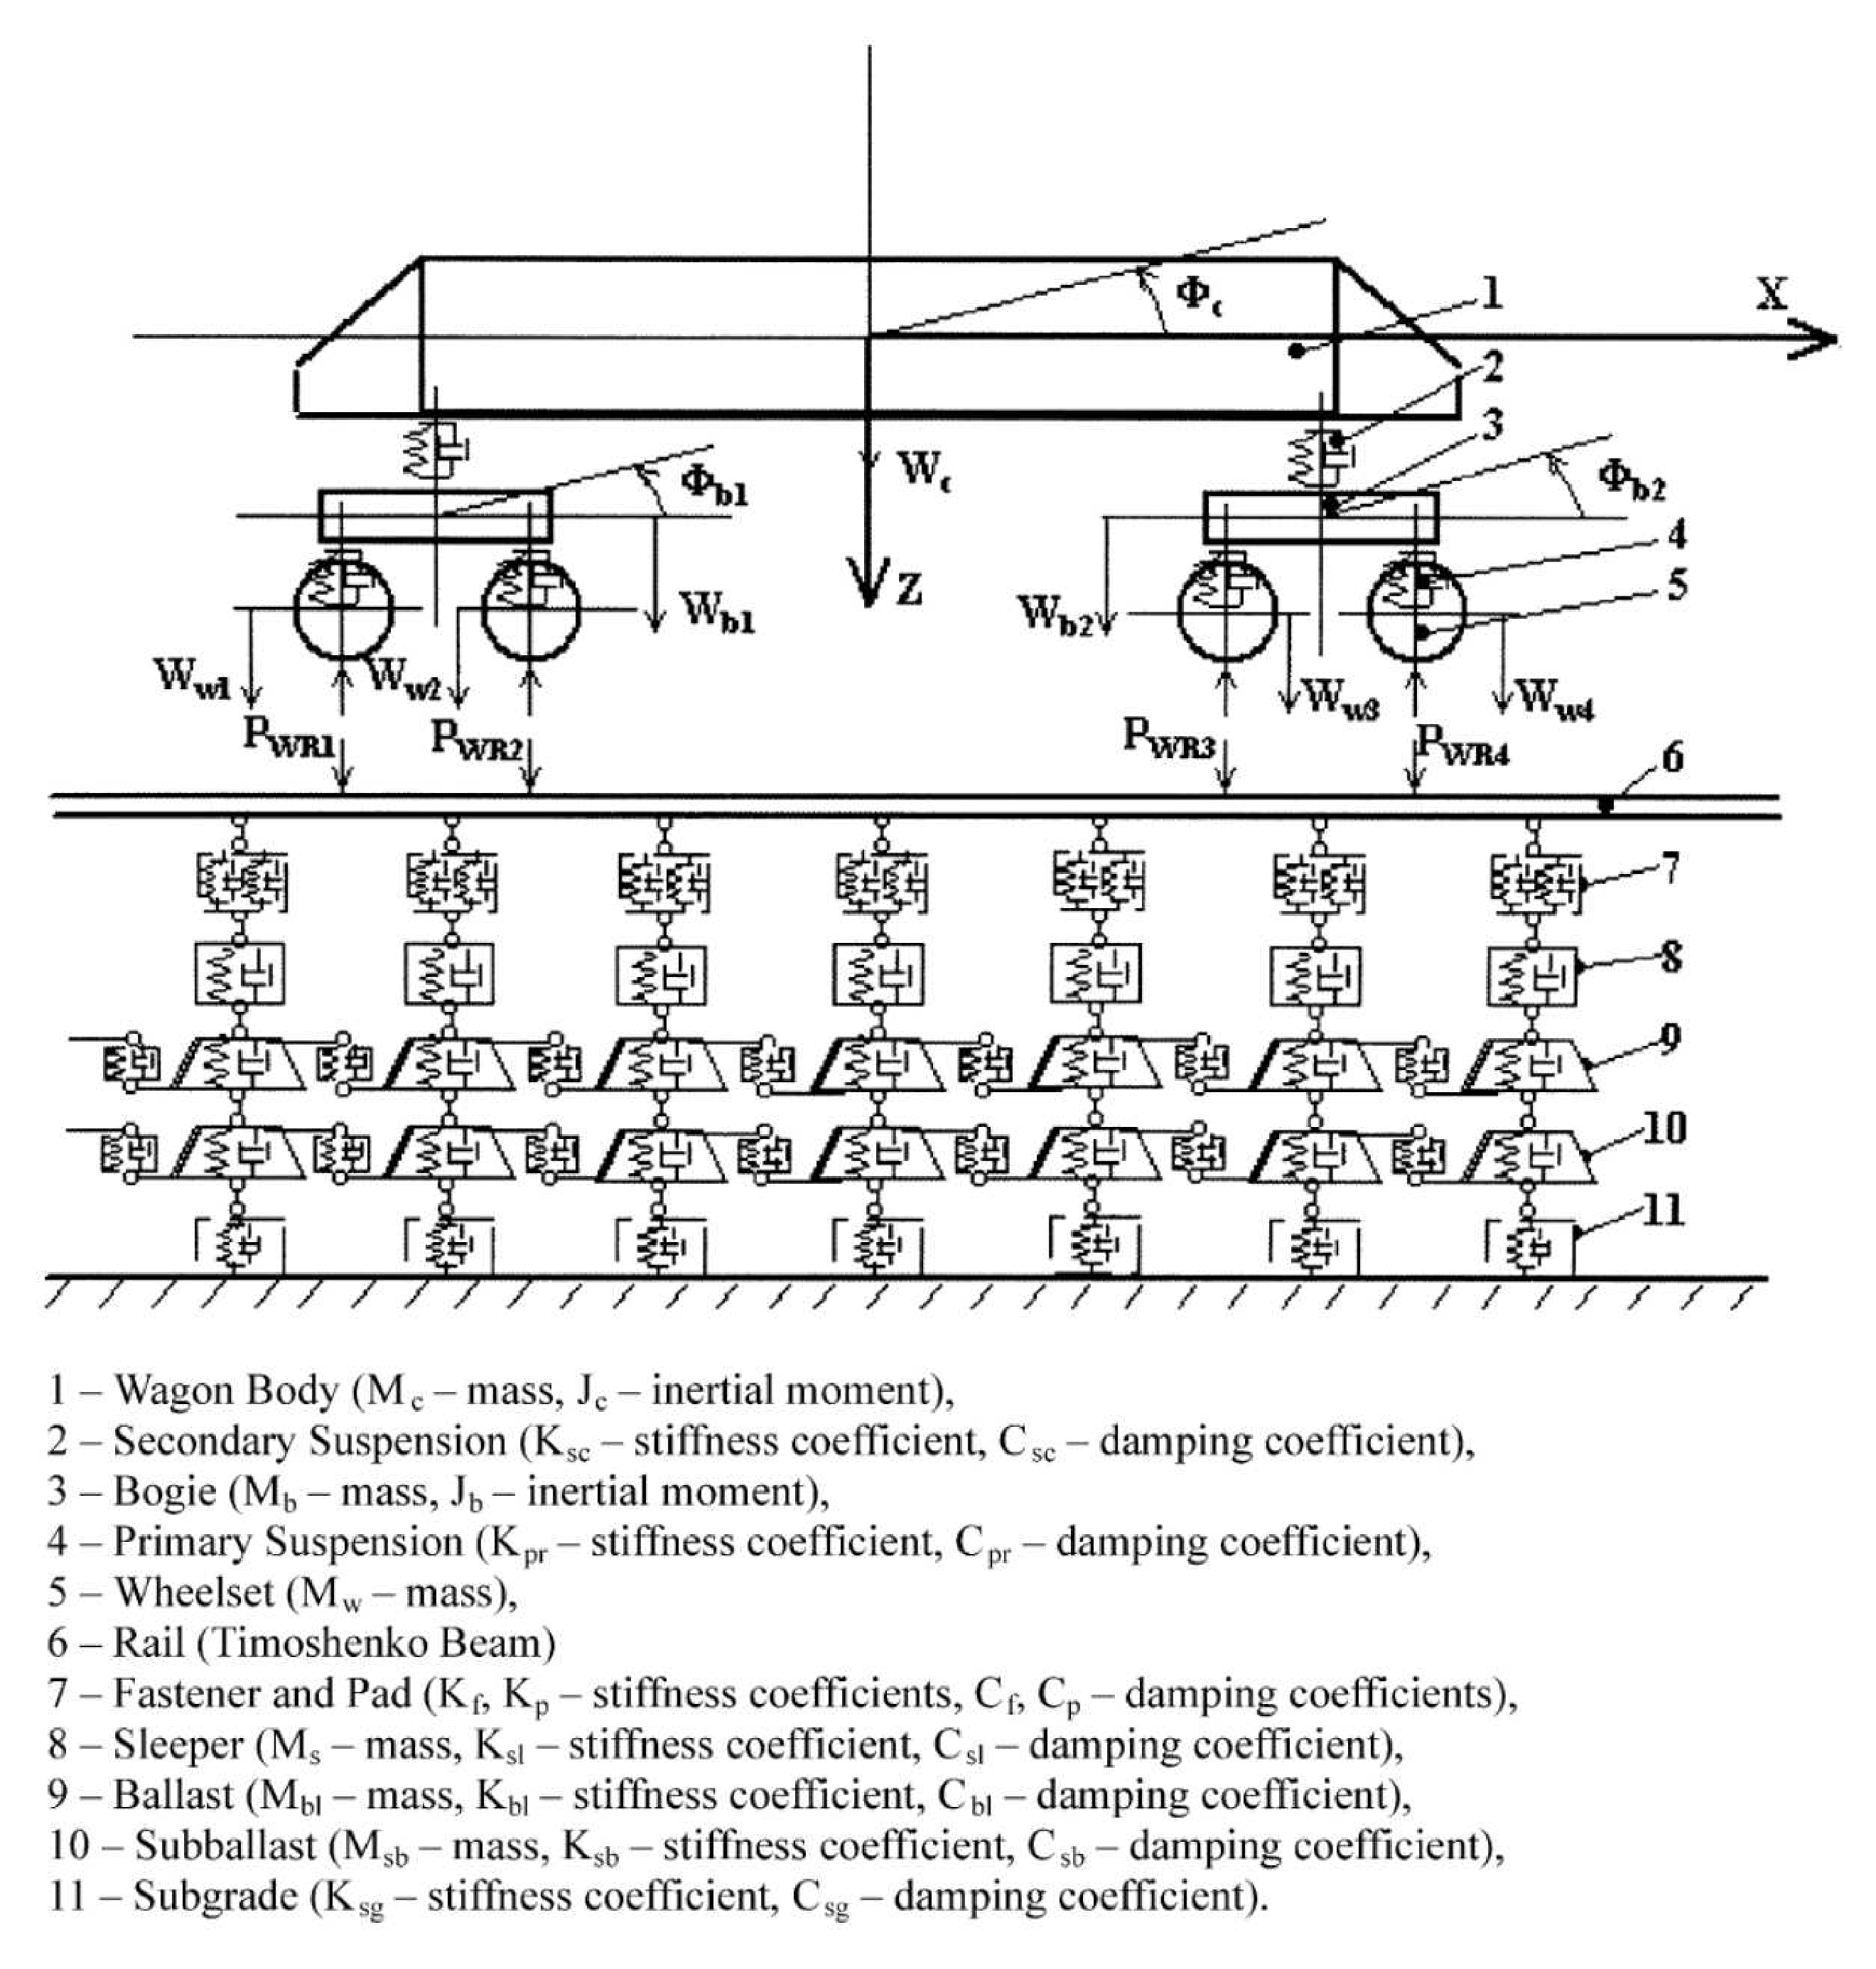
\includegraphics[width=0.8\textwidth]{advancedmodel.pdf}
	\caption{A dynamic model for the vertical interaction of the rail track and wagon system. Proposed in \cite{sun2002dynamic}}
	\label{fig:advancedmodel}
\end{figure}


\subsection{Models proposed in Eurocodes}

See Chapter~\ref{sec:train-models}

\section{Track model}
Proposed in \cite[A.6.1.3]{uic}, the track is represented by Timoshenko beam elements for the rails and takes account of the rail/sleeper fastening characteristics as well as the ballast(if one exists).

\textit{``A sleeper is generally represented by two beam elements, with two covering the rail and one used for the deck. Sleepers and ballast are modelled as concentrated masses. They are linked to the nodes of the rail and the bridge by a parallel spring and damper system. The track can be modelled to any length on both side of the bridges, where the stiffening effect of the bridge has to be taken into account. The effects of track distribution are not considered. Each vehicle is able to absorb the kinetic energy of the bridge and it is for this reason that, at resonance, the deflections and accelerations of the bridge obtained with this model are lower than those obtained with a live load diagram."}

The most complete model for analysing train/track/bridge interaction is shown in Figure

\begin{figure}[h]
	\centering
	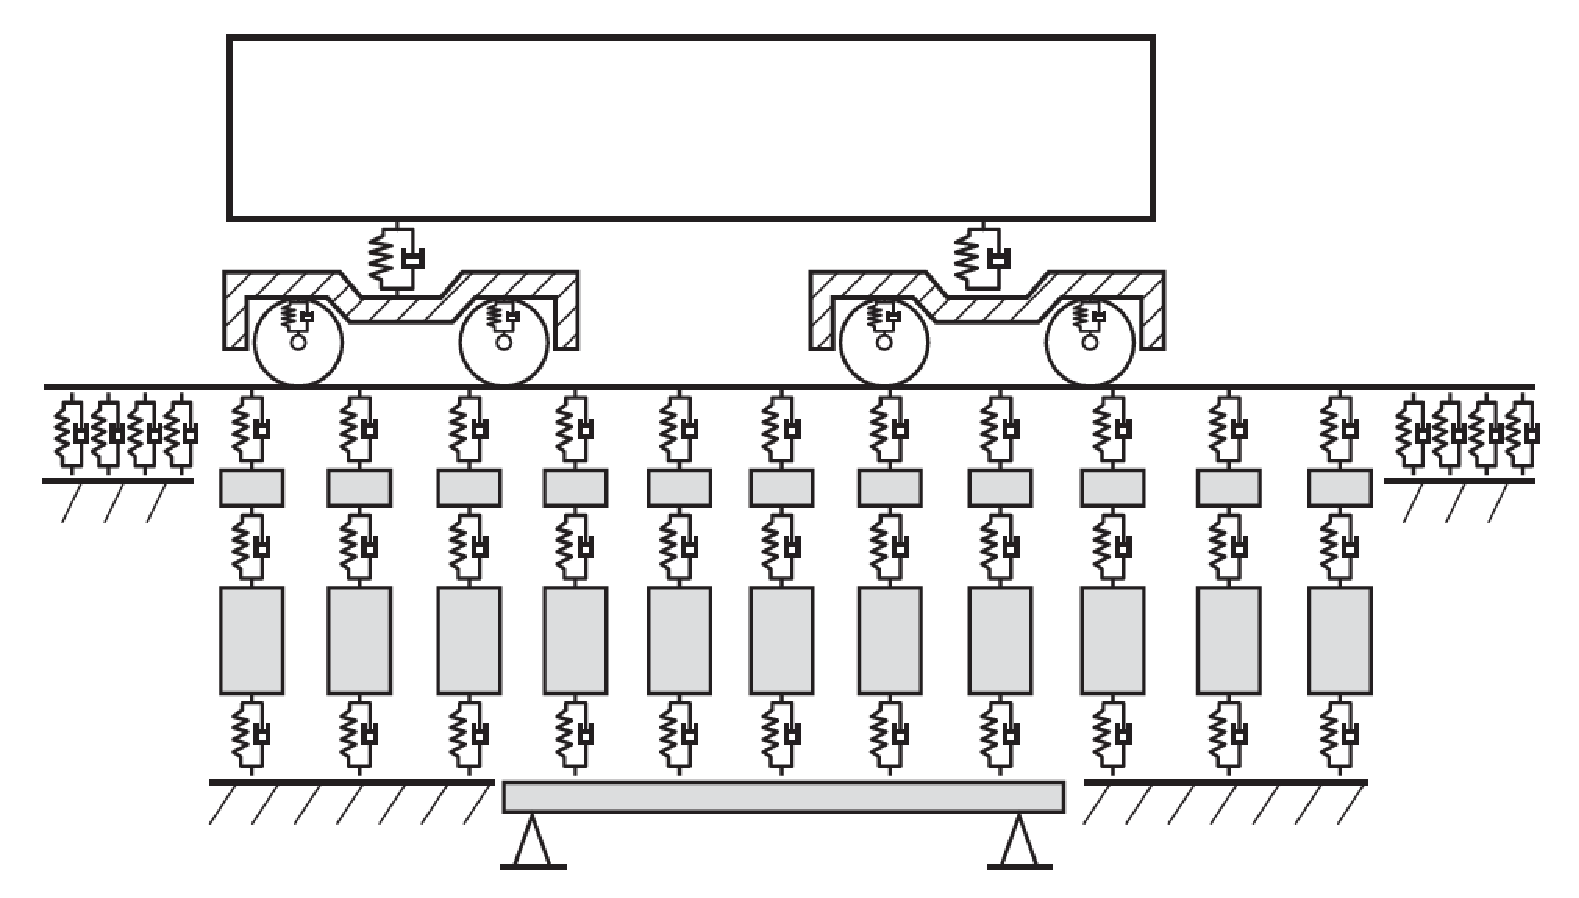
\includegraphics[width=0.8\textwidth]{trackmodel.pdf}
	\caption{Diagram of the dynamic train-track-bridge model. Extracted from \cite[Fig. 15]{uic}}
	\label{fig:trackmodel}
\end{figure}


\section{General design principles and procedures concerning railway bridge dynamics proposed by Eurocodes } \label{designprocedures}


\subsection{Requirements for railway bridge verification}
\cite{EC0} propose following requirements


\begin{enumerate}
	\item Checks on bridge deformations shall be performed for traffic safety purposes for the following items:
	\begin{enumerate}[-]
		\item vertical accelerations of the deck
		\item vertical deflection of the deck throughout each span
		\item unrestrained uplift at the bearings(to avoid premature bearing failure)
		\item vertical deflection of the end of the deck beyond bearings(to avoid destabilising the track, limit uplift forces on rail fastening systems and limit additional rail stresses) 
		\item twist of the deck measured along the centre line of each track on the approaches to a bridge and across a bridge(to minimise the risk of train derailment)
		\item rotation of the ends of each deck about a transverse axis or the relative total rotation between adjacent deck ends(to limit additional rail stresses, limit uplift forces on rail fastening systems and limit angular discontinuity at expansion devices and switch blades)
		\item longitudinal displacement of the end of the upper surface of the deck due to longitudinal displacement and rotation of the deck end(to limit additional rail stresses and minimise disturbance to track ballast and adjacent track formation)
		\item horizontal transverse deflection(to ensure acceptable horizontal track radii)
		\item horizontal rotation of a deck about a vertical axis at ends of a deck (to ensure acceptable horizontal track geometry and passenger comfort)
		\item limits on the first natural frequency of lateral vibration of the span to avoid the occurrence of resonance between the lateral motion of vehicles on their suspension and the bridge
	\end{enumerate}
	\item Checks on bridge deformations should be performed for passenger comfort, i.e. vertical deflection of the deck to limit coach body acceleration in accordance with A2.4.4.3\cite{EC0}
	\item The limits given in A2.4.4.2 and A2.4.4.3\cite{EC0} take into account the mitigating effects of track maintenance (for example to overcome the effects of the settlement of foundations, creep, etc.) 
\end{enumerate}

\subsection{Conceptual check}
The conceptual check is to help designers avoid unsafe designs in conceptual stage. Once the bridge type and rough geometry is sketched, designers can easily know whether the bridge would have dynamic problem in the future. 

For example, in  \cite[cl.8.7.4]{calgaro2010designers}, it is stated that if the bridge meets criteria ~\ref{cr:nocheck} , no dynamic analysis in necessary. 

\begin{equation}
	\label{cr:nocheck}
	V>200km/h \quad \delta_{dyn} \leq \text{ value given by the dynamic study, but }\delta_{stat}\leq L/2600
\end{equation}

On the other hand, no other conceptual check criterion is given for train speed under 200km/h. Since there is higher possibility that, for bridges with span larger than 100m, they will have resonance with the normal trains. 

\subsection{Logic diagram}

This logic diagram is used to determine whether a dynamic analysis is required, as shown in Figure~\ref{fig:logicdiagram}, is represented in \cite{EC12} Chapter 6.4 Dynamic Effects, where $V [Km/h]$ is the Maximum Line Speed at the site, $L [m]$, the span length, $n_0 [Hz]$, the first nature frequency under permanent loads, $n_T$, the first natural torsional frequency for the same load, $v [m/s]$ the maximum nominal speed and finally $(v/n_0)_{lim}$, as given in Annex F of EN1991-2. The frequency first of vibration, $n_0$, must be within the limits established in figure~\ref{fig:frequencylimit}.

Checking through the logic diagram is regarded as first step is because designers can try to avoid designs that will be required to be dynamic analysed in the very beginning of the designing phase. 

The upper limit (1) is defined as

\begin{equation}
	n_0=94,76L^{-0,748}
\end{equation}

and the lower limit (2) as:

\begin{equation}
	n_0= \{ \begin{array}{ll}
	80/L & \mbox{for $4m\leq L \leq 20m$} \\
	94,76L^{-0,748} & \mbox{for $20m\leq L \leq 100m$}
\end{array} 
\end{equation}

\begin{figure}[h]
\centering
	\begin{subfigure}[b]{0.45\textwidth}
    	\centering
    	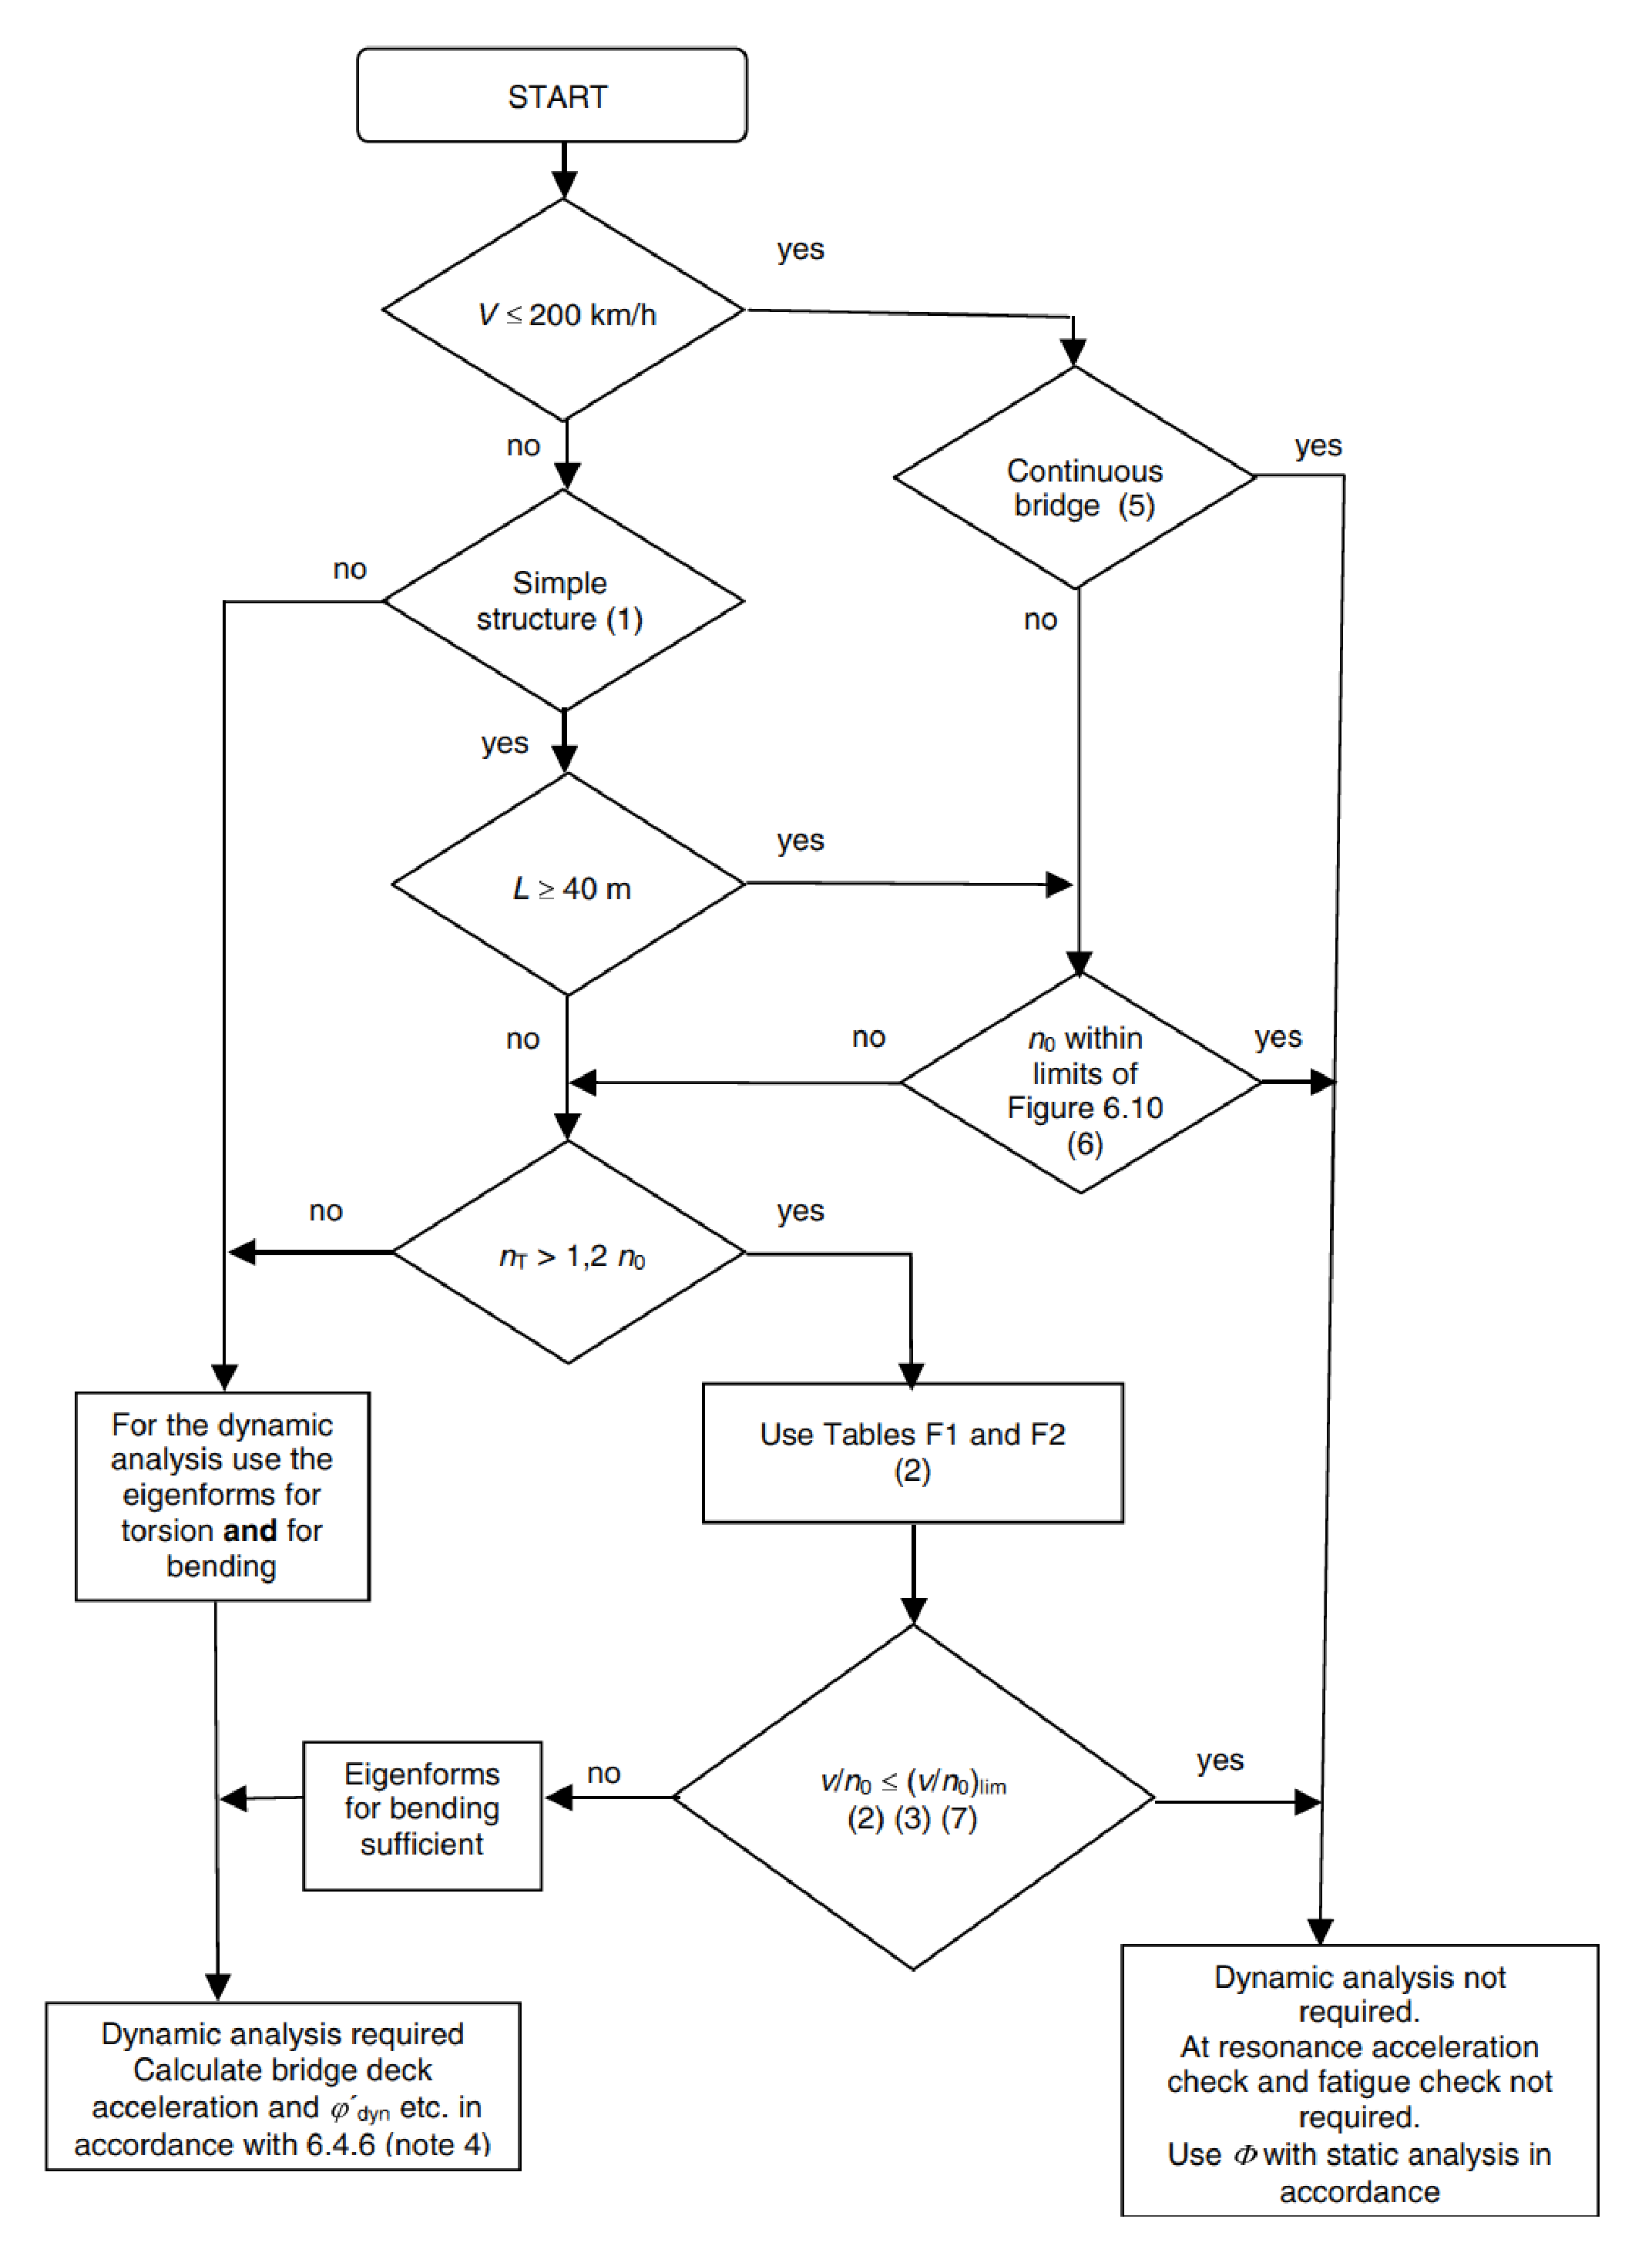
\includegraphics[width=\textwidth]{logicdiagram.pdf}
    	\caption{Flow chart for determining whether a dynamic analysis is required. Extracted from EN1991-2\cite{EC12}}
    	\label{fig:logicdiagram}
	\end{subfigure}
	\begin{subfigure}[b]{0.45\textwidth}
    	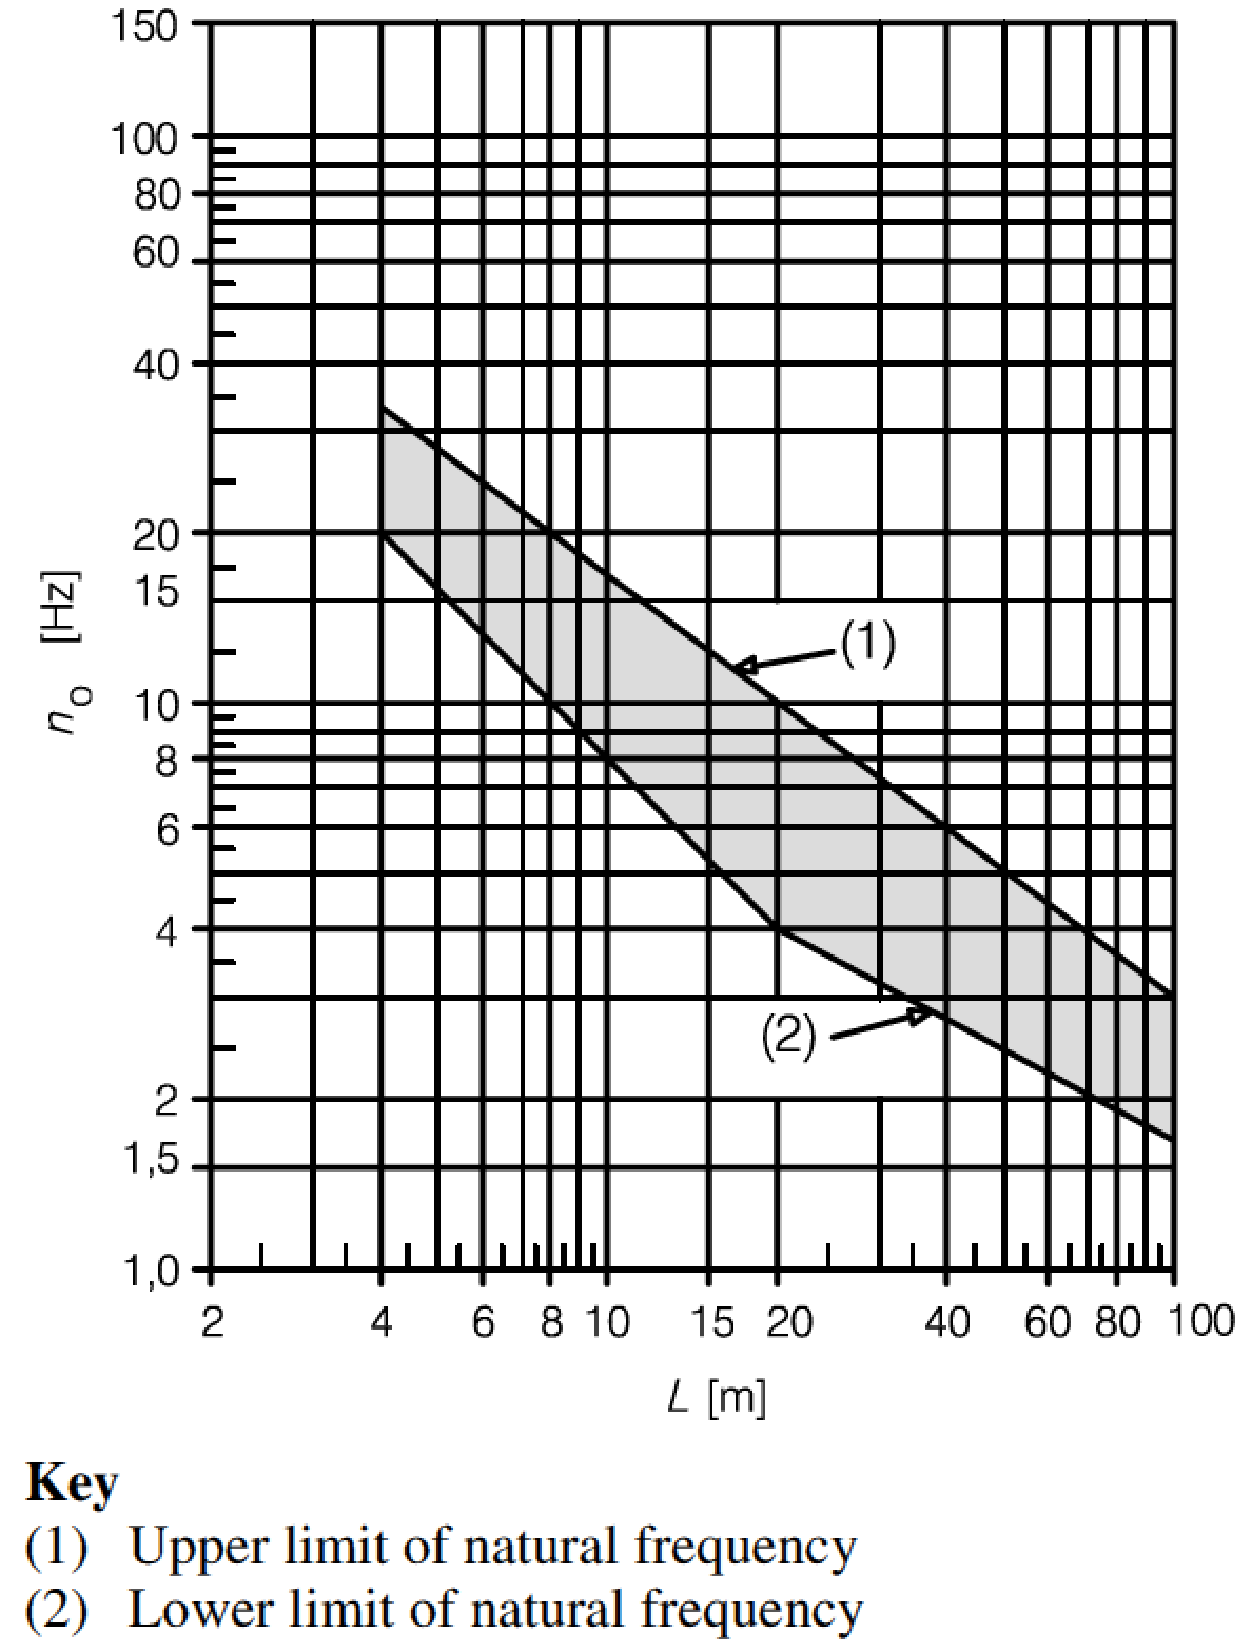
\includegraphics[width=\textwidth]{frequencylimit.pdf}
    	\caption{Limits for bridge natural frequencies, $n_0 [Hz]$, as a function $L [m]$. Extracted from EN1991-2\cite{EC12}.}
    	\label{fig:frequencylimit}
	\end{subfigure}
\caption{Logic diagram for determining whether dynamic analyses are necessary, extracted from \cite[6.4.4]{EC12}}
\label{logicandlimit}
\end{figure}

\subsection{Train models}\label{sec:train-models}
According to NEN 1991-2\cite{EC12} and Designers Guide\cite{calgaro2010designers} Rail traffic actions are defined by means of load models, Four models of railway loading are given:
\begin{enumerate}[$\bullet$]
	\item LM71 and LM SW/0(for continuous bridges) to represent normal rail traffic on mainline railways (passenger and heavy freight traffic)
	\item SW/2 to represent abnormal loads or waggons
	\item LM 'unloaded train' to represent the effect of an unloaded train
	\item LM HSLM (comprising HSLM-A and HSLM-B) to represent the loading from passenger trains at speeds exceeding 200km/h.
\end{enumerate}

\subsubsection{Load Model 71}
LM71 represents the static effect of vertical loading due to normal rail traffic.

The load arrangement and the characteristic values for vertical loads have to be taken as shown in Figure.~\ref{lm71}

The actions listed below, associated with LM71, have to be multiplied by factor $ \alpha $:

\begin{enumerate}[-]
	\item equivalent vertical loading for earthworks and earth pressure effects
	\item centrifugal forces
	\item nosing force (multiplied by $ \alpha $ for $ \alpha\geq 1 $ only)
	\item traction and braking forces
	\item derailment actions for accidental design situations
	\item Load Model SW/0 for continuous span bridges
\end{enumerate}

\textit{For international lines, it is recommended that a value of $ \alpha \geq 1.0 $ is adopted. But this freedom of choice of the factor $ \alpha $ could lead to a non-uniform railway network in Europe. Therefore in UIC Code 702\textsuperscript{4} $ \alpha=1.33 $ is generally recommended for all new bridges constructed for the international freight network, but not compulsory}. 

\begin{figure}[h]
	\centering
	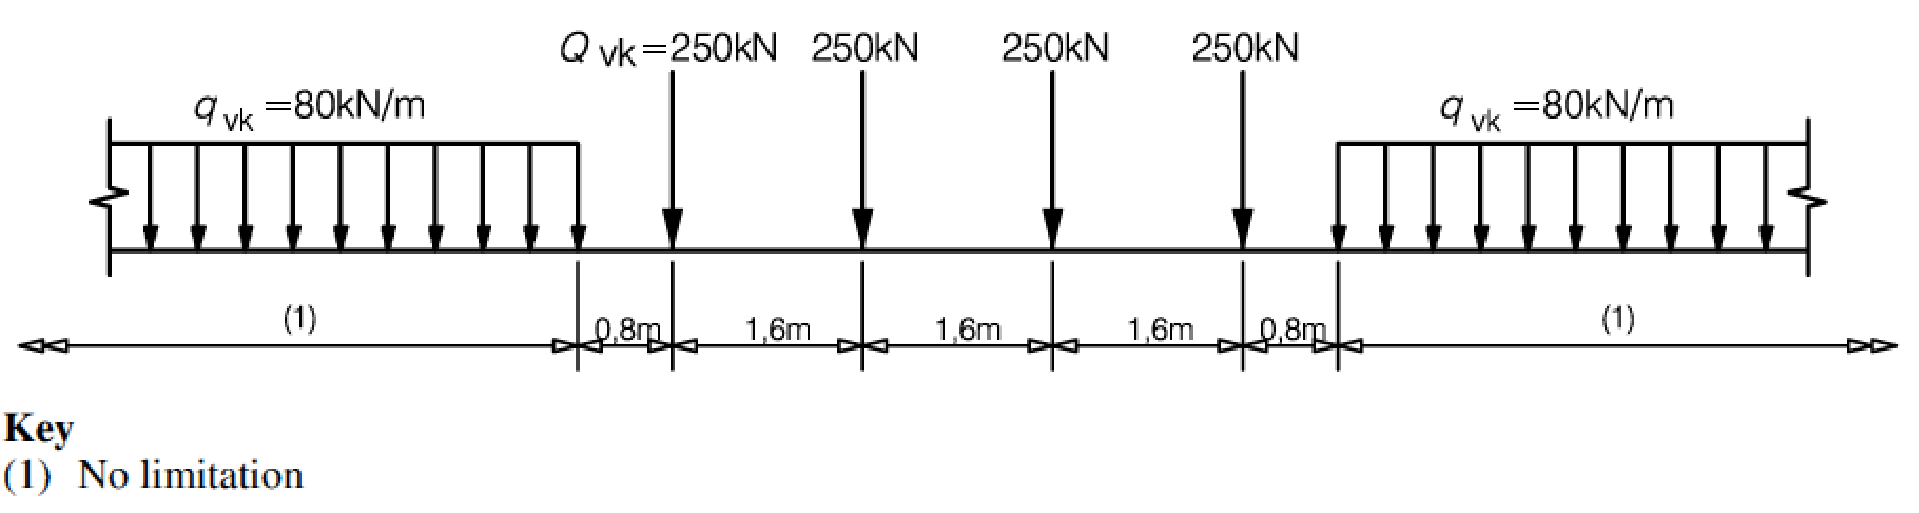
\includegraphics[width=0.8\textwidth]{lm71.pdf}
	\caption{Load Model 71 and characteristic values for vertical loads. Extracted from EN1991-2\cite{EC12}}
	\label{lm71}
\end{figure}

\subsubsection{Load Models SW/0 and SW/2}
Load Models SW/0 represents the static effect of vertical loading due to normal rail traffic on continuous beams.

Load Model SW/2 represents the static effect of vertical loading due to heavy abnormal rail traffic. 

The load arrangement is as shown in Figure.~\ref{lmsw}, with the characteristic values of the vertical loads according to Table.\ref{tab:sw}

\begin{figure}[h]
	\centering
	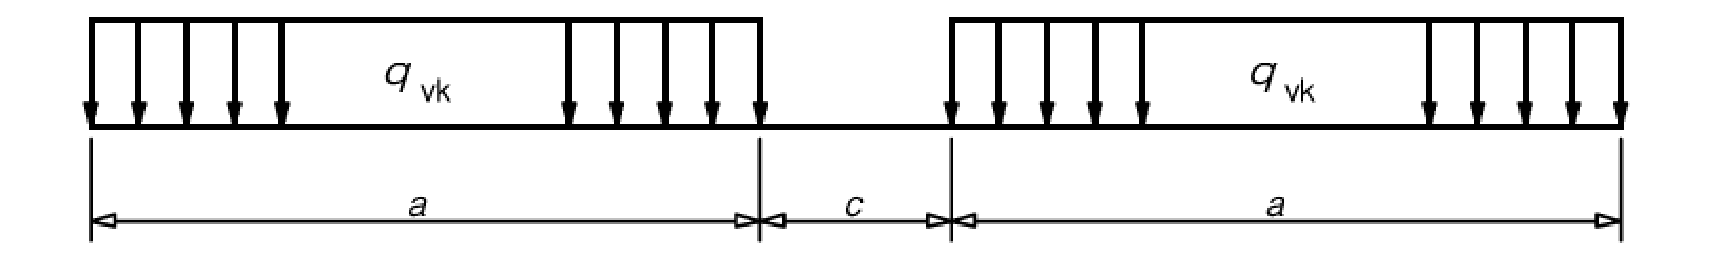
\includegraphics[width=0.8\textwidth]{lmsw.pdf}
	\caption{Load Models SW/0 and SW/2.. Extracted from EN1991-2\cite{EC12}}
	\label{lmsw}
\end{figure}

\begin{table}[h]
	\centering
	\begin{tabular}{llll}
		\hline
		Load model & $ q_{vk} (kN/m) $ & $ a (m) $ & $ c (m) $ \\
		\hline
		SW/0 & 133 & 15.0 & 5.3\\
		SW/2 & 150 & 25.0 & 7.0\\
		\hline
	\end{tabular}
	\caption{Characteristic values for vertical loads for Load Models SW/0 and SW/2}
	\label{tab:sw}
\end{table}

\subsubsection{Load Model 'unloaded train'}
From some specific verification purposes a specific load model is used, called 'unloaded train'. The Load Model 'unloaded train' consists of a vertical uniformly distributed load with a characteristic value of 10.0kN/m.

\subsubsection{Load Models SHLM}
Load Models HSLM comprises two separate universal \textit{high-speed} trains with variable coach lengths. In order to ensure that they deliver dynamic behaviour with regards to current and future train traffic, bridges should be calculated using the Universal Dynamic Train(HSLM) consisting of HSLM-A and/or HSLM-B. These are defined as follows:

\begin{enumerate}[$ \bullet $]
	\item For the definition of train HSLM-A, a set of ten reference trains A1 to A10: see Figure.~\ref{fig:hslma} and Table.~\ref{tab:hslma} below.
	\item For the definition of train HSLM-B: See Figure.~\ref{fig:hslmbdiagram} and `\ref{fig:hslmbtable} below
\end{enumerate}

\begin{figure}[h]
	\centering
	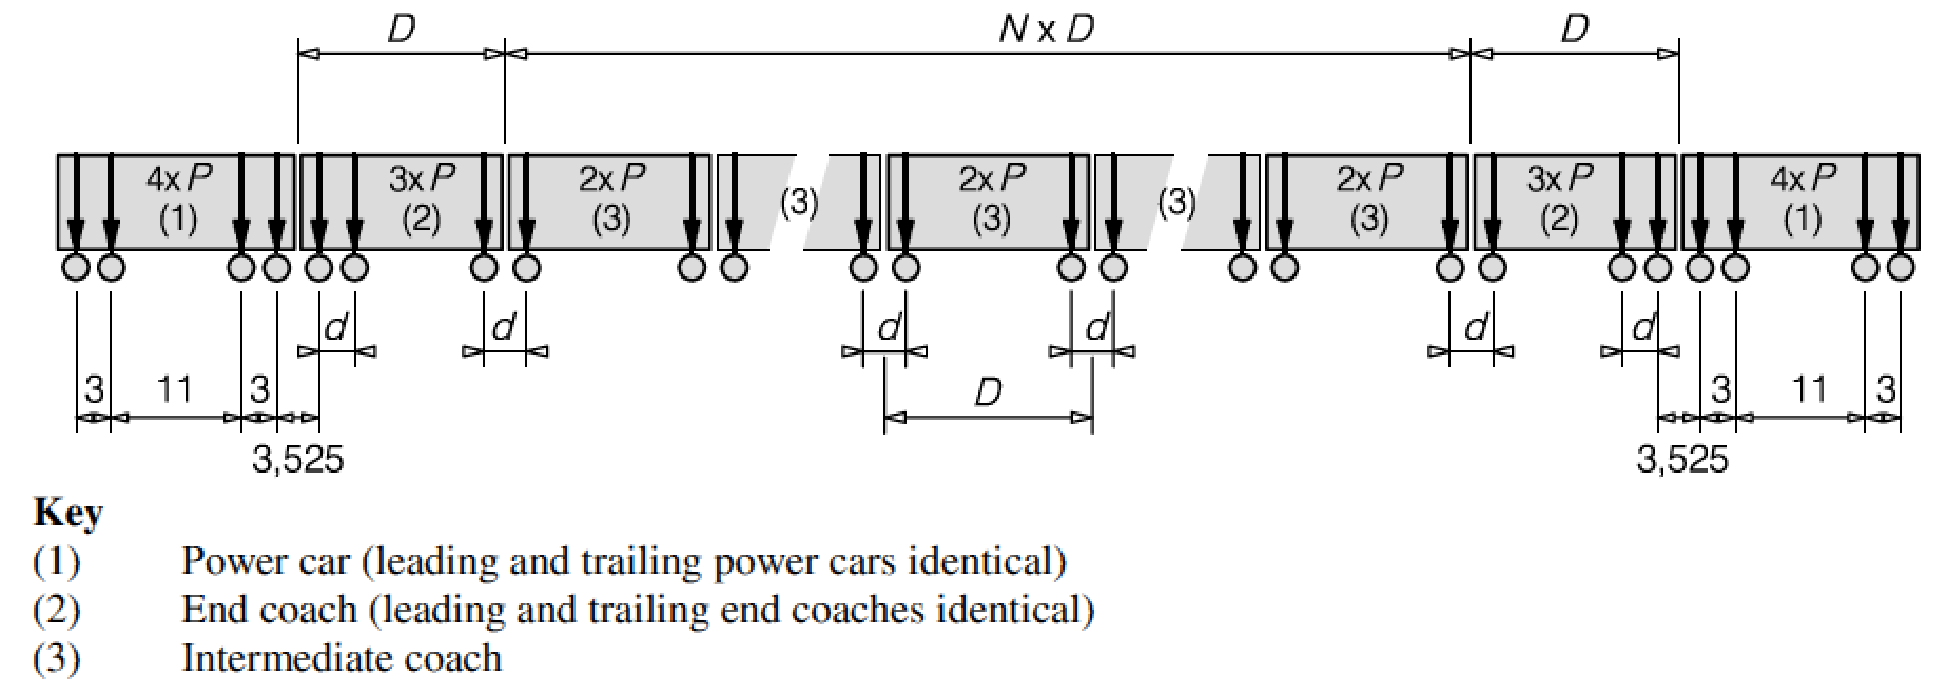
\includegraphics[width=0.8\textwidth]{hslma.pdf}
	\caption{Diagram of Universal Dynamic Train HSLM-A. Extracted from EN 1991-2\cite{EC12}}
	\label{fig:hslma}
\end{figure}

\begin{table}[h]\footnotesize
	\centering
	\begin{tabular}{p{2cm}p{2cm}p{2cm}p{2cm}p{2cm}}
		\hline
		Universal train & Number of intermediate coaches, $ N $ & Coach length $ D(m) $ & Bogie axle spacing $ d (m) $ & Point force $ P (kN) $ \\
		\hline
		A1 & 18 & 18 & 2.0 & 170 \\
		A2 & 17 & 19 & 3.5 & 200 \\
		A3 & 16 & 20 & 2.0 & 180 \\
		A4 & 15 & 21 & 3.0 & 190 \\
		A5 & 14 & 22 & 2.0 & 170 \\
		A6 & 13 & 23 & 2.0 & 180 \\
		A7 & 13 & 24 & 2.0 & 190 \\
		A8 & 12 & 25 & 2.5 & 190 \\
		A9 & 11 & 26 & 2.0 & 210 \\
		A10 & 11 & 27 & 2.0 & 210 \\			
		\hline		
	\end{tabular}
	\caption{HSLM-A, definition of ten trains. Extracted from EN1991-2\cite{EC12}}
	\label{tab:hslma}
\end{table}

\begin{figure}[h]
	\centering
	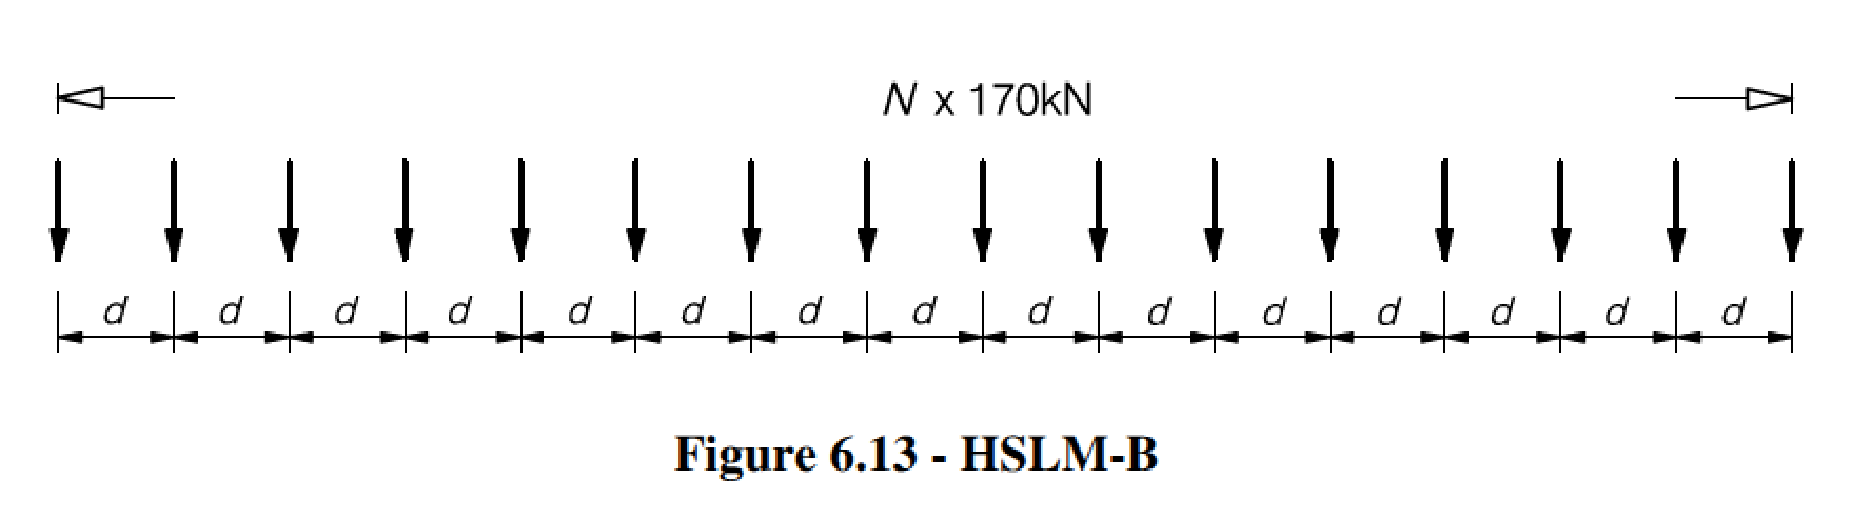
\includegraphics[width=0.8\textwidth]{hslmb.pdf}
	\caption{Diagram of Universal Dynamic Train HSLM-B. Extracted from EN 1991-2\cite{EC12}}
	\label{fig:hslmbdiagram}
\end{figure}

\begin{figure}[h]
	\centering
	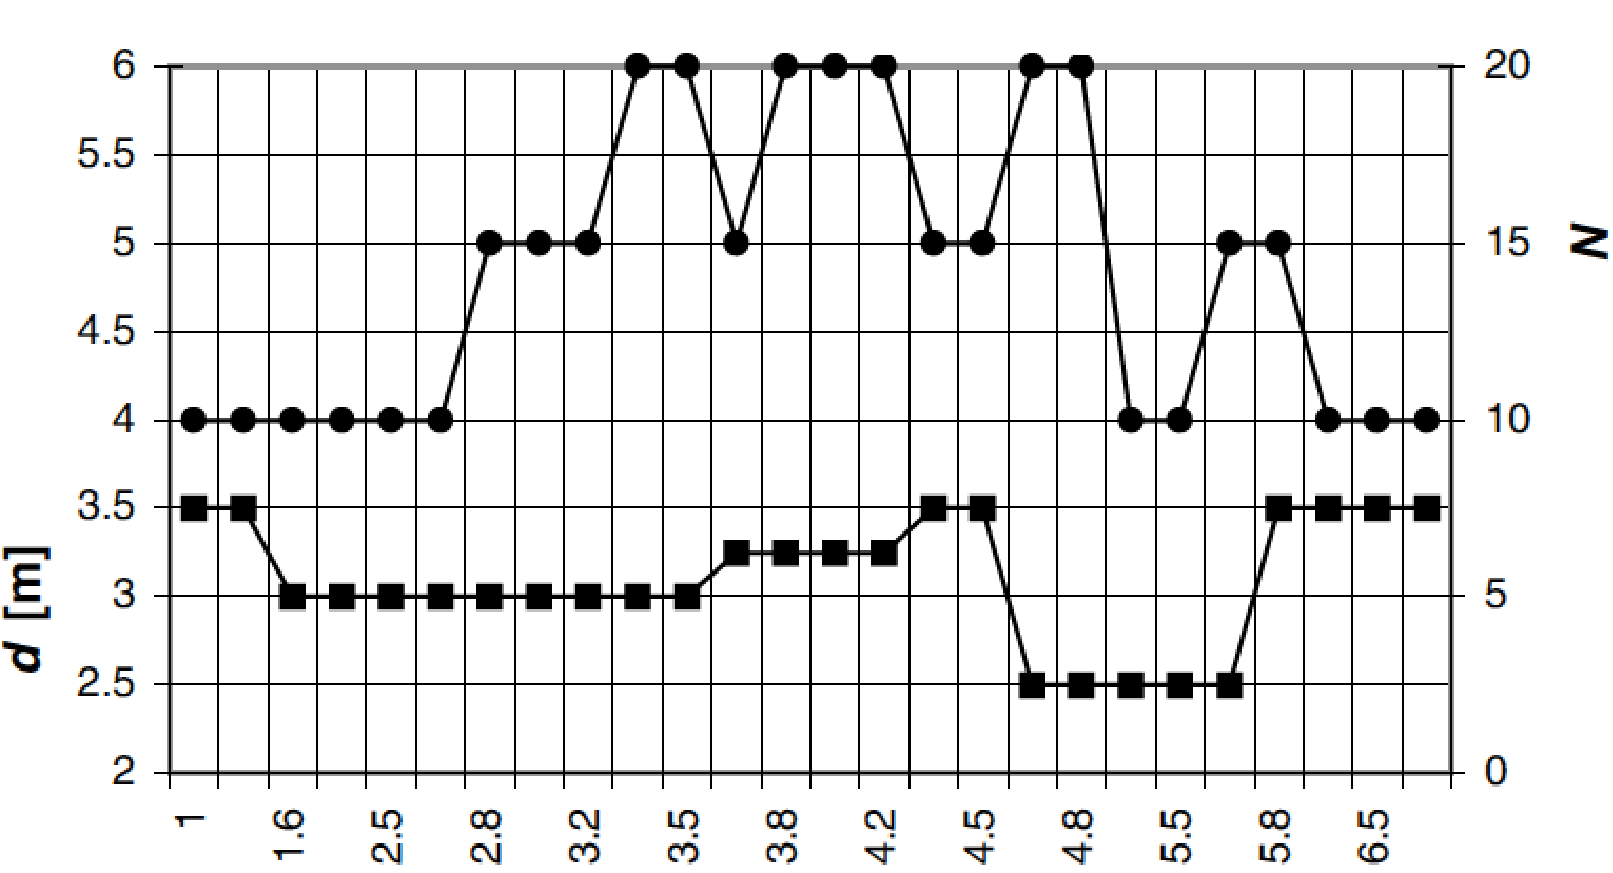
\includegraphics[width=0.8\textwidth]{hslmb2.pdf}
	\caption{Universal Dynamic Train HSLM-B. Extracted from EN 1991-2\cite{EC12}}
	\label{fig:hslmbtable}
\end{figure}

This Load Model comprises $ N $ number of point forces of 170kN at regular spacing $ d(m) $ (\ref{fig:hslmbdiagram}) where $ N $ and $ d $ are defined in Figure.~\ref{fig:hslmbtable}

Table.~\ref{hslmapplication} illustrates how HSLM-A and HSLM-B are applied and indicates the train to be used for dynamic bridge calculations.

\begin{table}[h] \scriptsize
	\begin{tabular}{lll}
		\hline
		Structural configuration & \multicolumn{2}{c}{Span} \\
		& $ L<7m $ & $ L\geq 7m $ \\
		\hline
		Simply supported span & HSLM-B & HSLM-A \\
		Continuous structure or Complex Structure & Trains A1 to A10 inclusive & Trains A1 to A10 inclusive\\
	\end{tabular}
	\caption{Application of HSLM-A and HSLM-B. Data extracted from EN 1991-2\cite{EC12}}
	\label{hslmapplication}
\end{table}

\subsection{Dynamic factor}\label{sec:dynamicfactor}
The dynamic factor $ \Phi $ takes account of the dynamic magnification of stress and vibration effects in the structure but does not take account of resonance effects.

Generally the dynamic factor $ \varPhi $ is taken as either $ \varPhi_2 $ or $ \varPhi_3 $ according to the quality of track maintenance as follows:

\begin{enumerate}[(a)]
	\item For Carefully maintained track: 
		\begin{equation}
			\varPhi_2=\dfrac{1.44}{\sqrt{L_\varPhi}-0.2}+0.82 \quad with1.00\leq \varPhi_2\leq 1.67
		\end{equation}
	\item For track with standard maintenance:
		\begin{equation}
			\varPhi_3=\dfrac{2.16}{\sqrt{L_\varPhi}-0.2}+0.73 \quad with 1.00\leq \varPhi_3\leq 2.0
		\end{equation}\\
	where $ L_\varPhi $ is the `determinant' length (length associated with $ \varPhi $ ) in metres as defined in Table 6.2, EN1991-2\cite{EC12}.
\end{enumerate}

\subsection{Static analysis}
A static analysis shall be carried out with the load models defined in Section Load Models(LM71 and where required Load Models SW/0 and SW/2). The result shall be multiplied by the dynamic factor $ \Phi $ (and if required multiplied by $ \alpha $)

\subsection{Bridge parameters}
In designers' guide\cite{calgaro2010designers}, bridge parameters on dynamic effects are discussed.

\subsubsection{Structural damping}
Structural damping is a key parameter in dynamic analysis. The magnitude of the vibrations depends heavily on structural damping, especially in proximity to resonance.

\subsubsection{Mass of the bridge}
Maximum dynamic effects occur at resonance peaks, where a multiple of the load frequency coincides with the natural frequency of the structure. Underrating the mass will lead to over-estimation of the natural frequency of the structure and of the speed at which resonance occurs.

\subsubsection{Stiffness of the bridge}
Maximum dynamic load effects are likely to occur at resonant peaks when a multiple of the frequency of loading and a natural frequency of the structure coincide. Any overestimation of bridge stiffness will overestimate the natural frequency of the structure and speed at which resonance occurs; it provides conservative results.

\subsection{Dynamic analysis}
EN 1991-2\cite{EC12} doesn't specify the method of dynamic analysing, but UIC Leaflet 776\textsuperscript{2}\cite{uic} indicates that  for normal bridges there are 4 methods of analysing(an approximate method and three simplified method). However, 776\textsuperscript{2}\cite{uic} also indicates for special structures (bridges with long spans such as bowstring bridges), have to be solved using generic finite element (FEM) programs.

Analysing using FEM programs can be very time and money consuming providing a complicated structure. Fortunately UIC Leaflet 776\textsuperscript{2}\cite{uic} is an optional reference so FEM analysing is not required in EN 1991-2 \cite{EC12}. Thus finding a simplified way of analysing complicated bridge structures is vital. The development of dynamic analysing methods will be discussed in Chapter.\ref{sec:dynamic-analysing-methods}

\subsection{Verification of the Limit States}
\cite[6.4.6.5]{EC12} proposes following principles to be followed during design:

To ensure traffic safety:
\begin{enumerate}
	\item The verification of maximum peak deck acceleration shall be regarded as a traffic safety requirement checked at the serviceability limit state for the prevention of track instability
	\item The dynamic enhancement of load effects shall be allowed for by multiplying the static loading by the dynamic factor $\varPhi$ defined in \cite[6.4.5]{EC12}. If a dynamic analysis is necessary, the results of the dynamic analysis shall be compared with the results of the static analysis enhanced by $\varPhi$ (and if required multiplied by $\alpha$ in accordance with \cite[6.3.2]{EC12}) and the most unfavourable load effects shall be used for the bridge design.
	\item If a dynamic analysis is necessary, a check shall be carried out according to \cite[6.4.6.6]{EC12} to establish whether the additional fatigue loading at high speeds and at resonance is covered by consideration of the stresses due to load effects from $\varPhi \times LM71$ (and if required $\varPhi \times Load Model SW/0$ for continuous structures and classified vertical load in accordance with \cite[6.3.2(3)]{EC12} where required). The most adverse fatigue loading shall be used in the design.  
\end{enumerate}

\subsubsection{Ultimate limit states}

\subsubsection{Serviceability limit states - traffic safety}

\paragraph{Vertical accelerations of the deck}
The maximum peak values for bridge deck accelerations, calculated along each track, shall not exceed the following design values:

\begin{enumerate}
	\item $ 3.5m/s^2 $ for ballasted track
	\item $ 5m/s^2 $ for direct fastened track with tracks and structural elements designed for high speed traffic
\end{enumerate}

Also, the range of frequencies to take into account in the determination of the dynamic response in terms of accelerations, shall not exceed the maximum of the following values:

\begin{enumerate}
	\item $30Hz$
	\item $1.5\times n_0$
	\item the frequency of the third mode of vibration of the member in study
\end{enumerate}

\paragraph{Deck twist}
The twist of the bridge shall be calculated taking into account the characteristic values of Load Model 71 as well as SW/0 or SW/2 as appropriated multiplied by $\phi$ and $\alpha$ and Load Model HSLM including centrifugal effects, all in accordance with EN1991-2, 6. 

Twist shall be checked on the approach to the bridge, across the bridge and for the departure from the bridge (see A2.4.4.1(2)P).

The maximum twist $t$ [mm/3m] of a track gauge $s$ [m] of 1.435m measured over a length of 3m(Figure\ref{fig:difinitiondecktwist}) should not exceed the values given in Table:\ref{tab:limitingvaluedecktwist}

\begin{table}[h]
	\centering
	\begin{tabular}{cc}
		\hline
		Speed range $V$ (km/h) & Maximum twist $t$ (mm/3m) \\
		\hline
		$v\leq 120$ & $t\leq t_1$ \\
		$120\leq v \leq 200$ & $t\leq t_2$ \\
		$v>200$ & $t\leq t_3$ \\
		\hline
	\end{tabular}
	\\
	\raggedright{Note The values for $t$ may be defined in the National Annex.\\ The recommended values for the set of $t$ are:\\ $t_1=4.5$\\$t_2=3.0$\\$t_3=1.5$\\Values for a track with a different gauge may be defined in the National Annex}
	\caption{Limiting Values of deck twist}
	\label{tab:limitingvaluedecktwist}
\end{table}
	
\begin{figure}[h]
	\centering
	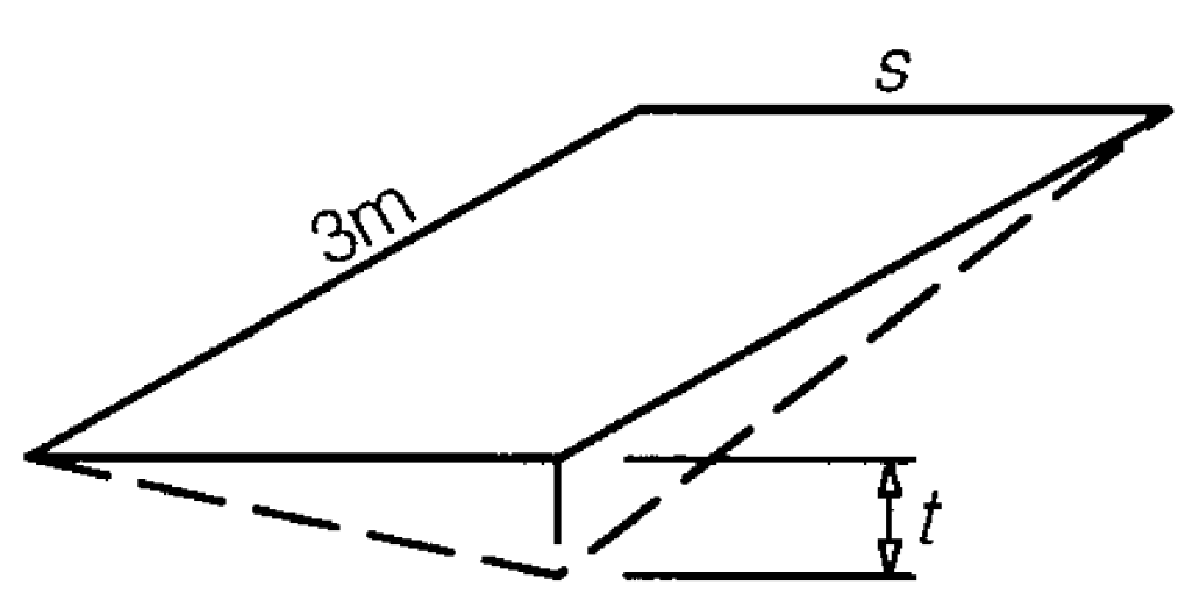
\includegraphics[width=0.8\textwidth]{definitiondecktwist.pdf}
	\caption{Definition of deck twist. Extracted from \cite[Figure A2.1]{1990a2}}
	\label{fig:difinitiondecktwist}
\end{figure}

\paragraph{Vertical deformations}
For all the structures configurations, loaded with the classified characteristic vertical LM 71, or with the models SW/0 and SW/2 if required, the maximum  total vertical deflection measured along any track due to railway traffic actions should not exceed $L/600$. The angular rotations at the end of decks, represented in Figure.\ref{fig:difinitionangularrotations} , in the vicinity of expansion devices, switches and crossings, should be verified.

\begin{figure}[h]
	\centering
	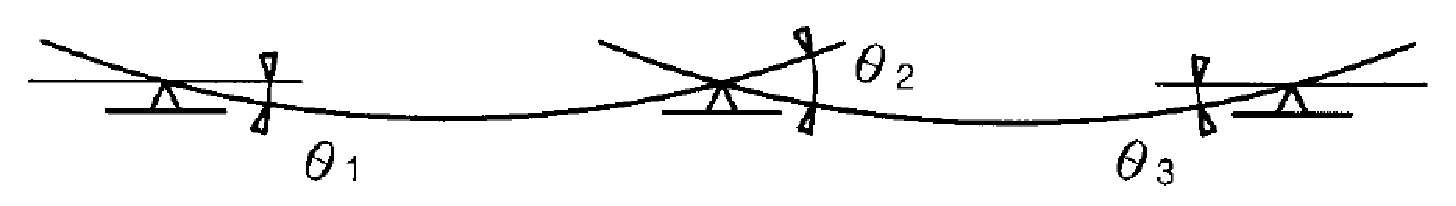
\includegraphics[width=0.8\textwidth]{definitionangularrotations.pdf}
	\caption{Definition of anular rotations at the end of the decks. Extracted from \cite[Figure A2.2]{1990a2}}
	\label{fig:difinitionangularrotations}
\end{figure}

\paragraph{Transverse deformations and vibrations}\label{sec:Transverse-deformations-and-vibrations}
\cite[A2.4.4.2.4]{1990a2}  proposed that transverse deformation and vibration of the deck shall be checked for characteristic combinations of Load Model 71 and SW/0 as appropriate multiplied by the dynamic factor $\phi$ and $\alpha$ (or real train with the relevant dynamic factor if appropriate), wind loads, nosing force, centrifugal forces in accordance with \cite[6]{EC12} and the effect of a transverse temperature differential across the bridge.

The transverse deflection $ \delta_h $ at the top of the deck should be limited to ensure:

\begin{enumerate}
	\item a horizontal angle of rotation of the end of a deck about a vertical axis not greater than the values given in Table.~\ref{tab:maximumhorizontalrotation} , or
	\item the change of radius of the track across a deck is not greater than the values in Table.~\ref{tab:maximumhorizontalrotation} , or
	\item at the end of a deck the differential transverse deflection between the deck and adjacent track formation or between adjacent decks does not exceed the specified value
\end{enumerate}

\begin{table}[h]
	\centering
	\begin{tabularx}{0.8\textwidth}{cXcc}
	\hline
	Speed range V(km/h) & Maximum horizontal rotation(radian) & \multicolumn{2}{c}{Maximum change of radius of curvature}\\
	& & Single deck & Multi-deck bridge\\
	\hline
	$ V\leq 120 $ & $ \alpha_1 $ & $ r_1 $ & $ r_4 $ \\
	$ 120\leq V \leq 200 $ & $\alpha_2 $ & $r_2$ & $ r_5 $ \\
	$V>200$ & $ \alpha_3 $ & $r_3$ & $r_6$\\
	\hline
	\end{tabularx}
	\\
	NOTE 1 The change of the radius of curvature may be determined using:
			$$ r = \frac{L^2}{8 \delta_h}$$
			
	NOTE 2 The transverse deformation includes the deformation of the bridge deck and the substructure(including piers, piles and foundations).
			
	NOTE 3 The values for the set of $\alpha_i$ and $r_i$ may be defined in the National Annex. The recommended values are:
			
	$ \alpha_1 = 0.0035$; $\alpha_2=0.0020$; $\alpha_3=0.0015$;
			
	$ r_1  =1700$; $r_2=6000$; $r_3=14000$;
			
	$ r_4 = 3500$; $r_5 = 9500$; $ r_6 = 17500$
	
	\caption{Maxiumum horizontal rotation and maximum change of radius of curvature}
	\label{tab:maximumhorizontalrotation}
\end{table}

The first natural frequency of lateral vibration of a span should not be less than $f_{h0}$. The value for $f_{h0}$ may be defined in the National Annex. The recommended value is: $f_{h0}=1.2 Hz$

\paragraph{Longitudinal displacements}
For rails on the bridge and on the adjacent abutment, the permissible additional rail stresses due to the combined response of the structure and the track, due to variable actions, should be limited to the following design values:

\begin{enumerate}
	\item Compression: $72KN/mm^2$
	\item Tension: $92KN/mm^2$
\end{enumerate}

\begin{figure}[p]
	\centering
	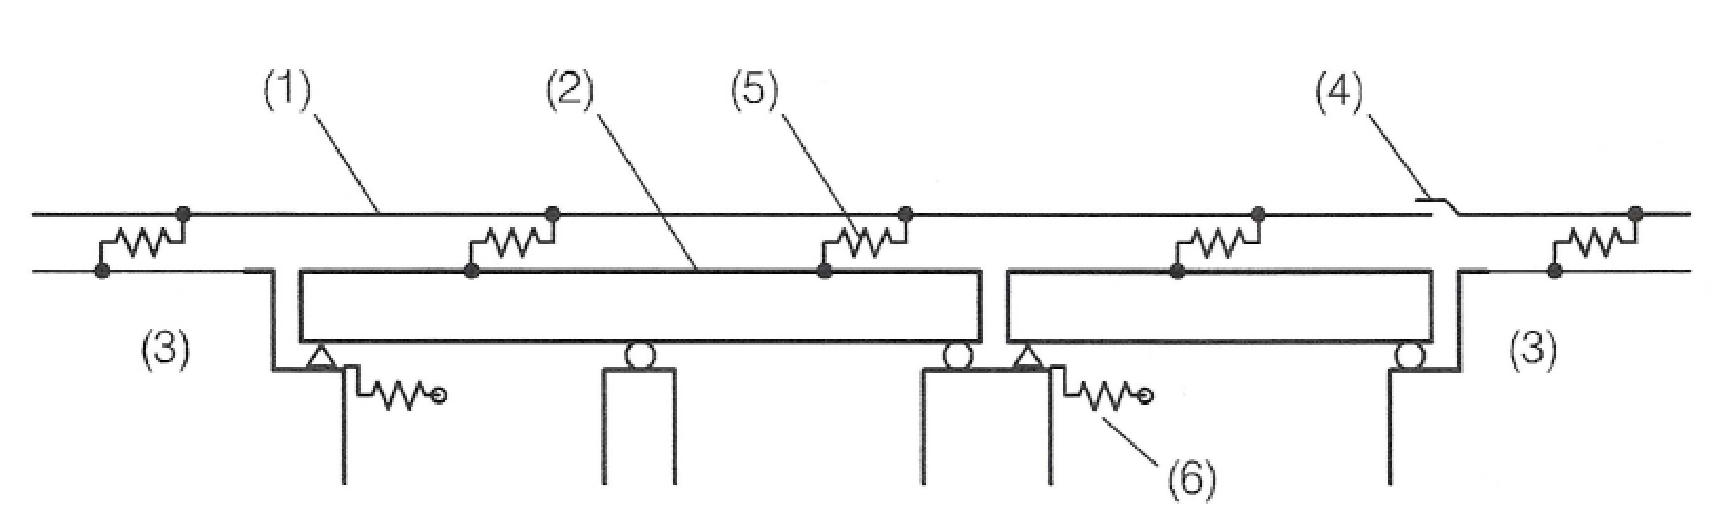
\includegraphics[width=0.8\textwidth]{modeltrackstructure.pdf}
	\caption{Model of a track/structure system. Extracted from \cite[Figure 6.19]{EC12}}
	\label{fig:modeltrackstructure}
\end{figure}

\begin{figure}[p]
	\centering
	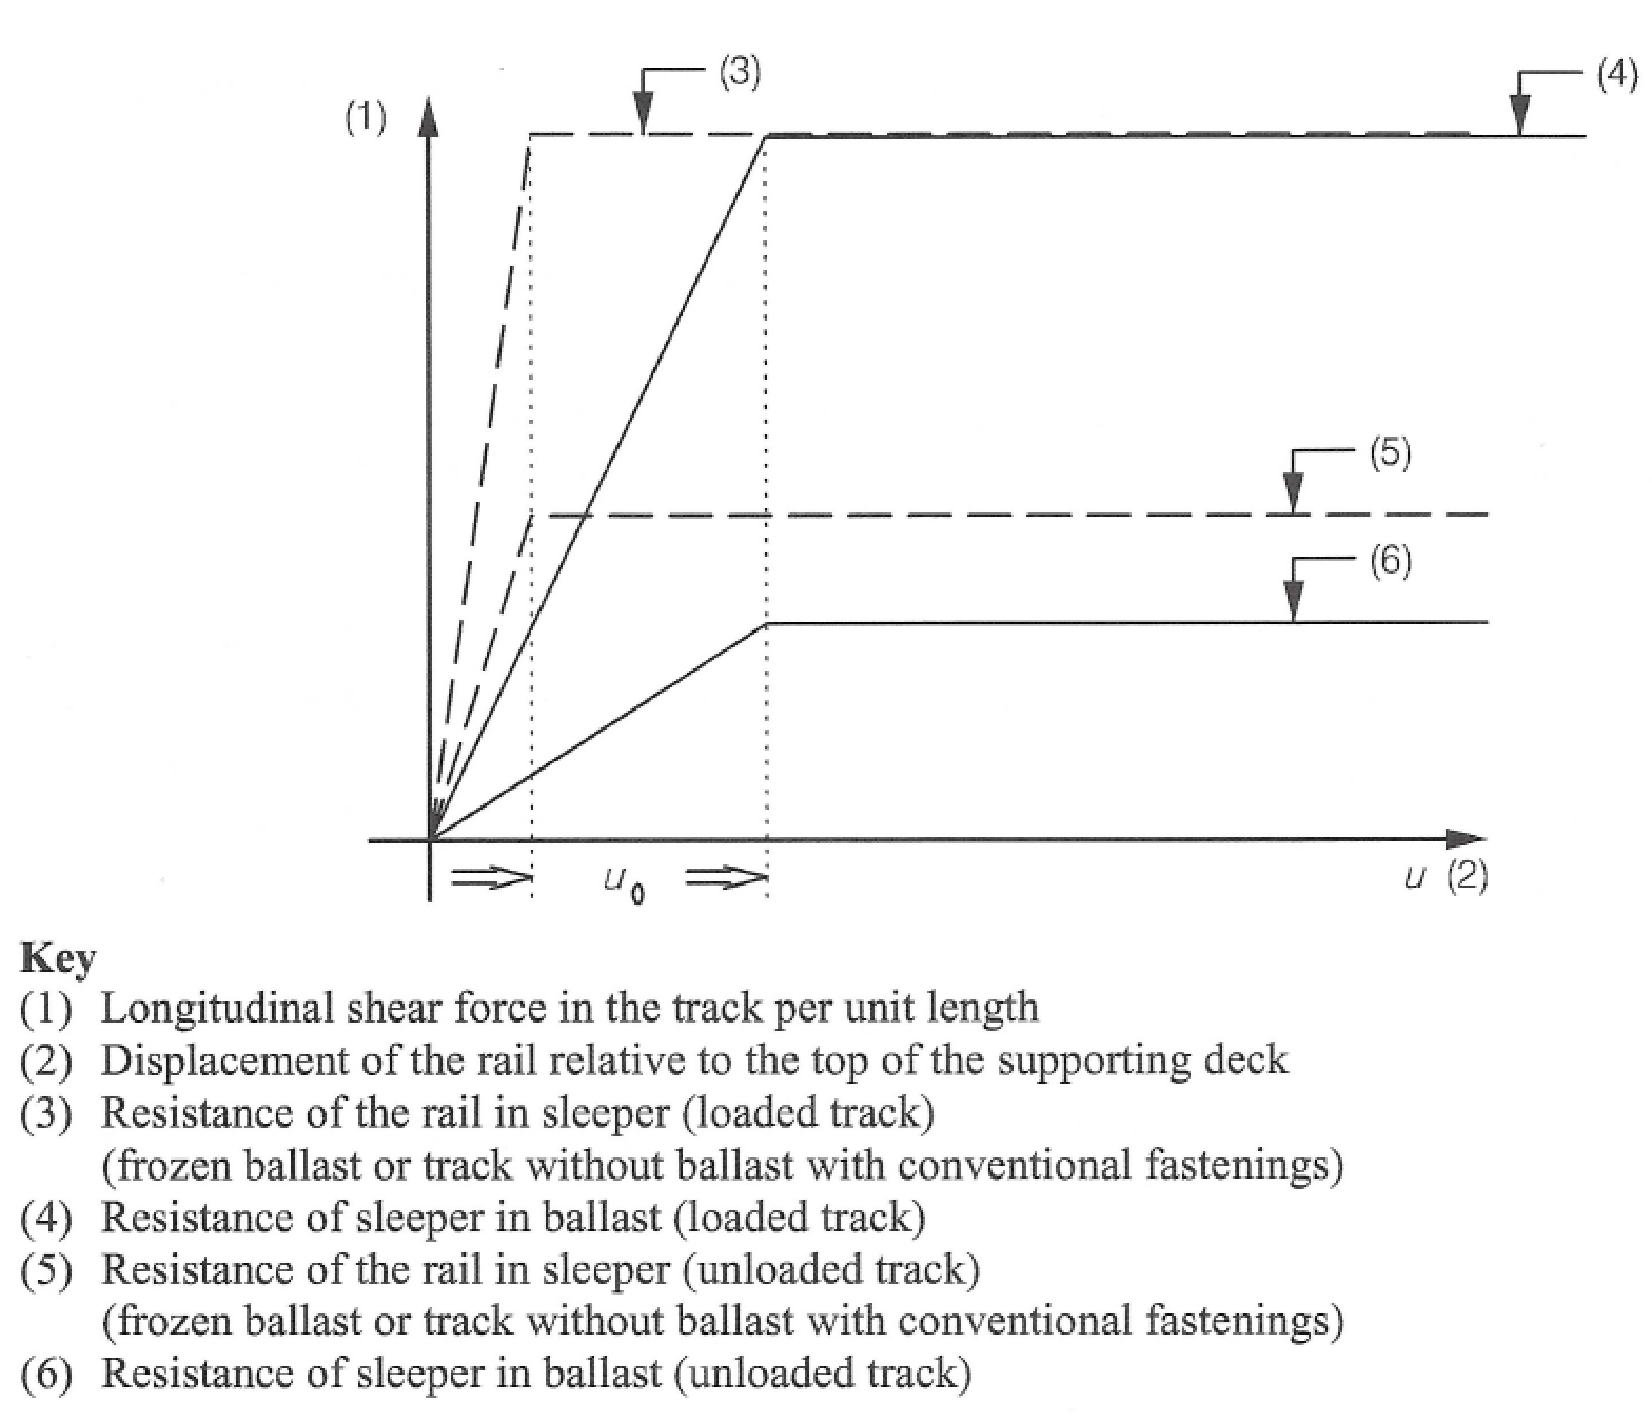
\includegraphics[width=0.8\textwidth]{variationlongitudinalshearforce.pdf}
	\caption{Variation of longitudinal shear force with longitudinal track displacement for one track. Extracted from \cite[Figure 6.20]{EC12}}
	\label{fig:variationlongitudinalshearforce}
\end{figure}

When determining the combined response of track and structure to traction and braking forces, these forces should not be applied on the adjacent embankment unless a complete analysis is carried out considering the approach, passage over and departure from the bridge of rail traffic on the adjacent embankments to evaluate the most adverse load effects.

For the determination of load effects in the combined track/structure system a model based upon Figure\ref{fig:modeltrackstructure} may be used where the longitudinal load/displacement behaviour of the track or rail supports may be represented by the relationship shown in Figure.\ref{fig:variationlongitudinalshearforce}.

Model in Figure\ref{fig:modeltrackstructure} is very important to evaluate the security of the track structure and not the structural security. High track deformations can lead to unfavourable effects for the structure and for vehicles when these are crossing the bridge.

\subsubsection{Serviceability limit states - passenger comfort}

For these type of verifications \cite{1990a2} defines the limiting values for the maximum vertical deflection for passenger comfort, as following:

\begin{enumerate}
	\item Comfort criteria
	\item Deflection criteria for checking passenger comfort
	\item Requirements for a dynamic vehicle/bridge interaction analysis for checking passenger comfort
\end{enumerate}

Passenger comfort depends on the vertical accelerations, $b_v$, inside the coach. These levels of comfort limiting values for the vertical accelerations are presented in Table.\ref{recommendedaccelerationsvalues}

\begin{table}[h]
	\centering
	\begin{tabular}{cc}
		\hline
		Very good & $1.0m/s^2$ \\
		Good & $1.3 m/s^2$ \\
		Acceptable & $2.0m/s^2$\\
		\hline
	\end{tabular}
	\caption{Recommended accelerations values to ensure the respective levels of comfort. Extracted from \cite[Table A 2.9]{1990a2}.}
	\label{recommendedaccelerationsvalues}
\end{table}

\begin{figure}[h]
	\centering
	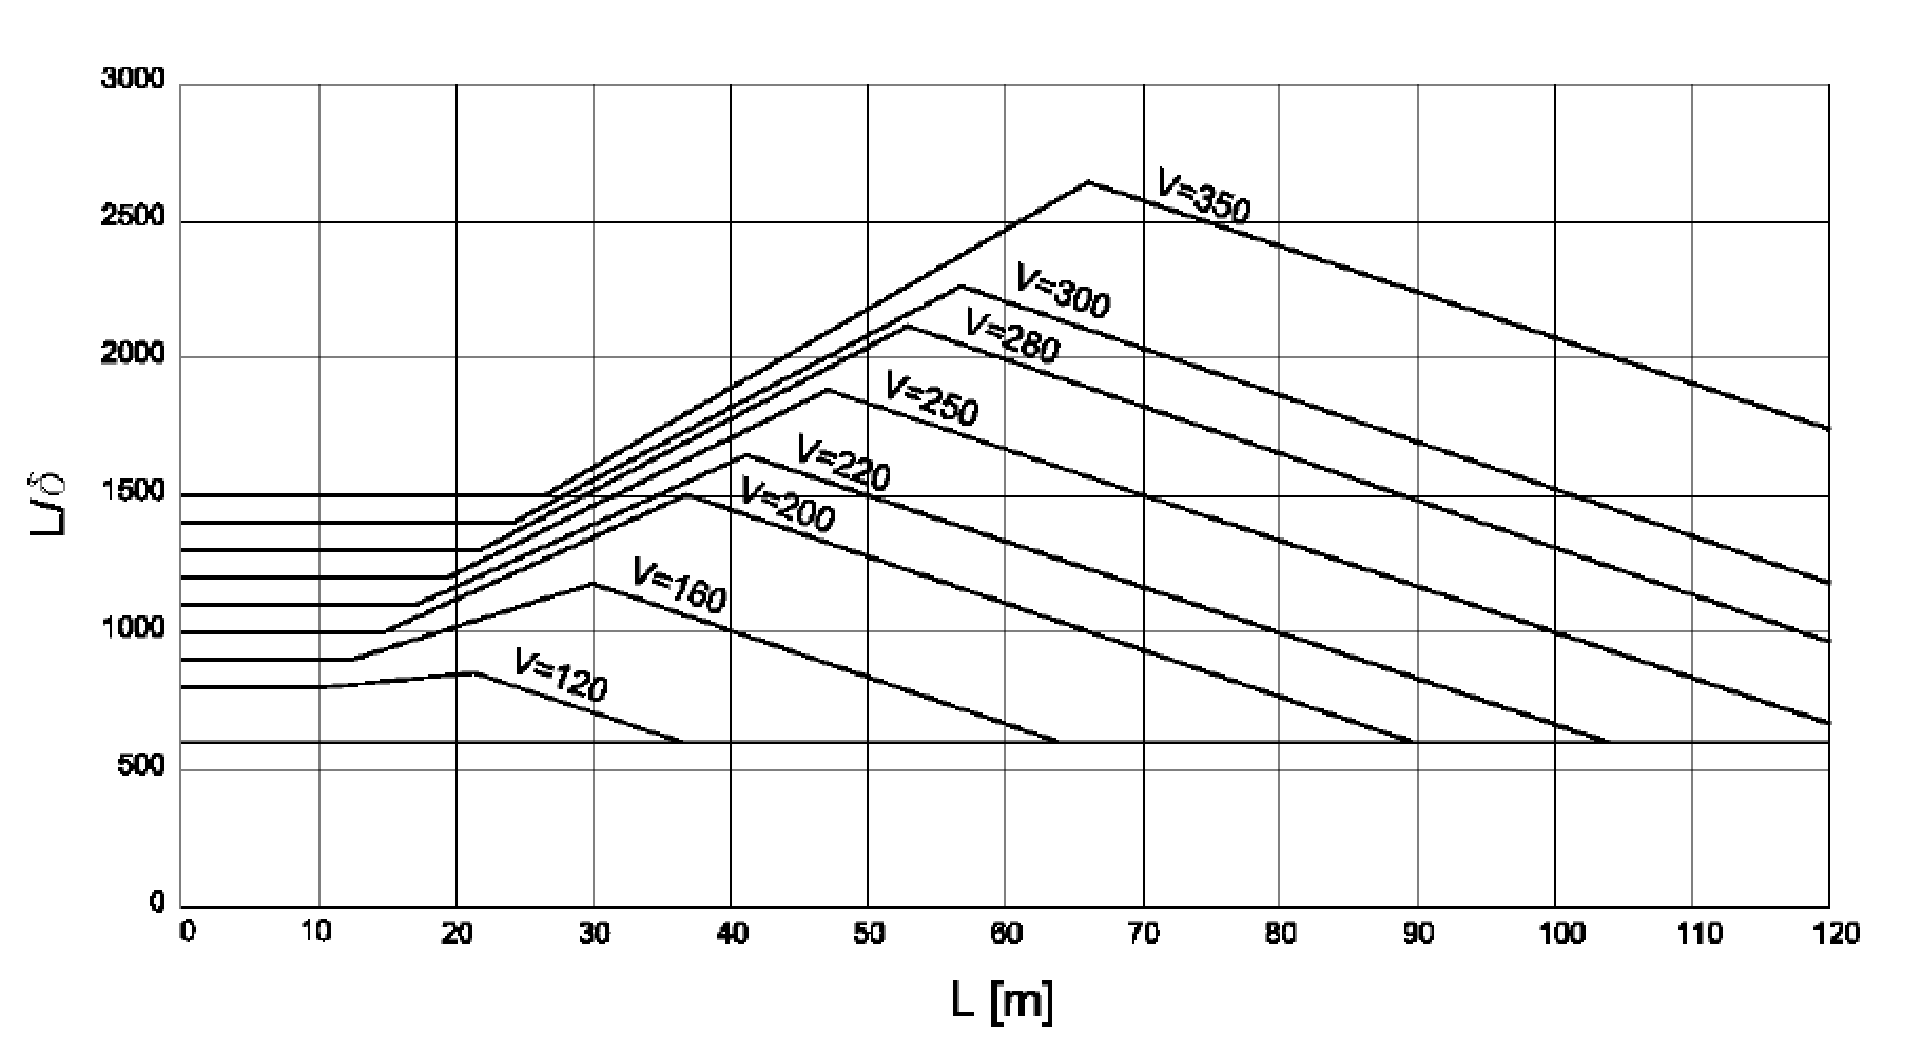
\includegraphics[width=0.8\textwidth]{recommendedlevelofcomfort.pdf}
	\caption{Maximum permissible vertical deflection $\delta$ for railway bridges with 3 or more successive simply supported spans corresponding to a permissible vertical acceleration of $b_v=1m/s^2$ in a coach for speed $V$[km/h]. Extracted from \cite[Figure A2.3]{1990a2}}
	\label{fig:recommendedlevelofcomfort}
\end{figure}

In order to limit vertical vehicle acceleration, being the limits defined in Table\ref{recommendedaccelerationsvalues},vertical displacements should be less than the maximum permissible vertical deflection, $\delta$, obtained from Figure\ref{fig:recommendedlevelofcomfort}. These values are expressed in function of the span length $L$[m], and train speed $V$[km/h], which is valid only for railway bridges with three or more successive simply supported spans. Alternatively these accelerations can be determined considering the vehicle-structure interaction dynamic analysis.

Additionally, the limiting values of $L/\delta$, defined in Figure\ref{fig:recommendedlevelofcomfort} are given for $b_v=1.0m/s^2$.

Vertical deflections should be determined with the LM 71 model multiplied by the factor $\phi$ and adopting $\alpha=1$, being only one track loaded for the case of bridges with two or more tracks.

\subsection{Principal supplementary checks}
\subsubsection{Verification of maximum peak deck acceleration along each track}
\subsubsection{Verification of whether the calculated load effects from high-speed rail traffic, including HSLM on high-speed interoperable routes, are greater than those of normal rail traffic loading(LM71''+''SW/0)}
\subsubsection{Additional verification for fatigue where dynamic analysis is required}
\subsubsection{Verification of limiting values for the maximum vertical deflection for passenger comfort}

\subsection{Diagram of general procedures}
By summarizing Eurocode several steps of calculation are extracted as following, arranged in chronological order.

\begin{enumerate}
	\item  Follow the conceptual check to avoid unsafe designs
	\item  Follow the logic diagram in Figure~\ref{fig:logicdiagram} to check whether dynamic analyses are required 
	\item  Find the appropriate train models, including 
	\begin{enumerate}
		\item-Hypotheses relating to rolling stock
		\item-Rolling stock for interoperability
		\item-Load models HSLM
		\item-Load distribution
		\item-Load combinations and partial factors
		\item-Train speeds to be considered
	\end{enumerate}
	\item Perform the static analyses
	\item  Examine bridge parameters, including
		\begin{enumerate}
			\item-Structural damping
			\item-Mass of the bridge
			\item-Stiffness of the bridge
		\end{enumerate}
	\item Perform the dynamic analyses
	\item  Principal supplementary design checks, including
	\begin{enumerate}
		\item-Verification of maximum peak deck acceleration along each track
		\item-Verification of whether the calculated load effects from high-speed rail traffic, including HSLM on high-speed interoperable routes, are greater than those of normal rail traffic loading(LM71''+''SW/0)
		\item-Additional verification for fatigue where dynamic analysis is required
		\item-Verification of limiting values for the maximum vertical deflection for passenger comfort
	\end{enumerate}
	\item The results of the dynamic analysis shall be compared with the results of the static
analysis multiplied by the dynamic factor $\varPhi$ in 6.4.5 The most unfavourable values of the load effects shall be used. 
\end{enumerate}

\section{Dynamic analysing methods}\label{sec:dynamic-analysing-methods}
There are several dynamic analysing methods developed in Europe over time since Eurocodes don't specify what method to be used during dynamic analysing. These methods differ from each other in the level of calculation complexity. For example, Dynamic train signature method is a good solution for simple structures with well-known train types since it cost less time and effort. On the other hand, Train-vehicle method is an inevitable process for some complicated bridge structures thanks to its wide applicability. However, generally, Train-vehicle method is much more time and money consuming. In following paragraphs, some state-of-art dynamic analysing methods will be reviewed.


\subsection{Method based on impact factor}

\subsection{Method based on dynamic train signature}
As mentioned in \cite[A.4.3]{uic}, the dynamic signature of a train is obtained by breaking down the load diagram of a train in Fourier series and by extrapolating it to the natural modes. It represents the dynamic excitation features of the train and is independent of the characteristics of the structure. The signature depends on axle spacing and loads only. However, newly developed Train dynamic signature method like LIR method takes structure characteristics into account, giving more applicable solutions for specific bridge projects.

Train dynamic signature is a useful method of producing quick analyses on resonance characteristics of the vehicle-bridge systems. The method is especially effective for simple bridge structures.

\subsubsection{DER method}

DER = Decomposition of the Resonance Excitation

The development used in DER method begins from the analysis of the frequency of excitation produced by a train of moving loads. This method is based in the following assumptions:

\begin{enumerate} [-]
	\item Applicable only on statistically determined bridges
	\item For the analysis of statistically determined bridges, is considered that the dynamic response is significantly represented by the first mode of vibration
\end{enumerate}

The development of the method is summarised as follows:

\begin{enumerate}
	\item Reduce the response of a statistically determinate beam to a single degree of freeedom system
	\item Decomposition of the dynamic response of the bridge, in Fourier series;
	\item Consideration of the term which corresponds to the condition of resonance frequencies.
\end{enumerate}

The maximum accelerations at the midspan of the beam for a certain speed, is given as follows:

\begin{equation}
	\ddot{y}(t)\leq C_t\cdot A(L/\lambda)\cdot G(\lambda)
\end{equation}

where the first factor is a constant that depends from bridge characteristics:

\begin{equation}
	C_t=\dfrac{8\pi f_0^2}{K}=\dfrac{4}{\rho\pi L}  
\end{equation}

The second factor is a function called dynamic influence line:

\begin{equation}
	A(L/\lambda )= \bigg\vert\dfrac{\cos (\pi L/\lambda)}{(2L/\lambda)^2-1} \bigg\vert
\end{equation}

and the third factor represents the train dynamic signature, defined as follows:

\begin{equation}
	G(\lambda)=\sqrt{[\sum_{k=1}^N F_k\cos(\dfrac{2\pi x_k}{\lambda})]^2+[\sum_{k=1}^N F_k \sin(\dfrac{2\pi x_k}{\lambda})]^2}\cdot (1-e^{-2\pi \xi \dfrac{x_N}{\lambda}})\cdot \dfrac{L}{\xi x_N}
\end{equation}

\subsubsection{LIR method}
LIR method is based on residual influence line. It is applicable only on statistically determined bridges, too. The solution of the displacements and accelerations in the midspan, of the simply supported beam, is developed by \citeauthor{dominguez2001dinamica}. The solution is given as follows:

\begin{equation}
	\centering
	y_{max}=C_{desp}\cdot A(r) \cdot G(\lambda)
\end{equation}

\begin{equation}
	\ddot{y}_{max}=C_{acel}\cdot A(r) \cdot G(\lambda)
\end{equation}

with,

\begin{equation}
	C_{desp} = \frac{1}{M\omega_0^2},
	C_{acel} = \frac{1}{M}
\end{equation}

The factor $ A(r) $ is the dynamic influence line, give as:

\begin{equation}
	A(r)=\frac{r}{1-r^2}\sqrt{e^{-2\xi \frac{\pi}{r}}+1+2\cos (\frac{\pi}{r})e^{-2\xi \frac{\pi}{r}}}
\end{equation}

with $ r=\lambda/2L $.

$G(\lambda)$ is named train dynamic signature, depending from train characteristics and from the damping coefficient of the structure, give as follows:

\begin{equation}
\end{equation}

To make $G(\lambda)$ representative for the maximum response, maximum value of $G(\lambda)$ for each different subtrain is considered the value of $G(\lambda)$

\begin{equation}
	G(\lambda) = \max_{i=1}^{N} \sqrt{[\sum_{x_1}^{x_i}F_i\cos (2\pi \delta_i) e^{-2\pi \xi \delta_i}]^2+[\sum_{x_1}^{x_i}F_i \sin (2\pi \delta_i) e^{-2\pi \xi \delta_i}]^2}
\end{equation}

\begin{figure}[h]
	\centering
	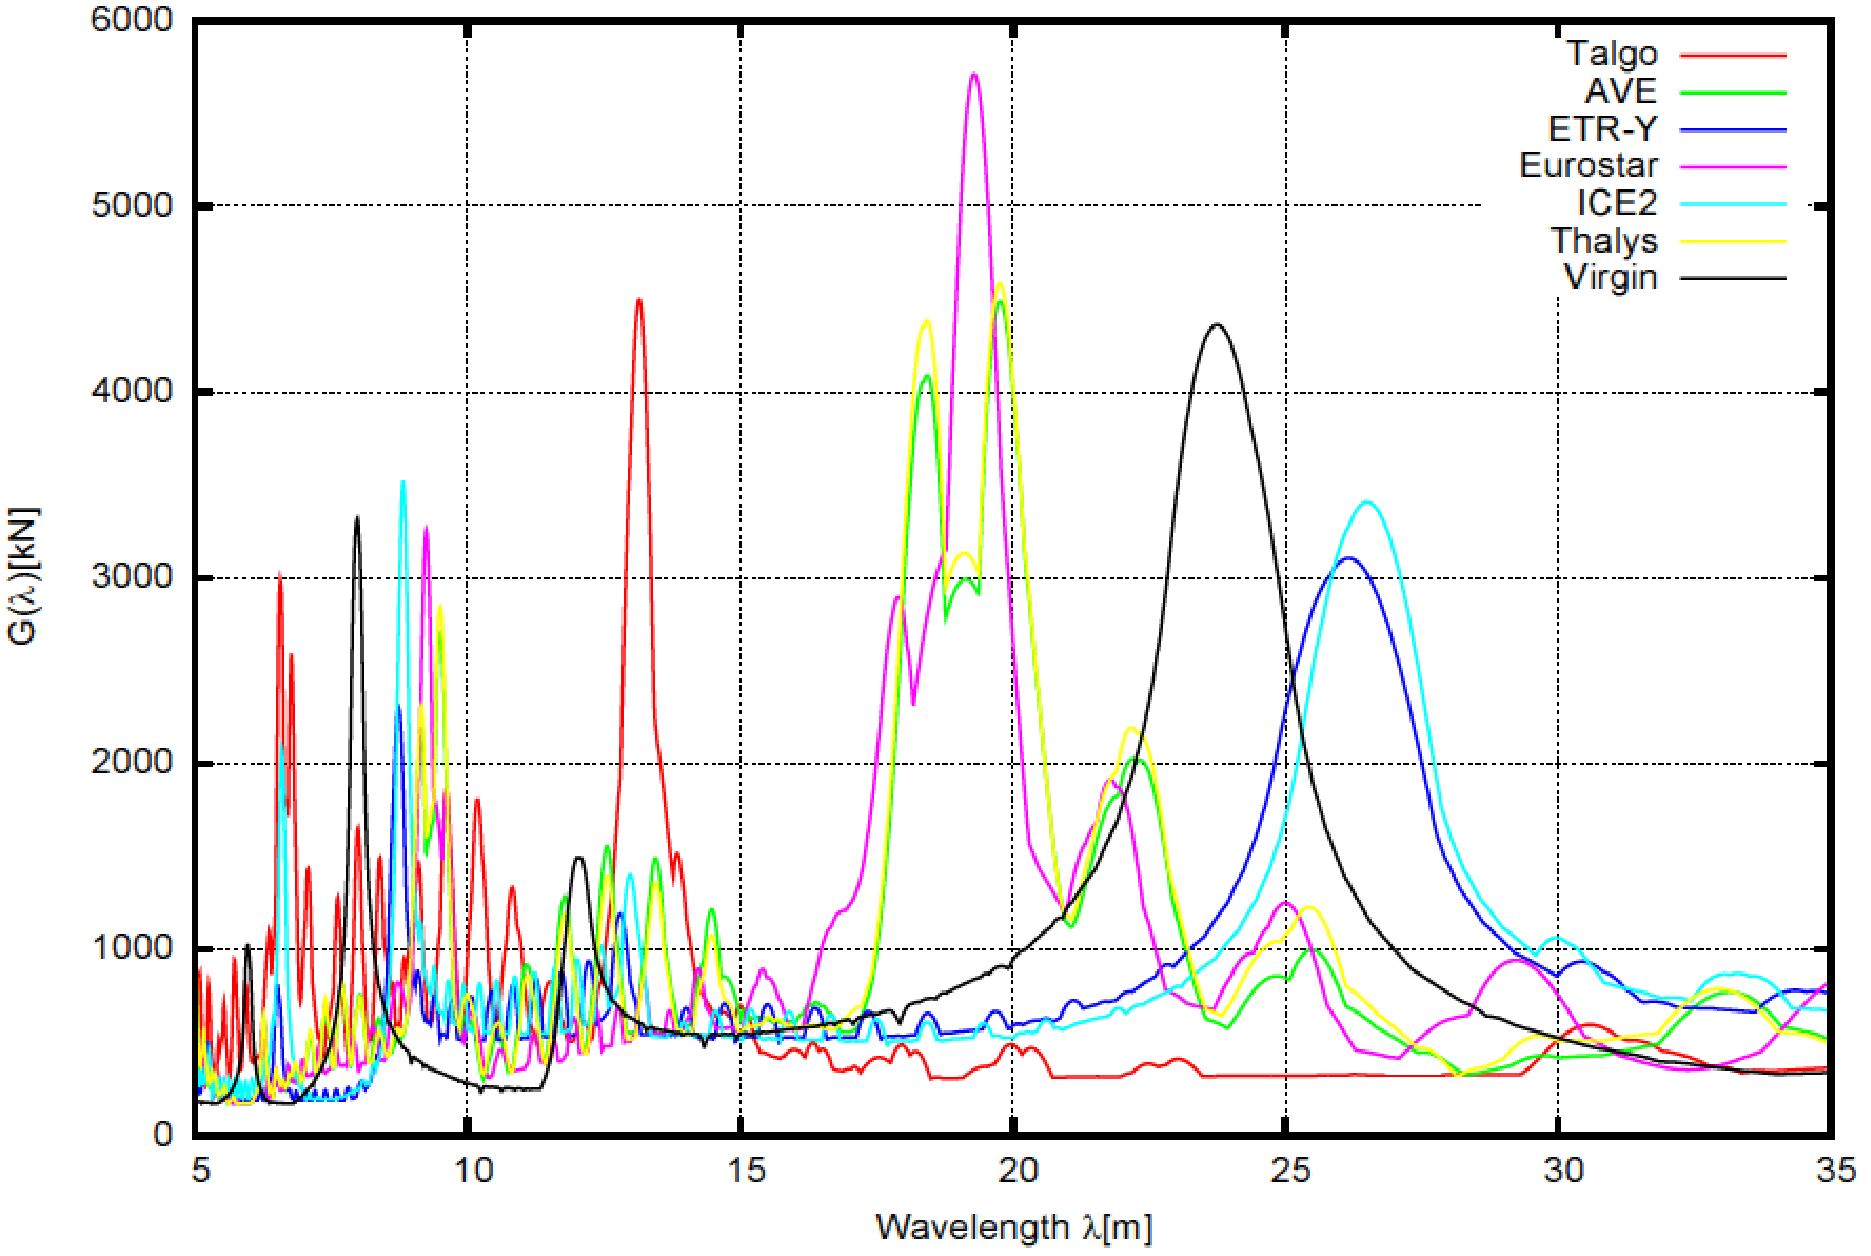
\includegraphics[width=0.6\textwidth]{trainsig.pdf}
	\caption{Train dynamic signatures for the seven real trains, considering a damping value of $\xi = 0.00$. Extracted from \cite[Figure 2.20]{da2007dynamic}}
	\label{trainsig}
\end{figure}

\subsection{Methods based on finite element models}
Finite element methods are the most applicable methods available. The methods are based on direct time integration.

\subsubsection{Direct time integration methods}
General equation of motion for a SDOF system can be given in following form:

\begin{equation}
	\boldsymbol{M\ddot{d}}+\boldsymbol{C\dot{d}}+\boldsymbol{Kd}=\boldsymbol{f}(t)
\end{equation}

where $\boldsymbol{M}$ is the mass matrix, $ \boldsymbol{c} $ is the damping matrix, $ \boldsymbol{K} $ is the stiffness matrix, $ \boldsymbol{f}(t) $ is the vector of external loads and $ \boldsymbol{d} $ the unknown vector of nodal displacements. 

Direct time integration method is the principle of finite element models. Due to the expected huge amount of calculation, computers are used to process time integration calculations. Thanks to the reliability and efficiency of computers, there are more and more project done with the help of computer FEM software nowadays.

\subsubsection{Modelling a train of moving loads}
The method of modelling spatial moving loads in FEM software is applying load histories in each convenient node. At a certain time-step, a load F, whose magnitude depending linearly on the distance from the axle to the node, is assigned to each node if the load axis is above an element that contains the node. The procedure is outlined in Figure.\ref{fig:movingloads}.

\begin{figure}[h]
	\centering
	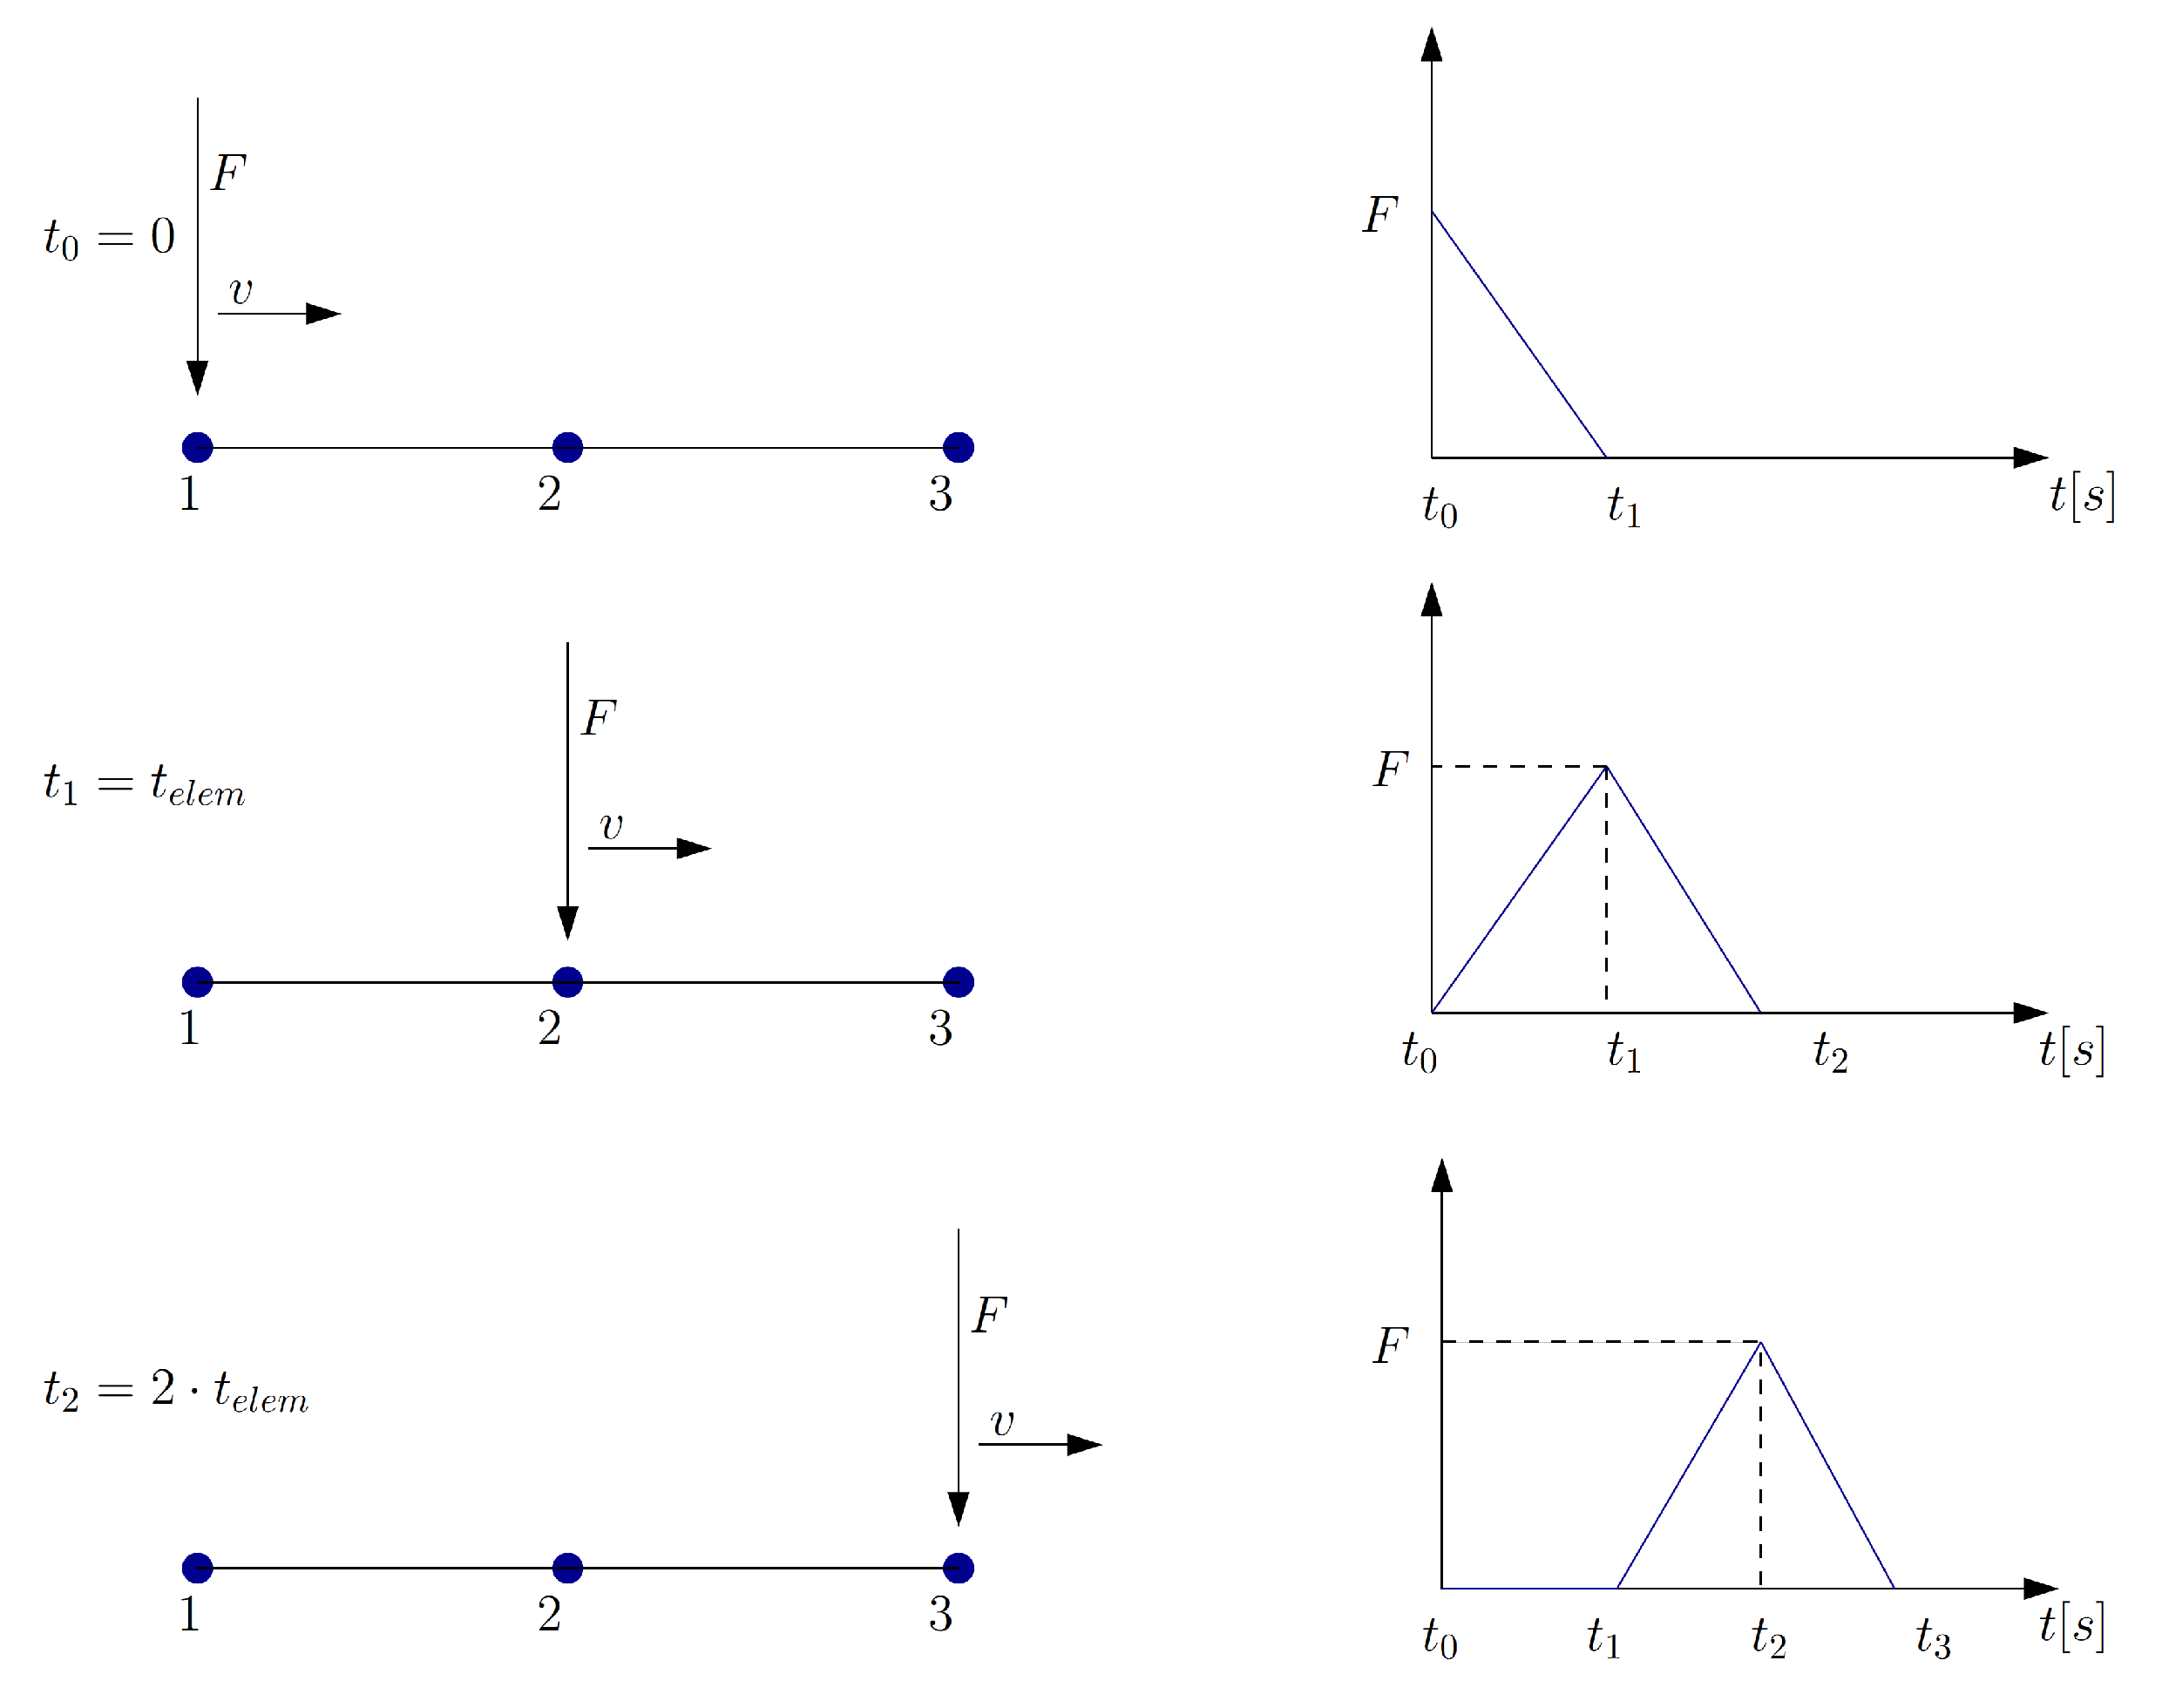
\includegraphics[width=0.8\textwidth]{movingloads.pdf}
	\caption{Nodal force time history definition for a single moving load $F$, with speed $v$. Extracted from \cite[Figure 2.15]{da2007dynamic}}
	\label{fig:movingloads}
\end{figure}

\subsection{Analytical methods based on modal analysis}
Modal analysis is the study of the dynamic properties of structures under vibrational excitation. Applied on railway bridge structures, the analysis can be simple if the bridge is modelled as a simply supported beam.

\subsubsection{Modal analysis of a simply supported beam}
blahblahblahblahblah stuff

\blindtext

Contents to be added

\subsubsection{Modes of vibration}

\blindtext

\subsubsection{Number of modes of vibration to consider in the analysis}

\blindtext


\subsection{Method based on vehicle-Structure interaction dynamic analysis}\label{sec:tds}
Different from point load models, vehicle-structure models takes suspension systems of train vehicles into account, providing associations between train carriage and structure. Impact of suspension system vibration on bridge structure can be neglected when the span of the bridge is comparably small since there's little chance for suspension system and bridge to resonant. As the span of bridges increase, the first vertical/transverse natural frequency of bridge can decrease into the natural frequency range of train suspension system. This means long-span bridges can resonant with train suspension system. To study the effects related to train suspension system, vehicle-structure interaction method is developed. 

A general model for a conventional coach on two bogies are shown in Figure.\ref{fig:vehicle-structure}, including the stiffness and damping $(K_P,c_P)$ of the primary suspension of each axle, the secondary suspension of the bogies $(K_s,c_s)$, the unsprung mass of the wheels $(M_w)$, the bogies $(M_b, J_b)$, and the vehicle body $(M,J)$. Similar models may be developed for articulated or regular trains.

\begin{figure}[h]
	\centering
	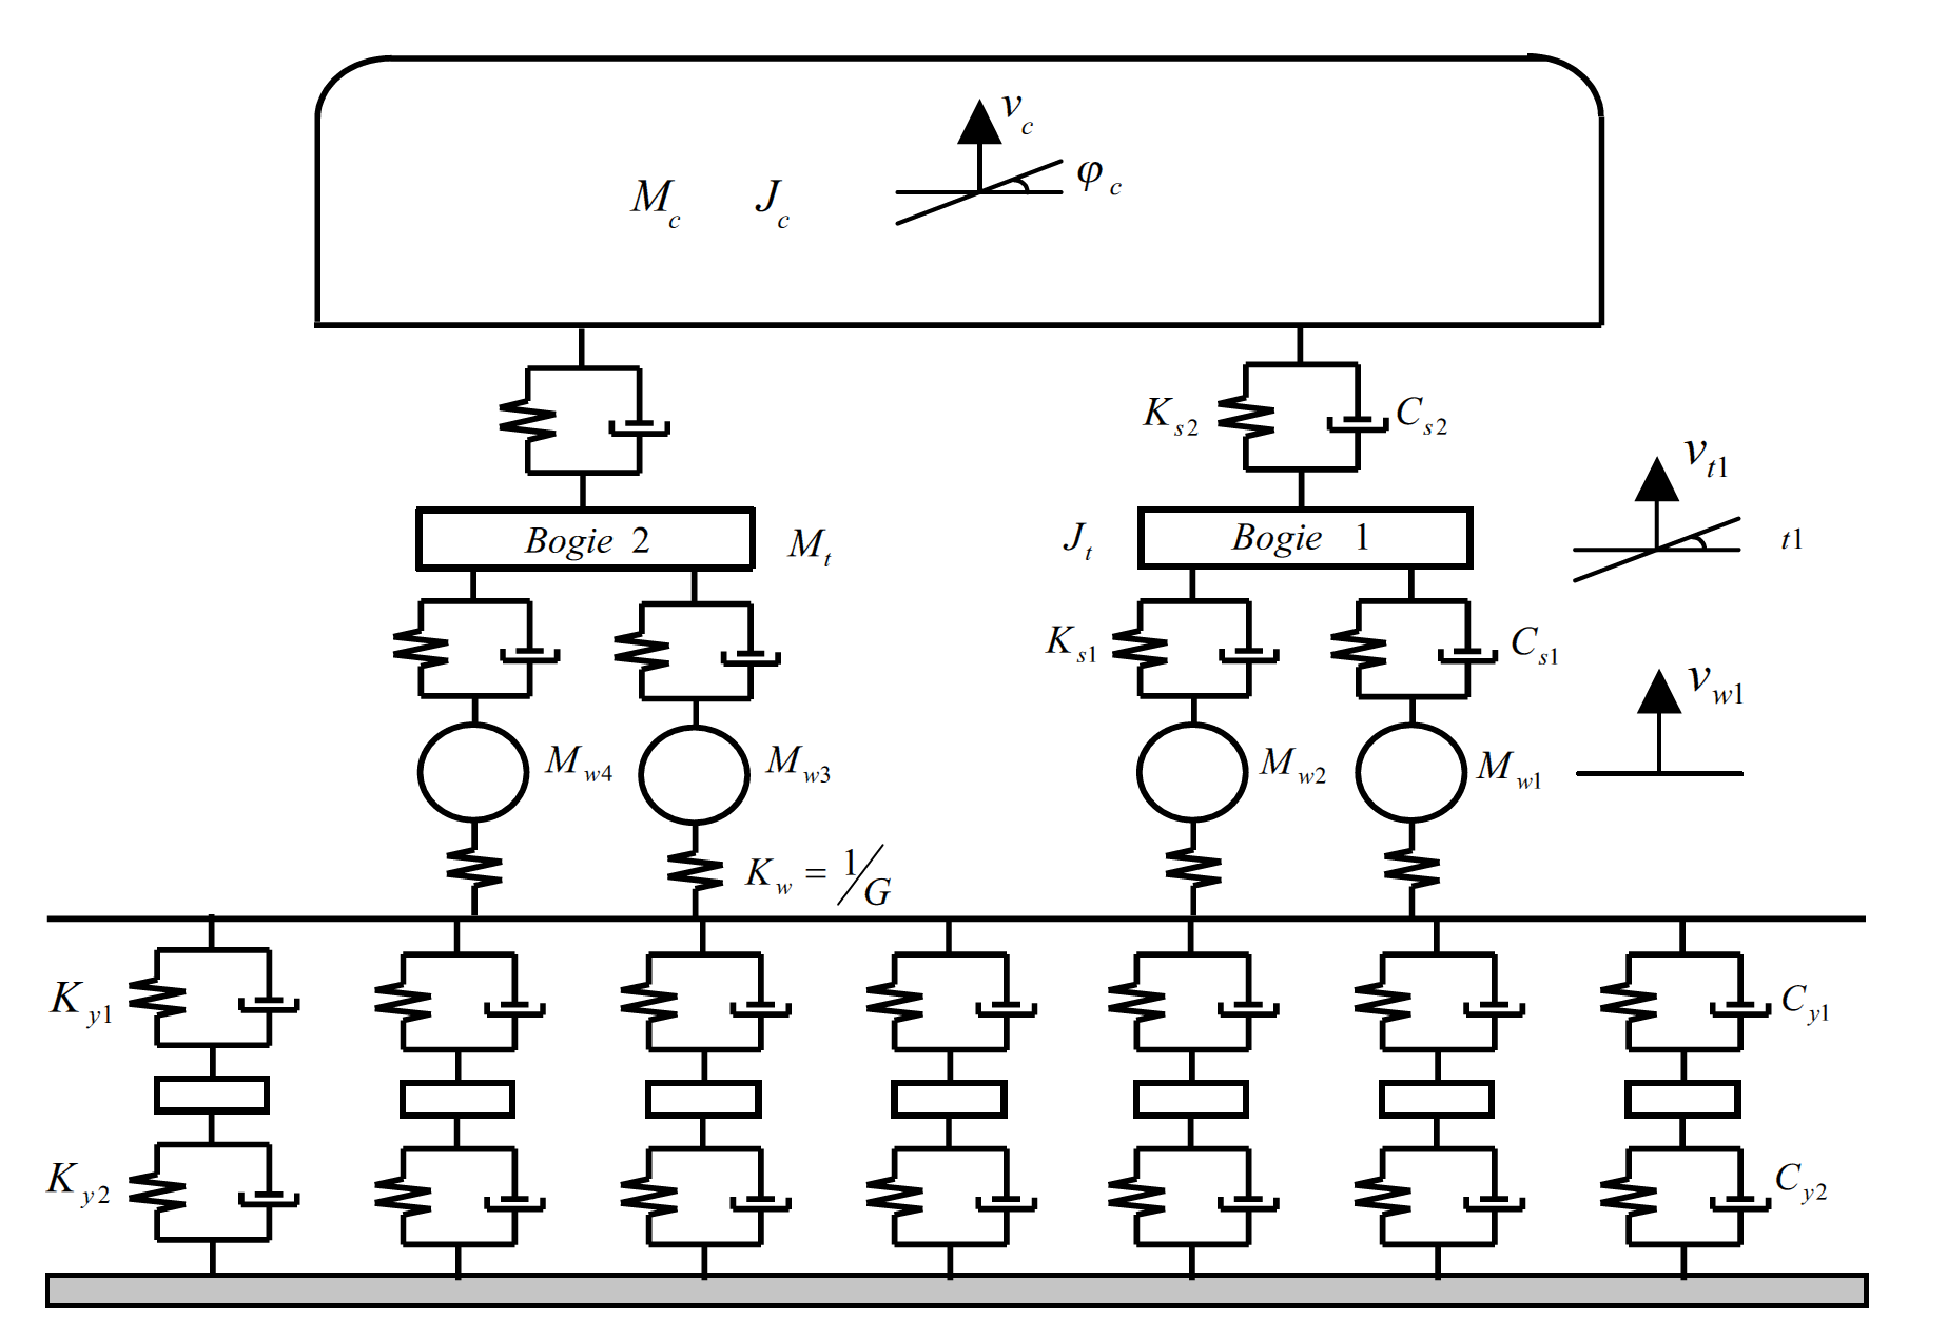
\includegraphics[width=0.8\textwidth]{vehicle-structure.pdf}
	\caption{Model for analysis of vehicle-structure system. Extracted from \cite[Figure 12]{lei2002analyses}}
	\label{fig:vehicle-structure}
\end{figure}

Sometimes more simplified model , represented by one mass, one spring and one damper per bogie can be considered, depending on the purpose of the analysis. See Figure\ref{fig:simplified-vehicle-structure} for example.

\begin{figure}[h]
	\centering
	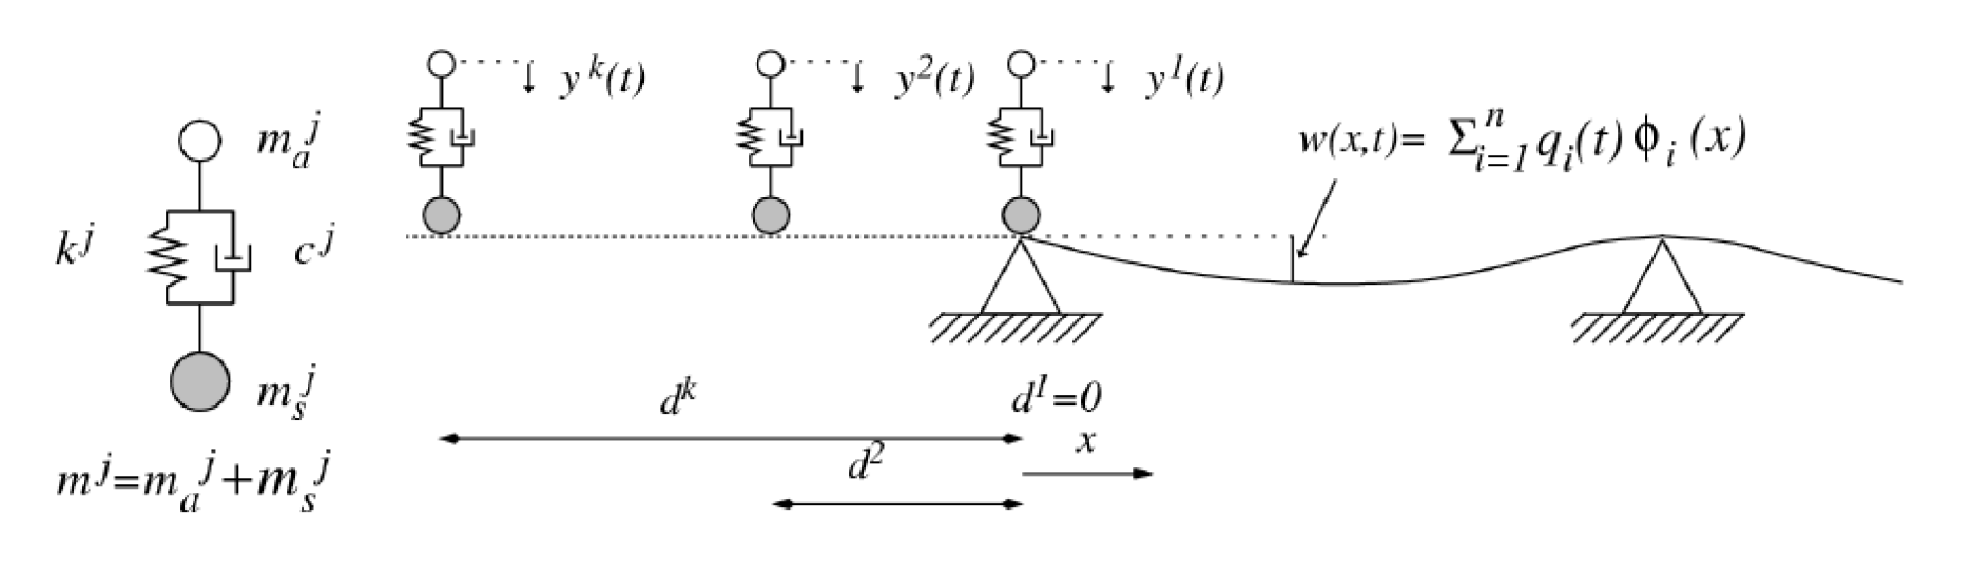
\includegraphics[width=0.8\textwidth]{simplifiedvehiclestructure.pdf}
	\caption{Load train with vehicle-bridge interaction: simplified interaction model and variables definition. Extracted from \cite[Figure15]{lei2002analyses}}
	\label{fig:simplified-vehicle-structure}
\end{figure}
